%chapter 3
\chapter{Boulder-induced YORP Altering Spin Acceleration}
\label{yorp_spin}

\section{Surface Interactions causing YORP}\label{formulation}
%make smooth with last section
%In our simulation and analysis, we find a minimum boulder size and ideal boulder placement for contributing to the YORP effect significantly, which bounds the size of boulder that will be necessary to consider when making YORP predictions. %The paper is organized as follows: in section \ref{background}, we present the background and previous work done regarding modeling asteroid surfaces and YORP, then in section \ref{methods} we outline the methods used to model boulder-induced YORP (BoYORP) including the shapes selected for study,  the simplified thermal model, and the calculation of YORP over a polyhedral shape model with boulders. Next in section \ref{analysis}, we provide the statistical approximations of the boulder factors to be varied in our study. Sections \ref{bennu} and \ref{itokawa} highlights the results found in our Monte Carlo study of many boulder configurations for both asteroid surfaces. We investigate sensitivity of the results to changing biases and size thresholding in section \ref{sens_analysis}, and in section \ref{discussion} discuss these findings and the significance of specific factors of boulder populations. Then the implications of inferring asteroid properties from YORP measurements are discussed in section \ref{implications}. Finally, in section \ref{conclusion}, we summarize the contributions and provide possible pathways for future work. 

The YORP effect was first named by Rubincam, however it had been recognized as a secular component of small body dynamics for many years previous \cite{Rubincam2000}. Today it is observed on many bodies where we are capable of taking high precision measurements of spin rate change over time \cite{Lowry2007}. The general mechanism of YORP is the absorption and re-emission of thermal energy of the surface, dependent on the thermal inertia of the material, incident angle of sunlight, the body's orbit, and the current rotational velocity. The direction of this re-emission is the direction of the YORP force. As this is a force acting on the surface, the force is then translated to a torque about the central spin pole. In Fig.\ref{fig:surface_diagram}, the incident angle of photons is shown by $\alpha$, the angle between the surface normal $\hat{n}$ and the sun direction $\hat{u}$. The force is decomposed into it's normal and transverse components, $d\textbf{F}_{\hat{n}}$ and $d\textbf{F}_t$ respectively. The direction $\hat{s}$ corresponds to the direction of radiation, while $p_{sr}$ and $p_{\hat{u}}$ are the directions of torque due to solar re-radiation and incident solar energy. 
\begin{figure}
    \centering
    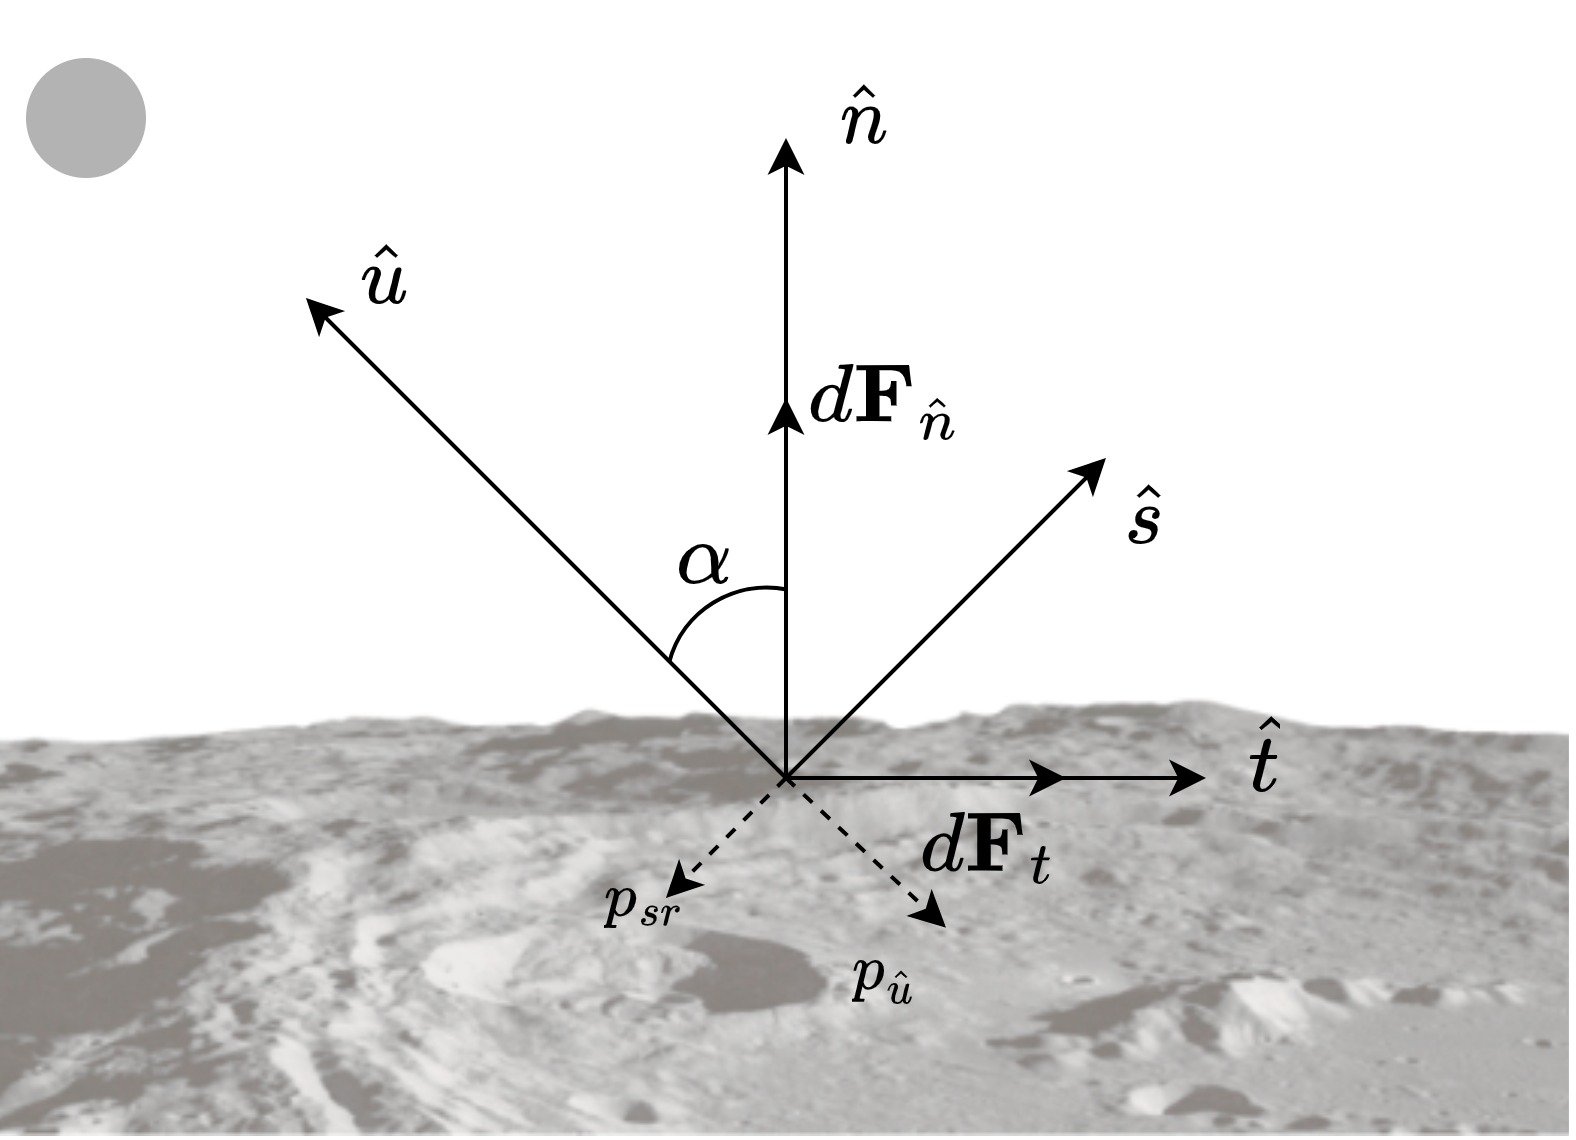
\includegraphics[width=0.45\textwidth]{fig/yorp.jpeg}
    \caption{Diagram of solar radiation, absorption, and YORP re-radiation}
    \label{fig:surface_diagram}
\end{figure}

Statler has shown through simulation that the YORP effect is extremely sensitive to changes in the small-scale topography of a surface, whether Gaussian roughness, craters, or boulders. This work states that at most 50\% of the variance in YORP can be attributed to boulders larger than half the maximum size, which could be just one to five boulders in any given case due to steep power law size distributions \cite{Statler2009}.  Overall, many studies have concluded that YORP is sensitive to small features and that the geometric and thermal properties of these features must be taken into account for a fully representative YORP model \cite{Breiter2009}. 
\\ \indent Different thermophysical models have been proposed to increase accuracy of YORP predictions for surfaces. These models can be one-dimensional or three-dimensional, and instantaneous or time delayed \cite{Rozitis2012}. In this work, we use a one-dimensional instantaneous thermal model which is dependent only on emission directions and assumes diffuse Lambertian re-radiation of photons, and a low surface reflectivity or albedo of 0.05, which represents the dark surfaces seen on rubble-pile bodies such as Bennu \cite{Golish2021}. This is to follow the approximations made by Scheeres for the polyhedral normal YORP model \cite{Scheeres2007}.
\\ \indent Accounting for surface roughness can change predicted YORP torque depending on the magnitude at which it is modeled \cite{Davidsson2014} \cite{Davidsson2015}. One can go down to the microscopic level using the Hapke model for emission directions of regolith as was previously done in an examination of tumbling bodies experiencing YORP \cite{Breiter2011a}.  However, there is a range of roughness at the size regime of the diurnal thermal skin depth (1 cm) and greater that was ignored. This is addressed as thermal-infrared beaming emission modeling done by Rozitis and Green \cite{Rozitis2011}. Roughness was modeled as a combination of craters with varying depths and opening angles, as well as low- and high-resolution Gaussian random height models to represent surface variability at the range of 1 cm to several meters. Results from this modeling show that when directional thermal-infrared beaming is considered for a surface, the YORP torque can be dampened by up to half of its original magnitude for a zero-obliquity rotating body. This model also assumes similar surface geometry as the original smooth facet model, and is therefore not equivalent to modeling boulder features which include new normal directions which perturb the original surface geometry drastically. Modeling boulders, craters, and regolith roughness in tandem correlates a more accurate model for YORP and informs the bounds of variability with higher precision and confidence.  Other dynamical models address the nature of tumbling bodies, which is a possible end-state induced by long-term influence of YORP re-emission \cite{Cicalo2010} \cite{Breiter2015}.  In order to investigate the sensitivity of YORP to boulder parameters, we will continue with a uniform principal-axis rotator that is not near a dynamical end-state of spinning up to disaggregation or spinning down to a dissipative low-energy tumbling state. 

\section{Fourier YORP Coefficient Modeling}
We apply the YORP modeling techniques derived by Scheeres in the polyhedral YORP model. This is an analytical approach to solving for rotational dynamics under YORP perturbation and provides a solution based on discretized shape geometry. The assumptions required for this model are that the body is uniformly rotating on a primary axis, thermal inertia can be parameterized as a constant lag, $T_{lag}$, orbital elements are evolving secularly, and shadowing is considered as an occultation calculation between all facets. For a bulk shape, the force and torque can be decomposed into Fourier coefficients based on the dual periodicity of the asteroid day and year. These coefficients are then used as an approximation for discussing the explicit force and moment, which are related linearly to first-order coefficients through orbital and geometric properties. 


\begin{equation} \label{eq:1}
    \textbf{F} = P(R) \Big[ \textbf{A}_0 + \sum_{n=1}^{\infty} [ \textbf{A}_n \cos(n\lambda) + \textbf{B}_n \sin(n\lambda) ]\Big]
\end{equation}
\begin{equation} \label{eq:2}
    \textbf{M} = P(R) \Big[ \textbf{C}_0 + \sum_{n=1}^{\infty} [ \textbf{C}_n \cos(n\lambda) + \textbf{D}_n \sin(n\lambda) ]\Big]
\end{equation}

Reproduced in Eq.\ref{eq:1} and Eq.\ref{eq:2} is the derived force and moment expressions as Fourier decompositions into coefficients of $n$ order. These relate as $M_i = r_i \times F_i$ and their same-order coefficients (e.g. $C_0$ and $A_0$, etc.) relate similarly. 

\begin{equation}\label{eq:3}
    \mathbf{C}_n = \sum_{i=1}^{N} \mathbf{r}_i \times \mathbf{A}_{n,i}
\end{equation}
Equation \ref{eq:3} is the relationship between the moment coefficients and the force coefficients as they are evaluated over each facet and then summed. As we discuss the YORP coefficient $C_{0}$ in later sections, note that it contains the moment relationship that considers the facet position $r_i$.
This parameterization into coefficients allows the calculation of bulk force using discretized geometric orientation factors and simplified thermal constants. The variable $P(R)$ is the solar pressure as a function of distance of the body from the sun, $R$. The iterative variable $n$ represents the unbounded order of Fourier decomposition, and $\lambda$ is local solar longitude, which is later used in the illumination function to integrate over solar rise and set angles ($\lambda_r, \lambda_s$) for specific facets. 
\\ \indent 
For approximating torque due to features, we focus on the normalized zeroth-order z-component of the moment coefficient, or $\bar{\textbf{C}}_{0,z}$, which can be a function of $\epsilon$, the spin pole obliquity of the asteroid. This value directly correlates to spin evolution due to YORP as shown in Eq.\ref{eq:4}. 
\begin{equation}\label{eq:4}
    \dot{\omega} = \frac{G_1}{I_z a^2 \sqrt{1-e^2}} \bar{\textbf{C}}_{0,z}(\epsilon)
\end{equation}
The angular acceleration is calculated from orbit parameters (semi-major axis $a$, eccentricity $e$, and obliquity $\epsilon$), mass distribution ($I_z$), and incident solar flux ($G_1$) scaled by the orbit-averaged spin coefficient. The YORP spin coefficient is derived from a global summation of re-emitted thermal radiation over the surface area while within illumination bounds. In future work, the orbit-averaged first-order moment coefficients in the x- and y-directions ($\bar{C}_{1,x}, \bar{C}_{1,y}, \bar{D}_{1,x},$ and $\bar{D}_{1,y}$) may be addressed as they pertain to the change in obliquity over time which leads to coupled changes in the spin. This work is focused on the spin-evolution and will only briefly mention obliquity torques due to boulders here. 
 For further explanation of the procedures necessary to evaluate these coefficients, see Scheeres 2007, Sections 3.2 and Appendix A \cite{Scheeres2007}. The next section will focus on the model design developed to calculate boulder-induced YORP torque through this polyhedral approach. 

\section{Boulder Simulation Design} \label{methods} %section 3
\begin{figure*}[t!]
    \begin{subfigure}{0.45\textwidth}
        \centering
        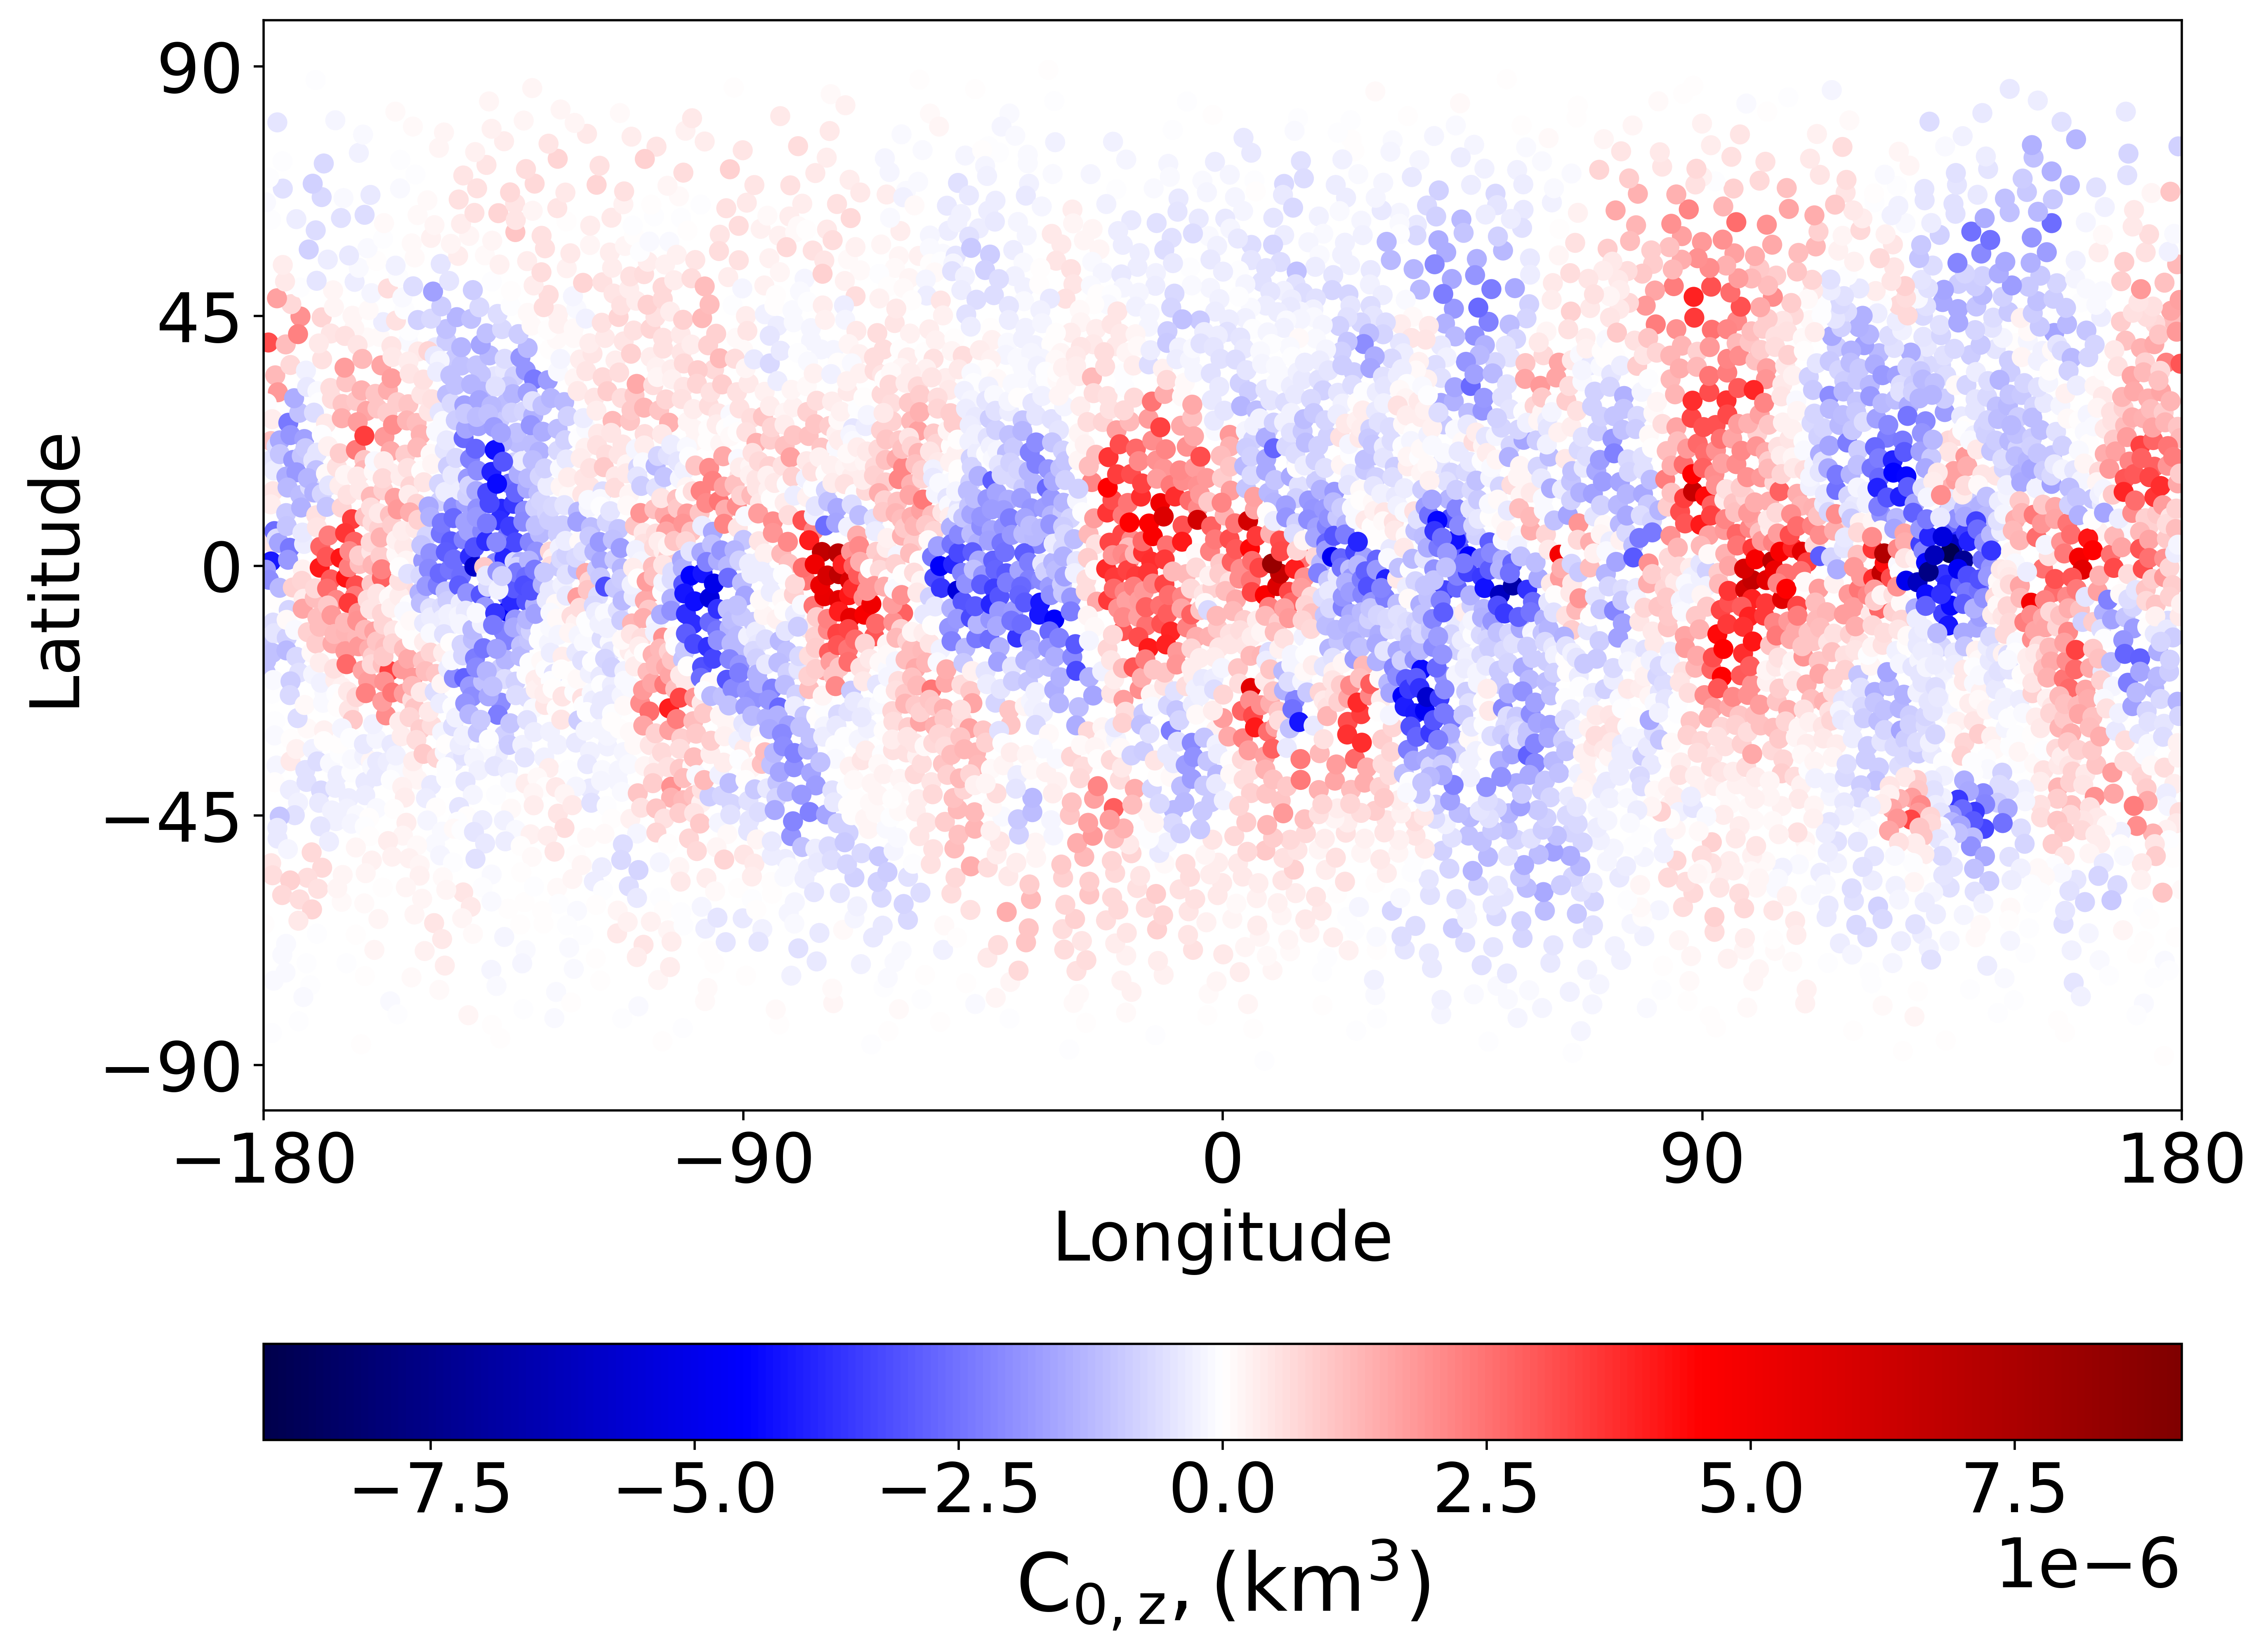
\includegraphics[width=\textwidth]{fig/bennu_base_facet_yorp.png}
        \caption{Bennu Surface YORP per facet}
    \end{subfigure}
    \hfill
    \begin{subfigure}{0.45\textwidth}
        \centering
        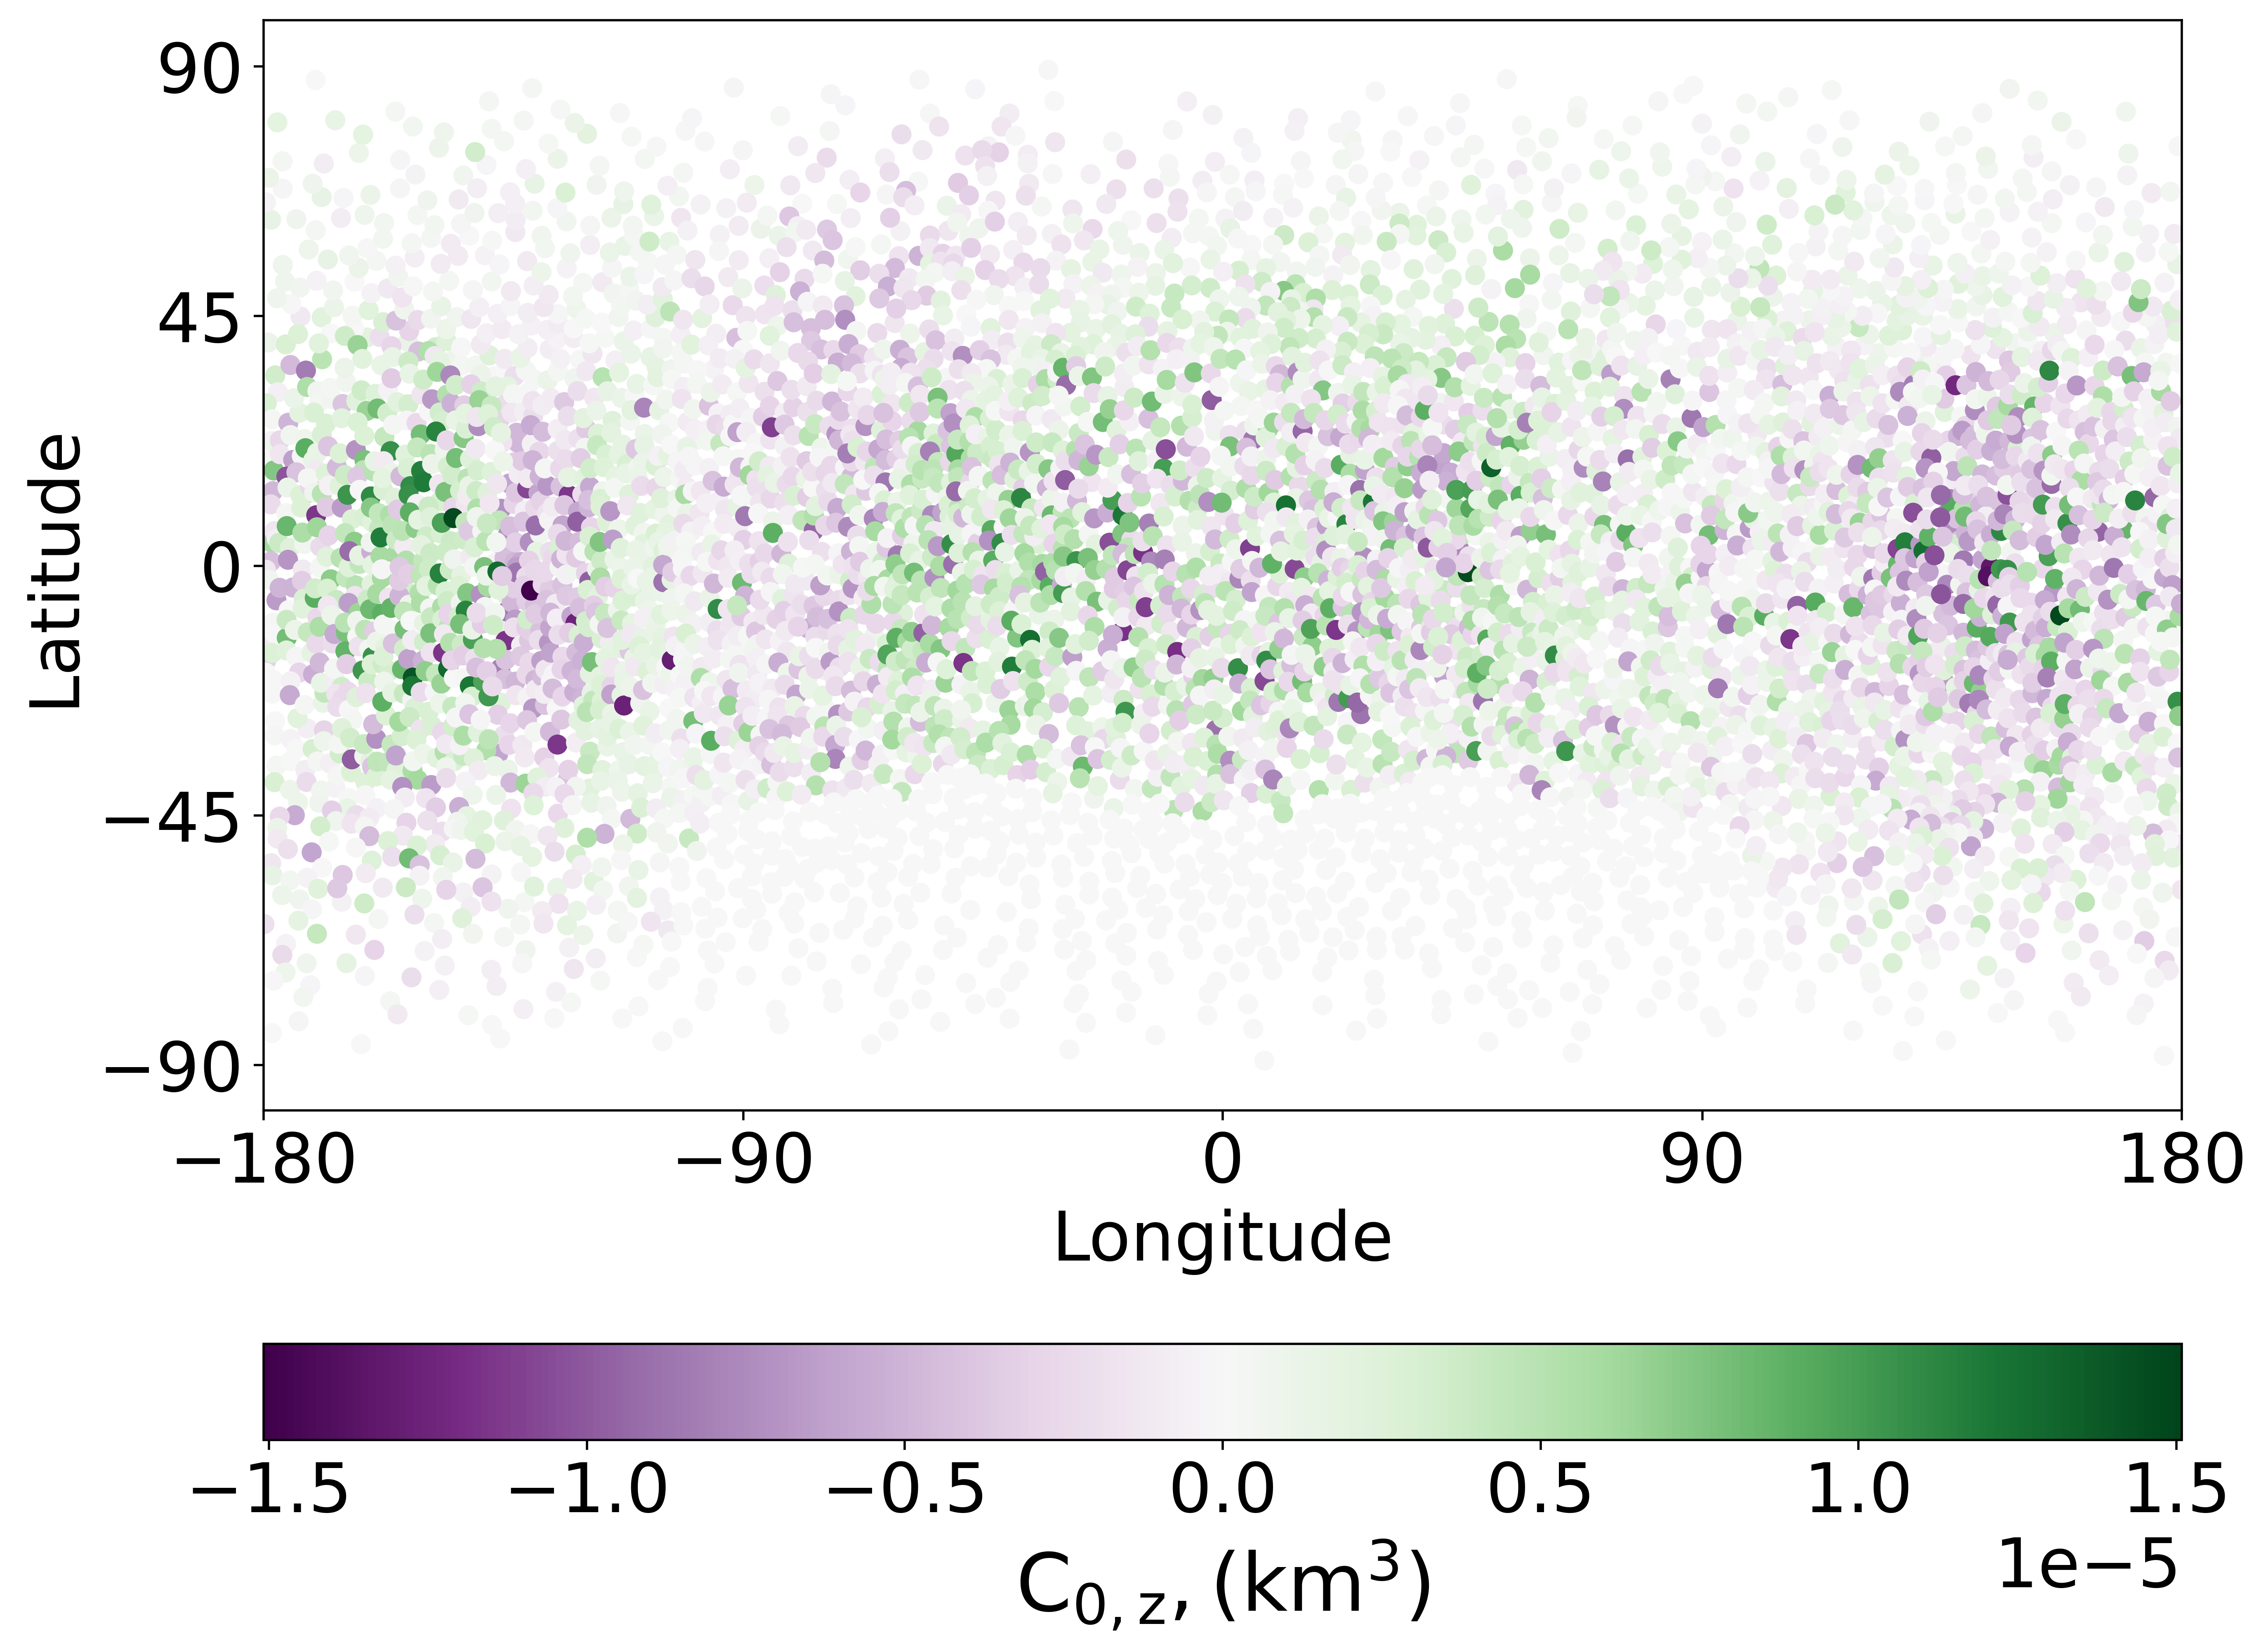
\includegraphics[width=\textwidth]{fig/itokawa_base_facet_yorp.png}
        \caption{Itokawa Surface YORP per facet}
    \end{subfigure}  
    \caption{First-order YORP spin coefficient variation per facet on Bennu and Itokawa}
    \label{fig:heatmaps}
\end{figure*}
The components that make up the probability density of the spin coefficient are considered in Eq.\ref{eq:5}.
\begin{equation}\label{eq:5}
    f(C_{0,z, total}) = f(C_{0,z, N})+f(C_{0,z, B})+f(C_{0,z, C})+f(C_{0,z, T})
\end{equation}
This is the probability density function associated with a specific value of YORP spin coefficient. It is a convolution of several source distributions of uncertainty: normal YORP as well as boulder-induced YORP, crater YORP, and tangential YORP. Each of these sources have their own factors influencing variability. In this analysis, we isolate the parameters that affect boulder-induced YORP, and discuss the associated contributions of crater YORP and tangential YORP for the entire probability density function. We also discuss the variation in normal YORP based on shape model resolution, and how to interpret different YORP spin torque results from low and high resolution models when the effect is extremely sensitive to small changes in surface normals. Delving deeper into boulder-induced YORP will then expand our capability to estimate YORP from an unresolved or poorly resolved surface that does not capture the resolution required to see the many small boulders. 

\begin{figure*}[t]
    \centering
    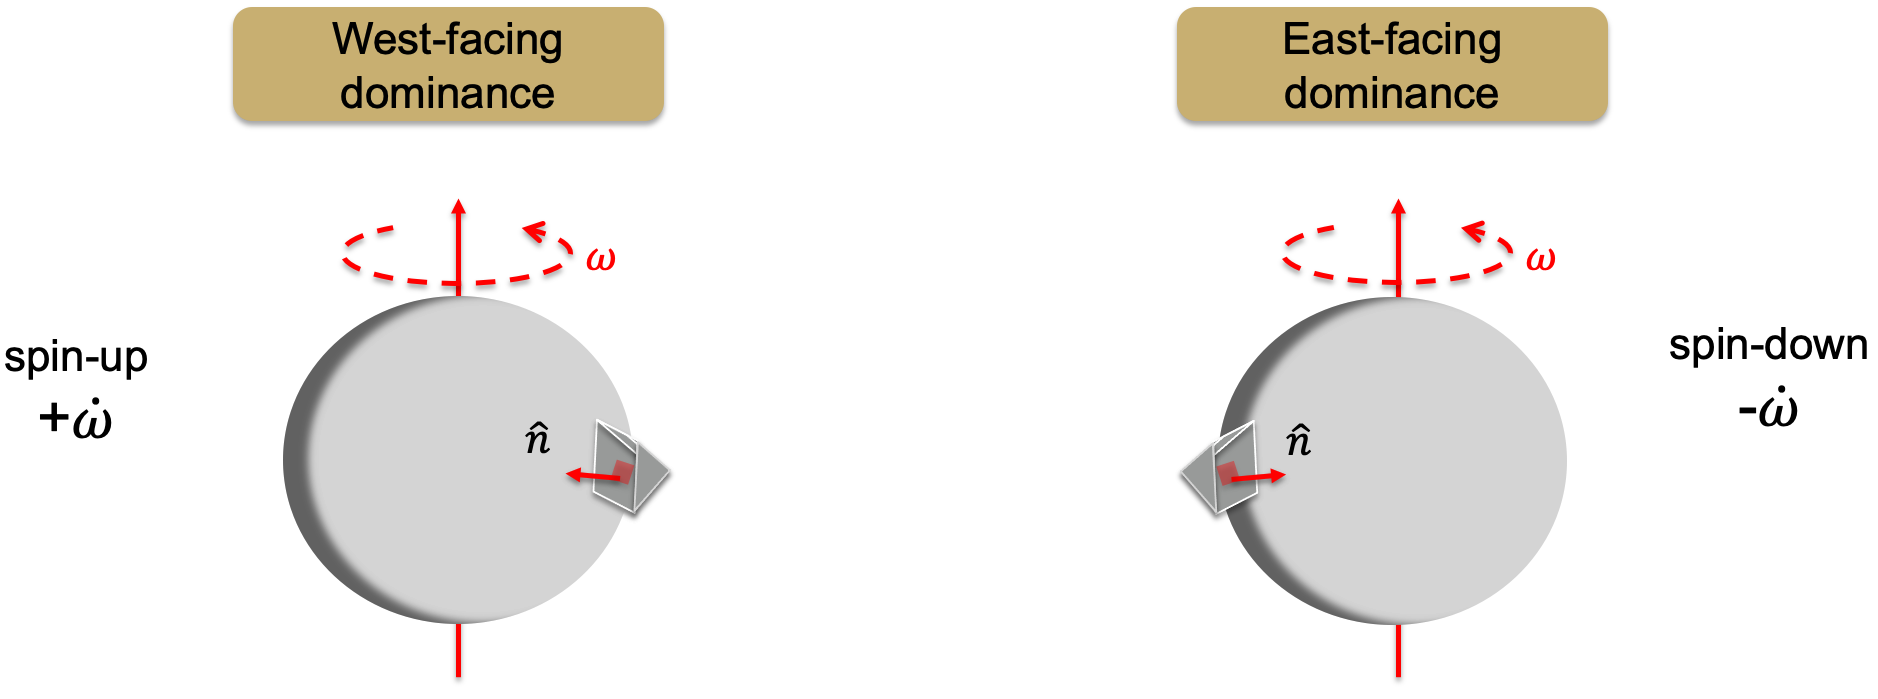
\includegraphics[width=0.85\textwidth,height=6cm]{fig/wedge_orientations.png}
    \caption{Wedge shape boulders provide asymmetry that induces YORP effect}
    \label{fig:wedges_on_asteroid}
\end{figure*}
\subsection{Boulder Shape}

In order to recreate the impact of boulders on an asteroid, we use an appropriate approximation of their shape. The nature of boulders leads to several options, but due to their variety there is no deterministic way to replicate all possible boulder shapes. The simple options are buried spheres \cite{Golubov2014}, walls \cite{Golubov2017}, or wedges \cite{Bottke2006}. Due to their directionality, wedges can direct YORP in preferential ways due to their longitudinal asymmetry. This activates YORP spin influence from a singular boulder whereas a symmetric boulder shape could not have an isolated effect on spin. In Fig.\ref{fig:wedges_on_asteroid}, it is shown how the leading or trailing larger face can impart the dominant YORP re-radiation in either the prograde or retrograde directions which determines the acceleration of the spin axis. 
We assume a Lambertian-scattering surface with the added dimension of boulder shapes at the size regimes expected for their respective parent body, from 10 cm to tens of meters. The bottleneck of this simulation and many simulations attempting realism is the computational burden due to resolution of details. This dilemma prompts the use of low-resolution shape models and low-resolution boulders. We justify this low-fidelity boulder shape by the fact that boulders have no predefined shape characteristics and can exist in many configurations and orientations, especially in micro-gravity environments. This wedge then becomes the isosceles prism shown in Fig. \ref{fig:prism}, which is scaled linearly with the diameter chosen for the boulder during simulation.


In this model, there is variation in both YORP re-radiation torque magnitude and direction depending on the local orientation on the surface. Aligning a perpendicular face directly tangential to the spin-axis maximizes the magnitude of re-radiation torque, while the geometry of the isosceles prism (or wedge) boulder creates a balance of one larger dominant face metered by two equal-sized faces whose off-axis dampen each other and their individual spin influence is diminished by a factor of $\sqrt{2}$.

\begin{figure}[H]
    \centering
    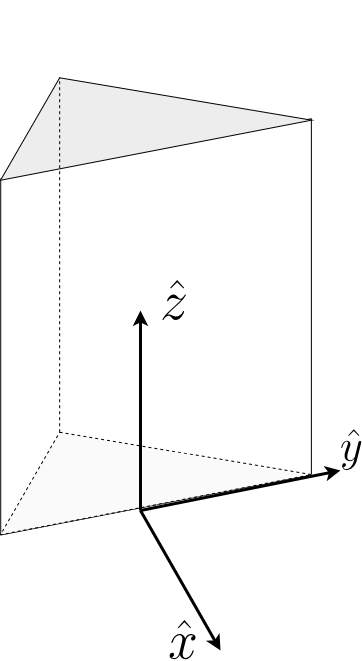
\includegraphics[width=0.25\textwidth,height=0.4\textwidth]{fig/prism.png}
    \caption{Boulder model with frame}
    \label{fig:prism}
\end{figure}

With this shape, we see a clear relationship between the dominant flat-face orientation and magnitude and sign of YORP spin contribution as we trace the changing ratio of west to east-facing surface area. The definition of orientation here is clockwise beginning with directly west-facing in the local asteroid surface frame, as shown in Fig. \ref{fig:rotate}. West and east here are defined by the body spin axis and direction; therefore a west-facing boulder is one where the $\hat{x}_B$ direction is aligned with the anti-spin direction. 

\subsection{Bennu and Itokawa Surfaces}

The asteroids selected to study YORP variability have been visited and characterized to a high level of detail. By detail, we refer to boulder counting studies which give actual numbers and sizes and locations of the discernible boulders at the time of spacecraft visitation. These asteroids are considered representative cases for their respective taxonomic classes. 
\\ \indent The near-earth asteroid Bennu is a prime example of a nearly spherical rubble pile classified as a B-type, or a subclass of the more general C-type (chondrite) bodies that exhibit darker surfaces and are made up of some of the oldest bare materials in the Solar System \cite{Lauretta2019}. With a largest diameter of 565 m, it is easily binned into the category of small bodies for which YORP torque dominates spin evolution. Examining a low-resolution model of Bennu with the addition of boulders on the surface can provide clues for how feature deformities can impact long-term evolution of both the surface itself and the contribution of the YORP effect to the dynamics. 
Secondly we examine the asteroid Itokawa, which is another member of the Apollo family of near-Earth objects. An S-type body with a spin period of 12.1 hours, this elongated ellipsoidal shape can be investigated to learn more about the difference in YORP contribution based on the lever arm potential of a feature. It has been found that a shift in center of mass of 15m could reverse the direction of YORP from spin-up to a spin-down state, further proving the sensitivity of the shape to the YORP effect \cite{Scheeres2008}.
Findings from the simulation of these population can be compared to the measured YORP parameters for these bodies, presented in Table \ref{table:asteroid_values}. While we have implemented the current simulations using a low-resolution surface models for modeling speed (5898 and 5714 facets for Bennu and Itokawa respectively), they exhibit the desired characteristics of general convexity and near-symmetry, or ellipsoidal non-convexity, which allows us to generalize the findings here for other bodies similar to either or somewhere between the two.
\begin{figure}[H]
    \centering
    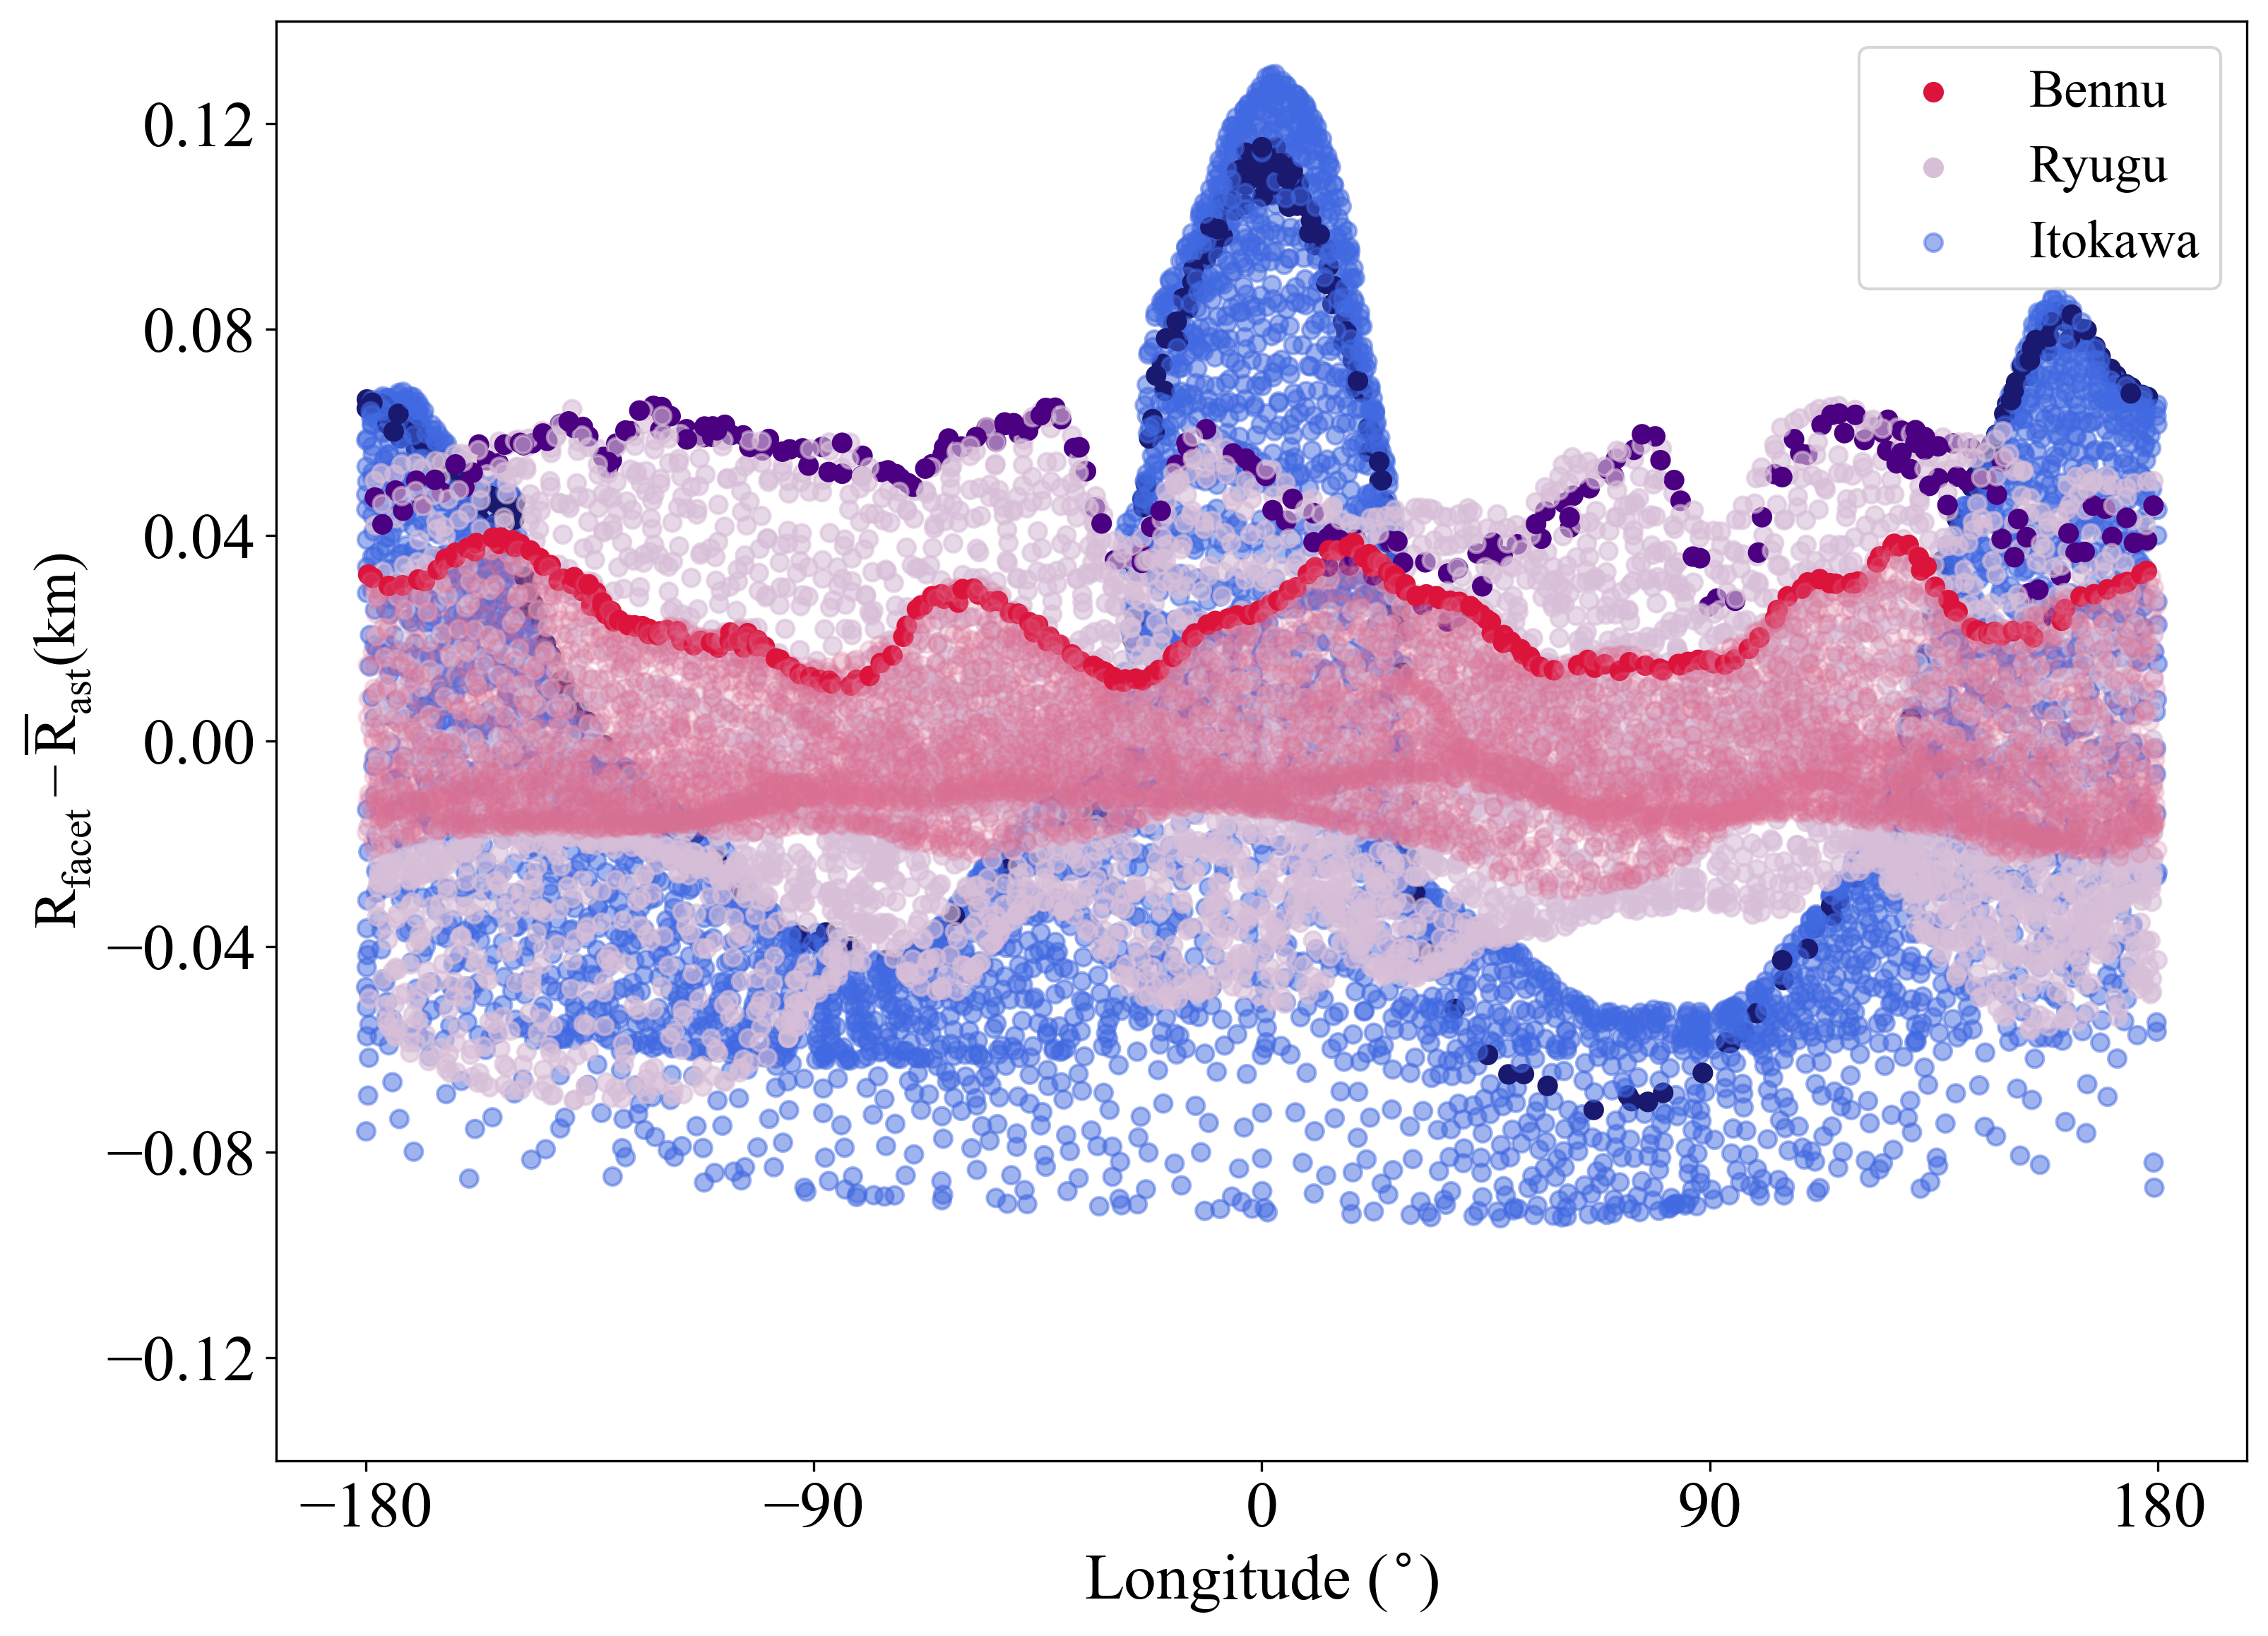
\includegraphics[width=0.4\textwidth]{fig/overlaid_shape_symmetry.png}
    \caption{Difference of per-facet distance from body center of mass and the average radius for three asteroid shape models: Bennu, Ryugu, and Itokawa. Darker points represent equatorial facets. Itokawa exhibits the greatest variation over longitude.}
    \label{fig:symmetry}
\end{figure}
The advantage of this approach is the availability of statistics on the body-specific boulder populations which could be shaped by specific material properties, cratering and regolith migration history, disaggregation or congregation during their formation events, or many other hypothetical and unobservable factors. The assumption of these physical processes is unnecessary because we use the current surface distribution directly. When it comes to future approaches simulating boulder motion, the material behavior and likelihood of dynamical outcomes must be approximated.


A common configuration found in near-earth asteroids is the roughly axi-symmetric spheroidal shape, such as Bennu and Ryugu. This is an ideal shape for examining the dependence of YORP on the latitude distribution of additional features because the total surface area is roughly equally distributed across all latitudes and longitudes. The results shown throughout this work will represent the possible YORP values for the spin component, $C_{0,z}(\delta_{s})$. It is important to note that a completely z-symmetric asteroid surface, such as a sphere or ellipsoid, would not experience YORP torque, but the addition of asymmetric boulders would induce a new torque by permuting the surface and adding asymmetry. 
In Fig.\ref{fig:symmetry}, the surface contours of three mapped asteroids are shown. The difference between the facet location and the mean radii is shown in longitude radius space to highlight the spread of each surface from a symmetric distribution, which would be a straight line. The asteroid Bennu shows the least amount of variance in facet distances, while Itokawa presents the most drastic variance in differences as it follows an asymmetric ellipsoidal pattern. Each shape consists of roughly 6000 facets each, and it is interesting to note that both Bennu and Ryugu have their largest radii along the equator, while Itokawa has surface points that reach farther and fall outside of the $2^{\circ}$ equatorial bound designated here.
\begin{table*}[b!]
    \renewcommand{\arraystretch}{1.5}

    \resizebox{\textwidth}{!}{
        \begin{tabular}{| c || c | c | c | c | c |}
        \hline
        \makegapedcells
        \textbf{Body} & \textbf{Dimensions} ($\mathbf{km}$) & \textbf{Surface Area} ($\mathbf{km^2}$)& \textbf{Spin Rate (rad/sec)} & \textbf{Calc.} $\dot{\omega}_{YORP}$, ($\mathbf{rad/day^2}$) & \textbf{Obs.} $\dot{\omega}_{YORP}$, ($\mathbf{rad/day^2}$) \\
        \hline 
        \hline
        \makegapedcells
        Bennu & (0.505,0.492,0.457) $\pm 0.002$ & $0.787 \pm 0.0004$ & \num{4.0613e-4} & \num{1.00378e-6} & $3.63 \pm$ \num{0.52e-6}\\ 
        \hline 
        \makegapedcells
        Itokawa & (0.535,0.294,0.209) $\pm 0.001$ & 0.3928 & \num{1.4385e-4} & \num{-2.03797e-5} & \num{3.54e-8}\\  
        \hline   
        \end{tabular}
        }
    \caption{Bennu's Properties and Itokawa's Properties}
    \label{table:asteroid_values}
\end{table*}

For the base models, we start with ~6,000 facet shape models of asteroids Bennu and Itokawa. We evaluate the YORP contribution to torque and obliquity of each facet based on its orientation in a $0^{\circ}$ obliquity sun angle over a single day. You can see the patterns of magnitude and sign in the shape model YORP distribution in Fig. \ref{fig:heatmaps}. You can see a divergence in magnitude of YORP and clustering on both of the two bodies. The base model that is used when examining the YORP contribution of boulders is significant as it determines how strong of a torque a feature can induce at a specific location. For reference at different points in this work, we see the observed YORP spin accelerations given in table \ref{table:asteroid_values}. This is gathered from observations of Bennu, \cite{Daly2020} \cite{Scheeres2016} \cite{Hergenrother2019}, and Itokawa, \cite{Fujiwara2006} \cite{Lowry2007} \cite{Breiter2009}. We also show the values of YORP spin acceleration calculated from our polyhedral facet YORP model. We focus on Bennu and Itokawa in order to observe the differences in boulder-induced YORP affect-potential on bodies with different levels of asymmetry and moments of inertia. Itokawa has a smaller surface area and is at a different dynamical state in it's YORP timescale versus Bennu, which has a larger surface area and larger observed YORP spin acceleration. We will discuss in Sec.\ref{discussion} why the calculation and observation values of YORP torque are different and how model resolution and natural sources of YORP uncertainty can be the cause.


\subsection{Boulder Population Studies on Bennu and Itokawa} \label{BP}

Size, location, and dominant re-radiation direction (which will be referred to as "west-pointing") all affect the YORP torqye of asteroid boulders. The morphology of boulders on a rubble-pile body can indicate formation and impact history or possible thermal fracturing. These different pathways to boulder presence change the expected size range for each body. As we examine the impact of boulders on the two candidate asteroid shapes, we take information from detailed boulder counting studies for sampling expected sizes. 


The spatial distribution of observed boulders is not uniform, depending on topographic valleys and gravitational potential \cite{Jawin2020}. It has also been suggested that since this distribution is highly dependent on the current state of surface evolution and regolith migration, it may be more appropriate to model distributions as fully uniform, or preferring shallower sloped regions or regions of low gravitational potential \cite{Jawin2022}. 
\begin{figure}[H]
    \centering
    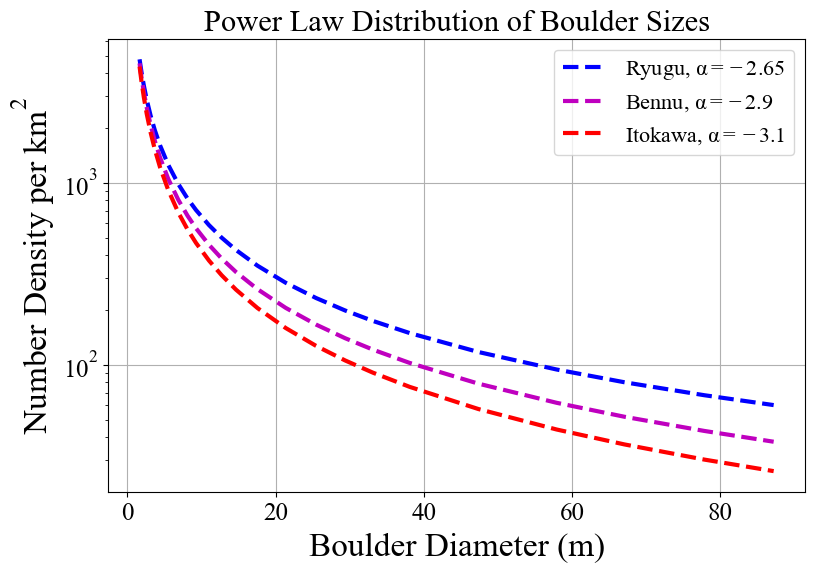
\includegraphics[width=0.45\textwidth]{fig/boulder_sizes_power_law.png}
    \caption{Cumulative number of boulders per square km}
    \label{fig:bs}
\end{figure}

\indent The sampled distributions for boulder sizes chosen in this work are shown in Fig.\ref{fig:bs}. This is the overlaid power law size relationship for three bodies, our two candidates and Ryugu for comparison. For the instantiation of a boulder population, we impose this power law on boulders randomly sampled across the surface. In reports on Bennu's surface characteristics, it is stated that it is "dominated" by boulders larger than 1m in diameter, and additionally we find hundreds above 10 m \cite{DellaGiustina2019}. 

\subsection{Applying a Simplified Thermal Model} \label{STM}

As mentioned in Delbo et al, the Yarkovsky effect is highly dependent on the surface material's thermal inertia.However, normal YORP is not \cite{Delbo2015}. The normal YORP effect modeled here is independent of thermal inertia and dependent on the shape, self-shadowing, and surface roughness causing re-radiation dispersion. However, in the theory of tangential YORP (TYORP), the propagation of thermal energy internally through a boulder is considered and thermal inertia is a factor. This type of YORP can impart a force tangent to the surface as the thermal differential between the initially sun-incident side of a boulder becomes equilibrated with the afternoon side, emitting additional radiation always in the pro-spin direction. Tangential YORP is metered by two qualities: the spin velocity and the boulder width. If an asteroid is spinning too fast or slow, it will either experience a constant temperature at the surface or exhibit thermal equilibrium with incident radiation (replicating Rubincam's approximation), respectively. For size limits, a boulder that is too thick will experience internal dissipation before the thermal energy can reach its opposite side. For the case where a boulder is too small or thin, the two sides can again be approximated as having instantaneous thermal equilibrium and the TYORP torque goes to zero \cite{Golubov2012}. 
\\ \indent As we consider the normal YORP (NYORP) for analyzing the addition of boulder shapes, we are primarily concerned with the geometric properties. This makes it more necessary to calculate accurate shadowing, and the thermal assumptions are simplified as a thermal lag as in Scheeres approximation. Further analysis will consider the addition of TYORP within its effective size regime, but our boulder population extends over a much broader range of radii. This will be seen in Sec. \ref{discussion}. 

\subsection{Polyhedral Facet YORP Evaluation}\label{PFYORPE}

The surface-wide normal YORP torque is calculated on a facet-by-facet basis, allowing for granularity in the surface geometry and a functional approximation for absorption and remission vectors. A shape model made up of vertices, facets, and facet normal directions can be used for the entire basis of YORP calculations in all solar latitude orientations. The most intensive and necessary calculation is the visibility function, which determines where, when, and for what duration self-shadowing occurs on the body. This visibility coefficient is used to linearly scale the torque contribution from a specific facet. For this formulation, and computational efficiency, boulders here are not considered as shadow-inducing features. 
Force imparted on a facet element of a body is a combination of the normal and transverse elements of the YORP effect. Using terms specifically for solar irradiation, we reference the indexed force equation for the $i$th facet of an asteroid \cite{Scheeres2007}:

\[
    \mathbf{f}_i (\mathbf{\hat{u}}) = -\big[ {\rho s(2\mathbf{\hat{n}}_i \mathbf{\hat{n}}_i - \mathbf{U}) + U} \cdot \mathbf{\hat{u}}\mathbf{\hat{u}} \cdot \mathbf{\hat{n}}_i  
\]
\begin{equation}
    + a_2\mathbf{\hat{n}}_i \mathbf{\hat{n}}_i \cdot \mathbf{\hat{u}}\big] H_i(\mathbf{\hat{u}})  A_i,
\end{equation}

where it is shown that the force due to solar radiation scales linearly with the area of the facet, moderated by the illumination function $H_i(\mathbf{\hat{u}})$. We apply this equation to evaluate the YORP contribution of a given boulder based on it's surface area and facet orientations, assuming that the entire surface and every feature of the body has 0$\%$ specularity, a reflectivity coefficient of $0.05$, and exhibits ideal Lambertian scattering behaviors. 
Each boulder shape is analyzed for the possibility of being shadowed by surface contours, which is required in order to accurately consider the sun-rise and sun-set angles, as well as the horizon occultations that may occur throughout the day if a boulder inhabits a shadowed valley. The shape is iterated over to calculate shadowing of each facet until all of the shadowing angle bounds are found, $\lambda_r$ and $\lambda_s$. The components of YORP torque are then calculated from the orientation, thermal assumptions, shadowing bounds and visibility function, and facet area. For a non-zero obliquity $\epsilon$, the body will wobble between the $[-\epsilon,+\epsilon]$ bounds of the equivalent solar latitude, so the overall YORP torque from the normalized coefficient must consider the entire range of possible illumination angles. 

\section{Analysis of boulder impact on YORP spin torque}\label{analysis} %section 4

Bennu's collection of boulders is one representative sample of size range, placement, and global impact that we will be presenting here to examine the relationship between additional surface features and total YORP spin. It is interchangeable with any asteroid boulder population that has been characterized, or theoretical boulder distributions. We define total YORP in this context as:
\begin{equation}
    T_{YORP} = T_{NYORP} + T_{BoYORP}
    \label{eq:ugh}
\end{equation}
This is the combination of the base surface YORP, or normal YORP, and the additional effect of added boulders on the surface, boulder-induced YORP (boYORP). These are both calculated via the simple thermal model and geometric analysis of sun illumination angle and duration. It is boYORP that we are examining with statistical variability, assuming that we know our surface to the degree that the shape model is accurate. When discussing the percent impact of an individual boulder, this means the ratio of the singular boulder's normal YORP versus the total YORP of the surface and every boulder. We also reiterate the focus on just the first-order spin torque component of YORP described by proxy with the $C_{0,z}$ Fourier coefficient. The impact of tangential YORP experienced by boulders will be discussed in later sections. 


\subsection{Power Law Distribution of Boulder Size}
We expect to see a probability of any size boulder within the bounds of minimum and maximum observed size to be characterized as follows. 

\begin{equation}
    p(x) \propto x^{-\alpha}
\end{equation}
The power $\alpha$ is characterized by boulder counting studies. In computation, the distribution is bounded by physical minimum size. A formula for sampling random numbers in this distribution is derived in Clauset et al. \cite{Clauset2009}.

\begin{equation}
    x = x_{min}(1-r)^{-1/(\alpha-1)},\qquad r \in \mathbf{U}(0,1)
\end{equation}
This provides a random selection of x, the boulder diameter, selected from the bounded power law distribution of sizes. 


The entire boulder population sample set, spanning the range of surface area and orientation, is roughly 2.95 million individual features. This number is arrived at by generating one boulder model on each facet of a low-resolution model, which equates to 1 boulder per 130 $m^2$ of surface area, and varying the orientation with a resolution of $\frac{2\pi}{500}$ for all possible angles. This constitutes the full sample set $n$, where we then choose $k$ number of boulders at random to form one instance of an asteroid surface distribution. The variable $k$ is set to match the expected feature density of the body. This is done $p$ times until statistical significance is confidently ensured, typically 500 times to give 500 possible asteroid surface instantiations per body. The power law size distribution of boulders is imposed after choosing location and orientation, which is possible to apply in post-processing due to the linear approximation of the YORP coefficient as a function of boulder surface area. We assume that scaling a boulder in this way will not change shadowing orientations that were found and the boulders themselves are not considered to impart shadows themselves. In the imposition of these probability distributions, we are left with Gaussian equatorial bias in latitude due to the larger equatorial surface area, as well as a uniformly sampled orientation angle. The size distribution is biased towards smaller diameter boulders as one would expect from real surfaces. We can define the binomial coefficient allowing for resampling as follows:

\begin{equation}
    \begin{pmatrix} n+k+1\\ k\end{pmatrix} = \frac{(n+k+1)!}{k!(n+1)!}.
\end{equation}

In this formulation, $n$ is the 2.95 million initial boulder set, while $k$ is the 5000 boulders selected to form a single possible observation of a boulder distribution. This number is astronomically large, meaning that we will see unique placement and orientation combinations in each sample set. We select this set $p = 500$ times to gather information about the significance of boulder size, location, and orientation over many samples. We go on to explain the relationship between boulder size and it's individual level of significance in the evaluation of the YORP torque over an entire asteroid.

To analyze the statistical likelihood of boulders contributing greatly to YORP, we select $500$ sets of $5000$ boulder models per body. 


An impactful boulder can be defined as contributing in magnitude to the YORP torque felt by the asteroid past a specified threshold, defined as a percent of the asteroid YORP experienced with boulders. However, this is measured in absolute value and in large sets of boulders, one finds frequent complements in boulders contributing to both spin acceleration and spin slowing. The rapid spin-up attributed to one large west-facing boulder can be muted by many small east-facing features. 
\begin{figure*}[t!]
    \centering
    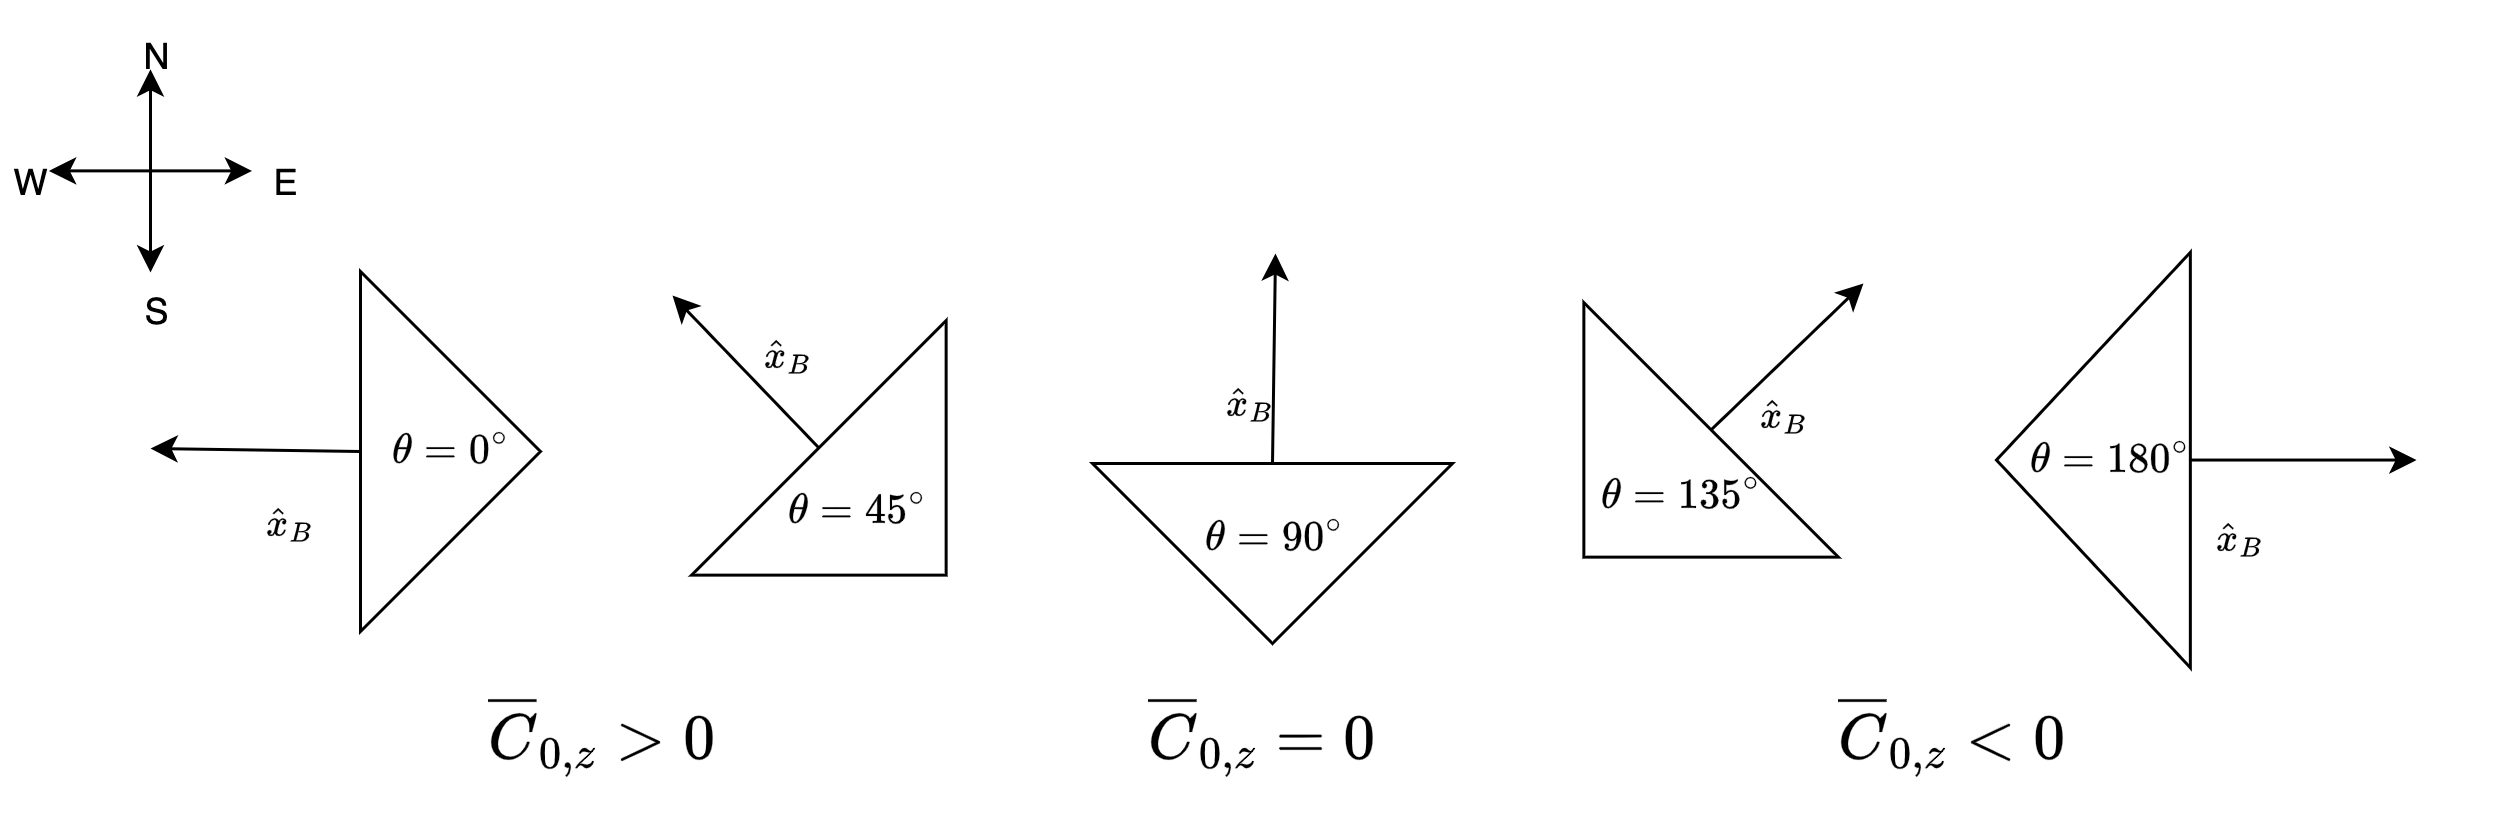
\includegraphics[width=0.8\textwidth]{fig/rotating_wedge.png}
    \caption{Orientation of Prism Boulder Rotating from West to East, from $0$ to $\pi$}
    \label{fig:rotate}
\end{figure*}

\subsection{Uniform Distribution of Boulder Location}\label{location}
There is no explicit dependence on latitude for a boulder to maximize its contribution to YORP torque. For many spherical-like rubble piles, the spin moment encourages movement of material to the equator. As we analyze an oblate spheroidal shape, this relationship is clear. Longer torque arms at the equator maximize the contributions of YORP torque from boulders at this latitude. From the profile of surface distances shown in Fig. \ref{fig:symmetry}, it is clear that the largest lever arms are about the equator for Bennu and Itokawa. This is not true for every shape; therefore we investigate the range of distance from spin pole for the population of impactful boulders.

We begin with a distribution of equal sized boulders over a discretized shape model. The shape has been divided into facets of roughly equal area. Due to the fitting of equal triangles over ellipsoidal or spherical shapes, there are more boulders at equatorial latitudes than polar. In further analysis, we are able to bias the selection of boulders towards either preference, and we will show how that affects the YORP torque accordingly. We chose this discretization to allow for uniform sampling over the surface area of the body, leveraging the vectorization already contained within the base shape model.


\subsection{Uniform Distribution of Boulder Orientation}

The distribution of torque as a factor of orientation is symmetric about zero and it can be shown that the dominant directionality of boulder re-radiation is self-limiting when enough boulders are sampled. However, we can depend on the variation in size to maximize or minimize the orientation dominant direction in asymmetric ways for random individual boulders which is what will provide an overall YORP torque. Some locations are sloped or shadowed such that they only allow a boulder to re-radiate in one direction, but that is captured in our YORP calculations as we vary every boulder over all orientations. Boulders tangent to the spin pole are also able to exist in intermediate positions that meter the total torque effects in a sinusoidal relationship, see Fig. \ref{fig:sine}. Here we calculate torque directly from the spin coefficient for a single value of true anomaly. 
\begin{equation}
    T_{boYORP} = P(R) C_{0,z}
\end{equation}
The torque here is related to the spin coefficient by the solar pressure at $R$, the distance of the body from the sun. The sign of the YORP torque relationship shown varies over three cycles for an entire rotation, which shows that, for this specific isosceles prism shape, we observe a high amount of variability. Future studies may investigate more realistic boulder shapes and the impact of variance in orientation on the YORP torque. 

The equation-of-fit corresponds to the Fig. \ref{fig:sine}. We examine a 10 m diameter boulder placed at the equator with the underlying facet normal aligned to the body $-\hat{x}$ axis. The torque is calculated as it rotates with angle $x_{rot}$. The fit is a sum of sine function with coefficients provided in table \ref{coeffs}. This fit provides an r-value of 0.995 to the torque function of this specific boulder size, placement, and normalizing parameters corresponding to the asteroid Bennu's orbit.
%here I provide the sine equation and table
\begin{equation}
    \bar{T}_{fit} = a_1\sin(b_1 x_{rot} + c_1) + a_2\sin(b_2 x_{rot} + c_2) + ... 
\end{equation}

%insert a table here with 4 columns and 4 rows
\begin{table}[H]
    \centering
    \begin{tabular}{|c|c|c|c|}
        \hline
        Fit Coefficients &$a_i$ & $b_i$ & $c_i$ \\
        \hline
        1 & 0.2177 & 2.887 & 1.896 \\
        2 & 0.06712 & 0.4036 & 0.276 \\
        3 & 0.09053 & 2.599 & -0.3521 \\
        4 & 0.01993 & 5.052 & -1.813 \\
        \hline
        Parameters & $\phi$,  $W m^{-2}$ & $R_{ast}, km$  & P(R), $kg km^3 s^{-2}$ \\
        \hline
         & 1400& 0.244 & 5.55e-3  \\
         \hline
    \end{tabular}
    \caption{Coefficients for the sum of sines fit of boulder YORP for single boulder at equator and aligned to body $-\hat{x}$ axis.}
    \label{coeffs}
\end{table}
The dominant re-radiation orientation of a boulder is highly stochastic therefore the uncertainty due to the orientation is uniformly distributed. Our choice in shape conditions the final distribution of boulder-induced YORP with its sinusoidal function resulting from the rotation of a standing isosceles prism. 

\begin{figure}[H]
    \centering
    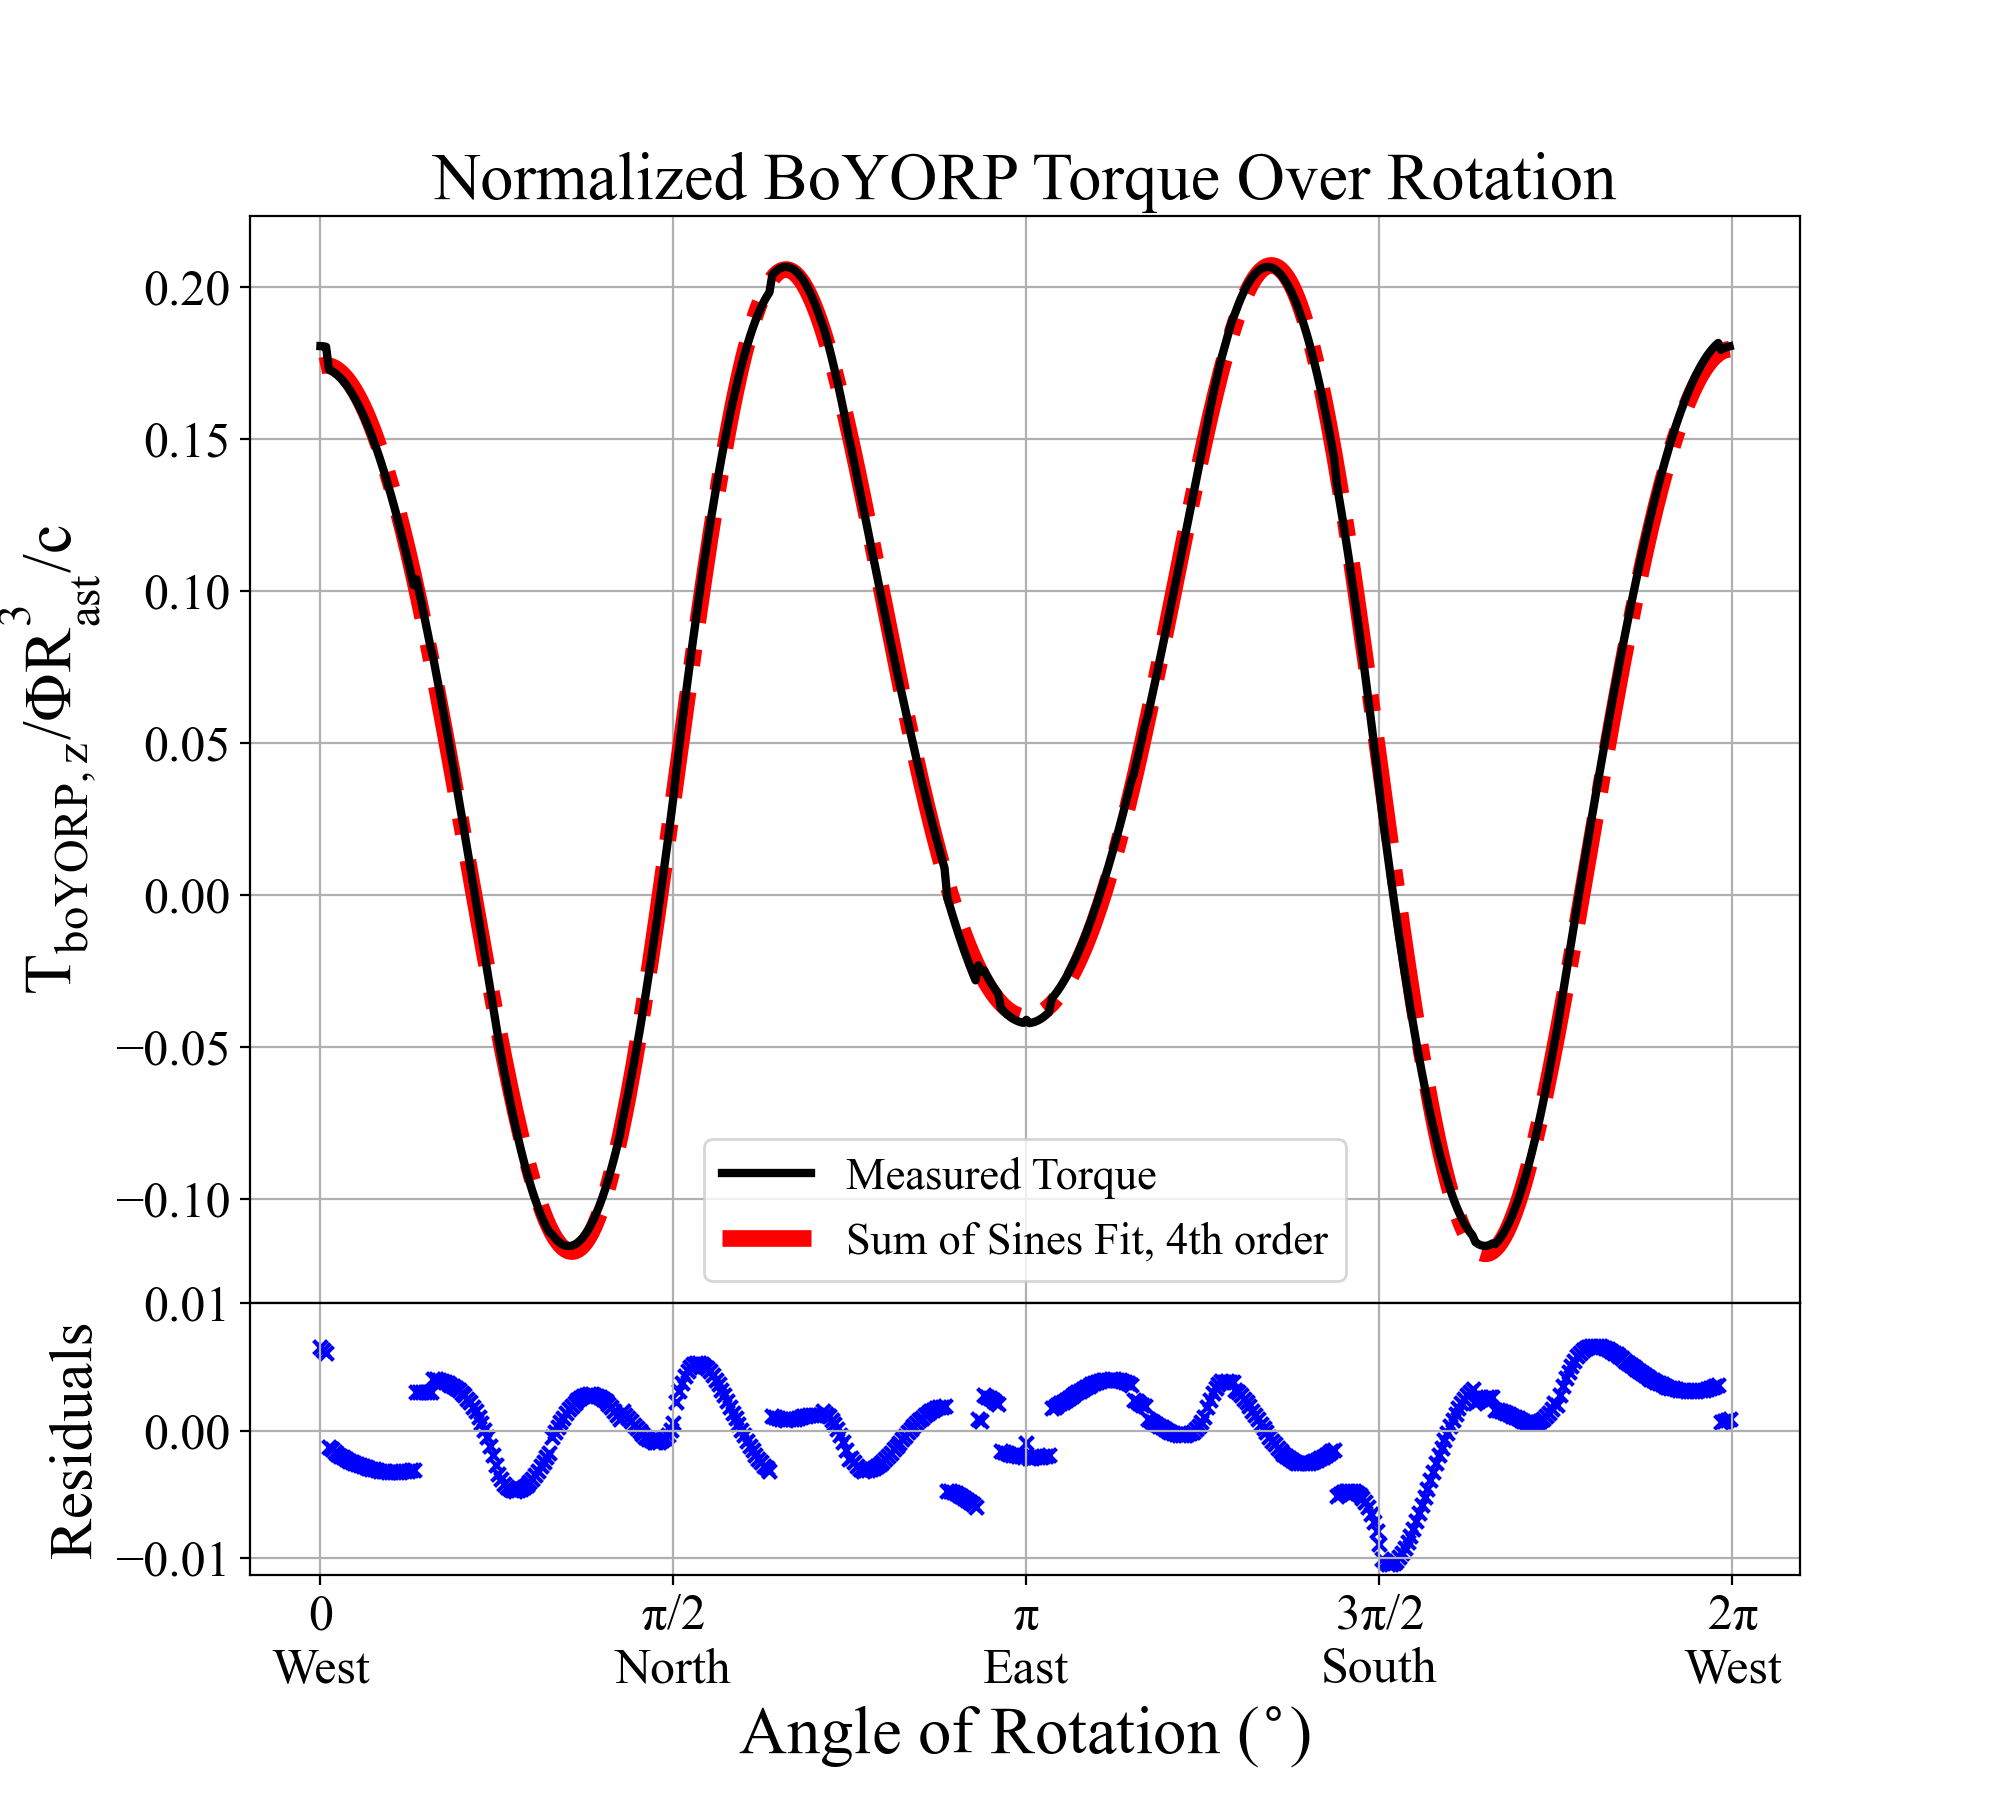
\includegraphics[width=0.45\textwidth]{fig/rotation_plot_one_equator_boulder.png}
    \caption{Sinusoidal relationship of boulder orientation to YORP torque. Asymmetric boulder at equator and perfectly tangent to spin pole}
    \label{fig:sine}
\end{figure}


\subsection{Overall Uncertainty Distribution}

We are uncertain about the distribution of boulder sizes on an asteroid and how far it may deviate from perfect power law behavior, but the latest observations have corroborated a power-law like distribution. We can sample this power law uniformly many times to find a variance in the typical population size. We assume uniform distribution of the small boulders, as has been reported in previous work \cite{DellaGiustina2019}. However, the local slope of the body, which is only known to the level of mapping detail, can affect the distribution of large boulders that have higher potentials. The orientation of the boulder that allows for the maximum vector of YORP torque is completely random in most natural cases. We propose biasing events and examine the outcome of this in the discussion, but for the natural statistics, we must assume that this is uniformly random. Collectively, we can characterize the uncertainty of boulder-induced YORP by these qualities: the resolution of the surface, the stochasticity in boulder sizing based on age and type, the likelihood of concentrations of boulders in valleys versus uniform spacing, and the orientation which directly affects the sign of the YORP torque. 

We can model the uncertainty due to the sampling of the power law as the uncertainty in the slope parameter, $\alpha$. This is a measure of the steepness of the power law. The uncertainty in the slope parameter is given by the variance, $\sigma_{\alpha}$. Since the power law itself is analytically an asymptotic function, it's variance is a function of the sample size, $n$, and is proposed to be asymptotically Gaussian. The maximum likelihood estimator of the slope parameter is given by the formula to follow \cite{Clauset2009}.  
\begin{equation}
    {\sigma^2}_{\alpha} = \frac{{\alpha-1}^2}{n}
\end{equation}
The other source of uncertainty in the power law is in the minimum diameter. This can be equally described in the uncertainty of image resolution and resulting shape model resolution, so we will not consider it as a separate source of uncertainty.

Since we derived our sampled data from optical measurements, we can incorporate the uncertainty from pixel resolution. The OSIRIS-REx PolyCam instrument achieved a 0.33 m per pixel resolution, while it's MapCam imaged down to 1.1 m per pixel. These are the sources for our boulder-counting data sets \cite{DellaGiustina2019}. As the boulder sizes are reported, we can assume that they are only accurate to 0.33 m. As for Itokawa, the mapping camera aboard Hayabusa2 was able to capture 0.7 m per pixel in their high resolution mapping campaign \cite{Saito2006}. This is the data used to report boulder size and location distributions \cite{Michikami2008}. These data sources inform the bounds on our certainty of size for each respective boulder distribution.
The low-resolution shape model of Bennu that is applied in this work is a degraded surface approximation from the SPC version 20 model presented by Barnouin. Similarly, we have down-processed the SPC model of Itokawa by Gaskell \cite{Gaskell2006}. This degradation was required for computational speed of the Monte Carlo methods.
We will show in future sections that this is not be concerning due to the ratio of YORP torque imposed from boulders less than 1m. However, as it pertains to uncertainty as a whole, we can only expect our model to have a surface YORP resolution comparable to a 25m facet. This resolution does change the calculations of YORP for the base shape, and we compare the low and high resolution YORP values in section \ref{discussion}. However, we use this rough approximation in order to place boulders in locations that are reasonably distributed across the body. The boulders themselves are much higher resolution and we examine their values independent of base shape resolution.

%%%%%%%%%%%%%%   RESULTS %%%%%%%%%%%%%%%%%%%%%%%%%%%%%%%


\section{Bennu Results}\label{bennu}

\subsection{Total Boulder Impact}
Each individual global simulation case was evaluated for YORP spin contribution per boulder, which included calculating rise and set longitudes as well as shadowing bounds. These boulders were randomized in location, orientation, and size along their individual distributions. In Fig.\ref{fig:cases_w_boulders}, we show the collective results from 500 randomly chosen samples.
\begin{figure}[H]
    \centering
    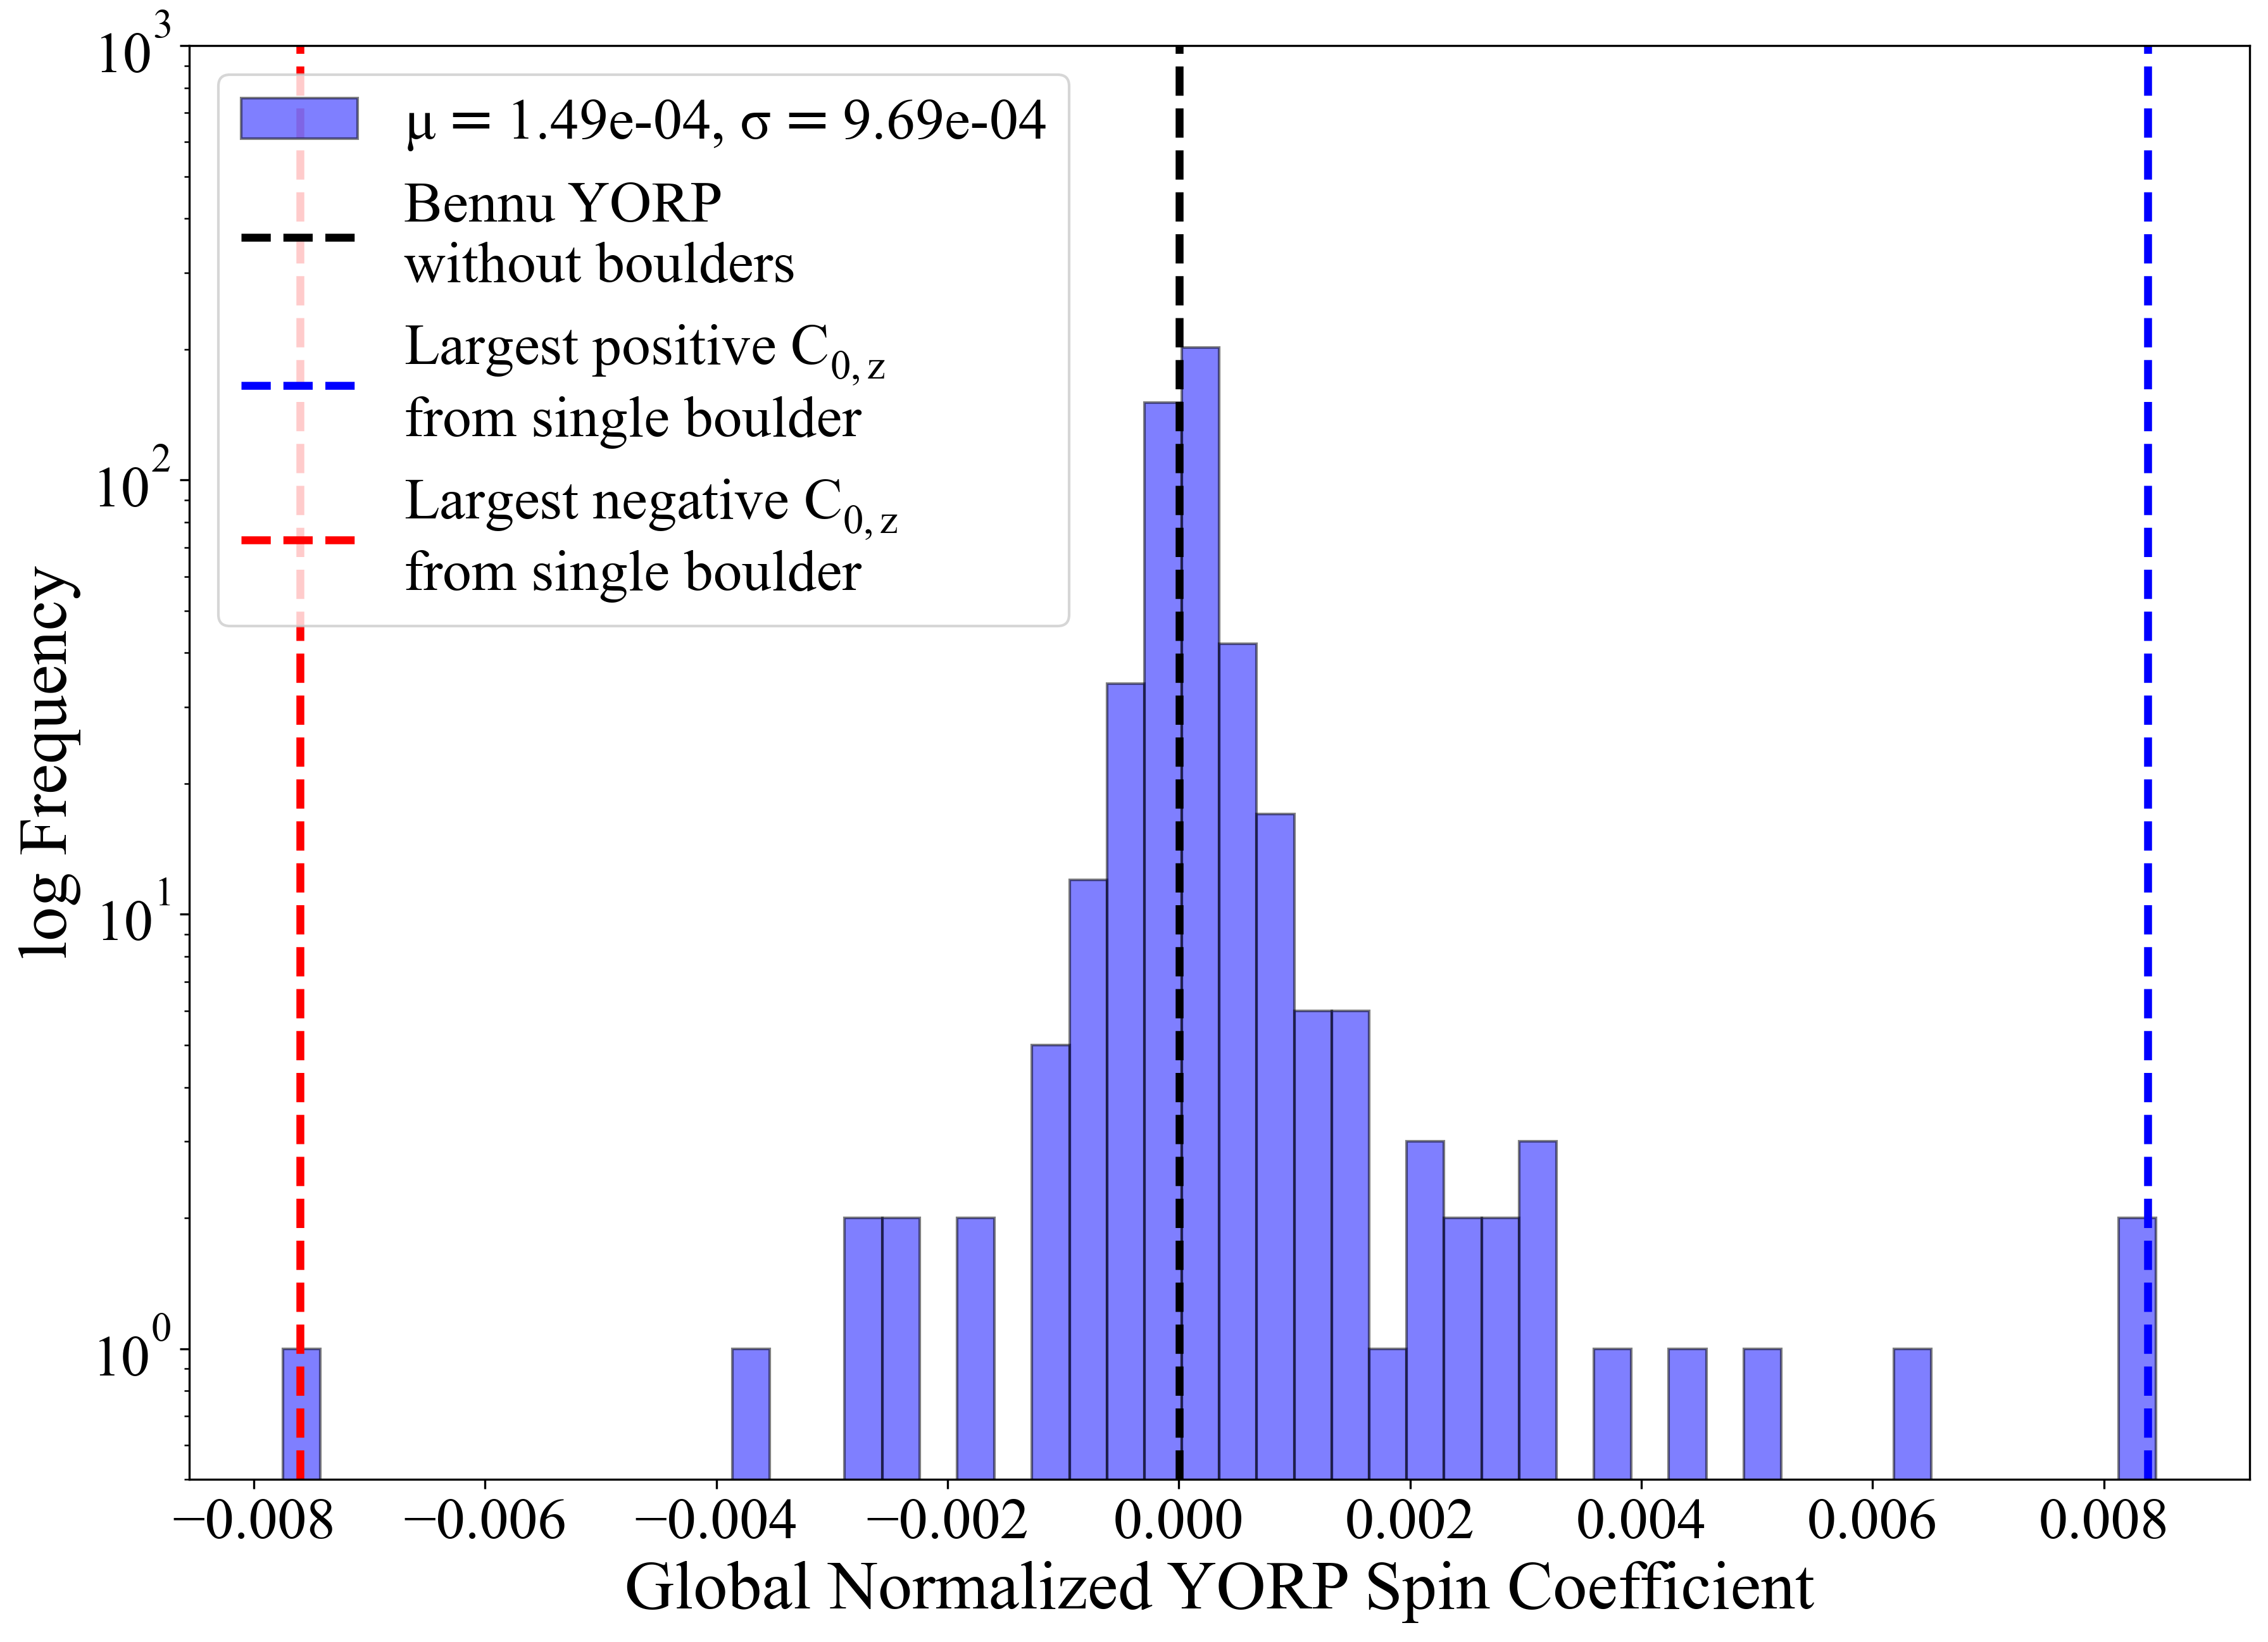
\includegraphics[width=0.49\textwidth]{fig/bennu_comparison.png}
    \caption{Frequency distribution of YORP with 500 random boulder populations for Bennu}
    \label{fig:cases_w_boulders}
\end{figure}

The addition of boulders can affect the global YORP up to 135 times the magnitude of the original value for the asteroid Bennu. This is equivalent to the contribution of a single large well-placed boulder, contributing a YORP spin coefficient value of \num{1.77e-4} compared to the Bennu base shape YORP coefficient,\num{1.324e-6}. This largest magnitude spin coefficient from a single boulder is at $-20.26^{\circ}$ latitude, and has a diameter of 54 m, the highest bound of the size distribution and roughly equivalent to the boulder BenBen. While the existence of these large contributors is rare in most of the global population cases, their influence is necessary to consider when quantifying the variability in YORP. Throughout the next section, we will show the trends related to boulders that are considered large contributors to YORP, at a proportion of 1\% of global YORP spin torque. 

\subsection{Large Influence Boulder Parameters}
\begin{figure}[H]
    \centering
    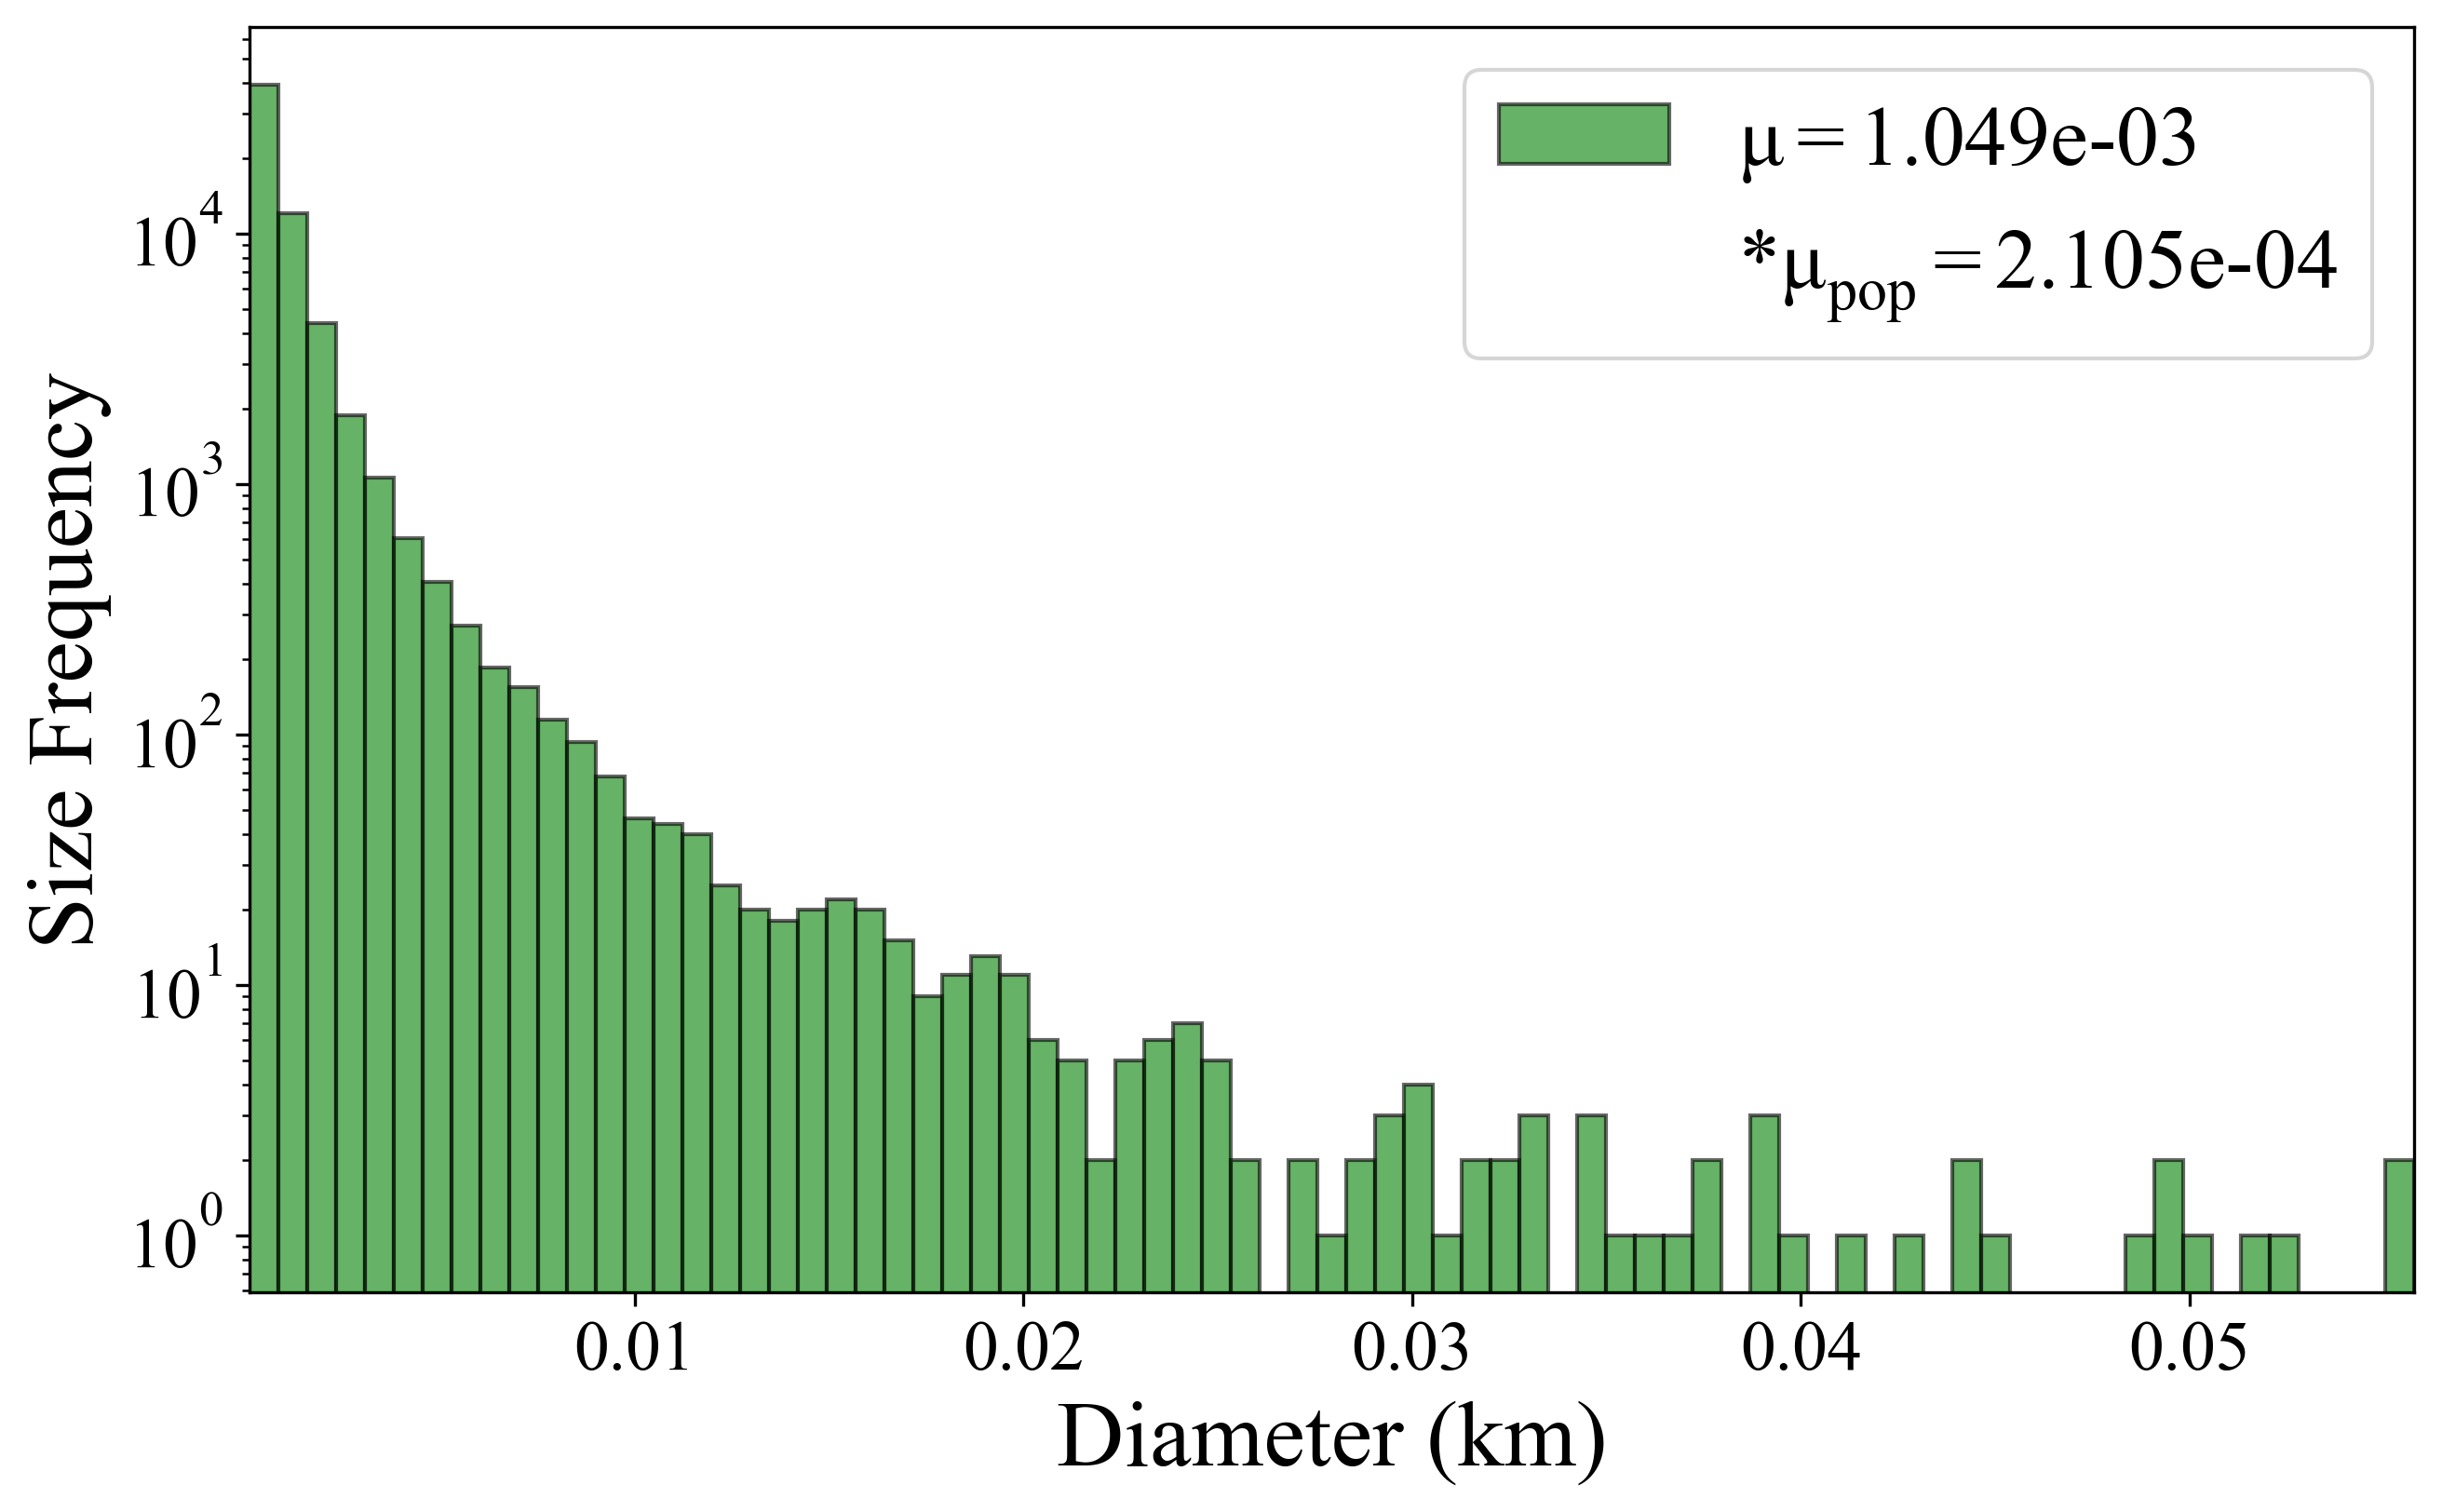
\includegraphics[width=0.45\textwidth]{fig/bennu_impact_size_new.png}
    \caption{Size distribution and mean diameter of boulders where $C_{0,z,i} > 1\%$ on Bennu}
    \label{fig:percents}
\end{figure}
\begin{figure*}[t!]
    \centering
    \begin{subfigure}[t]{0.49\textwidth}
        \centering
        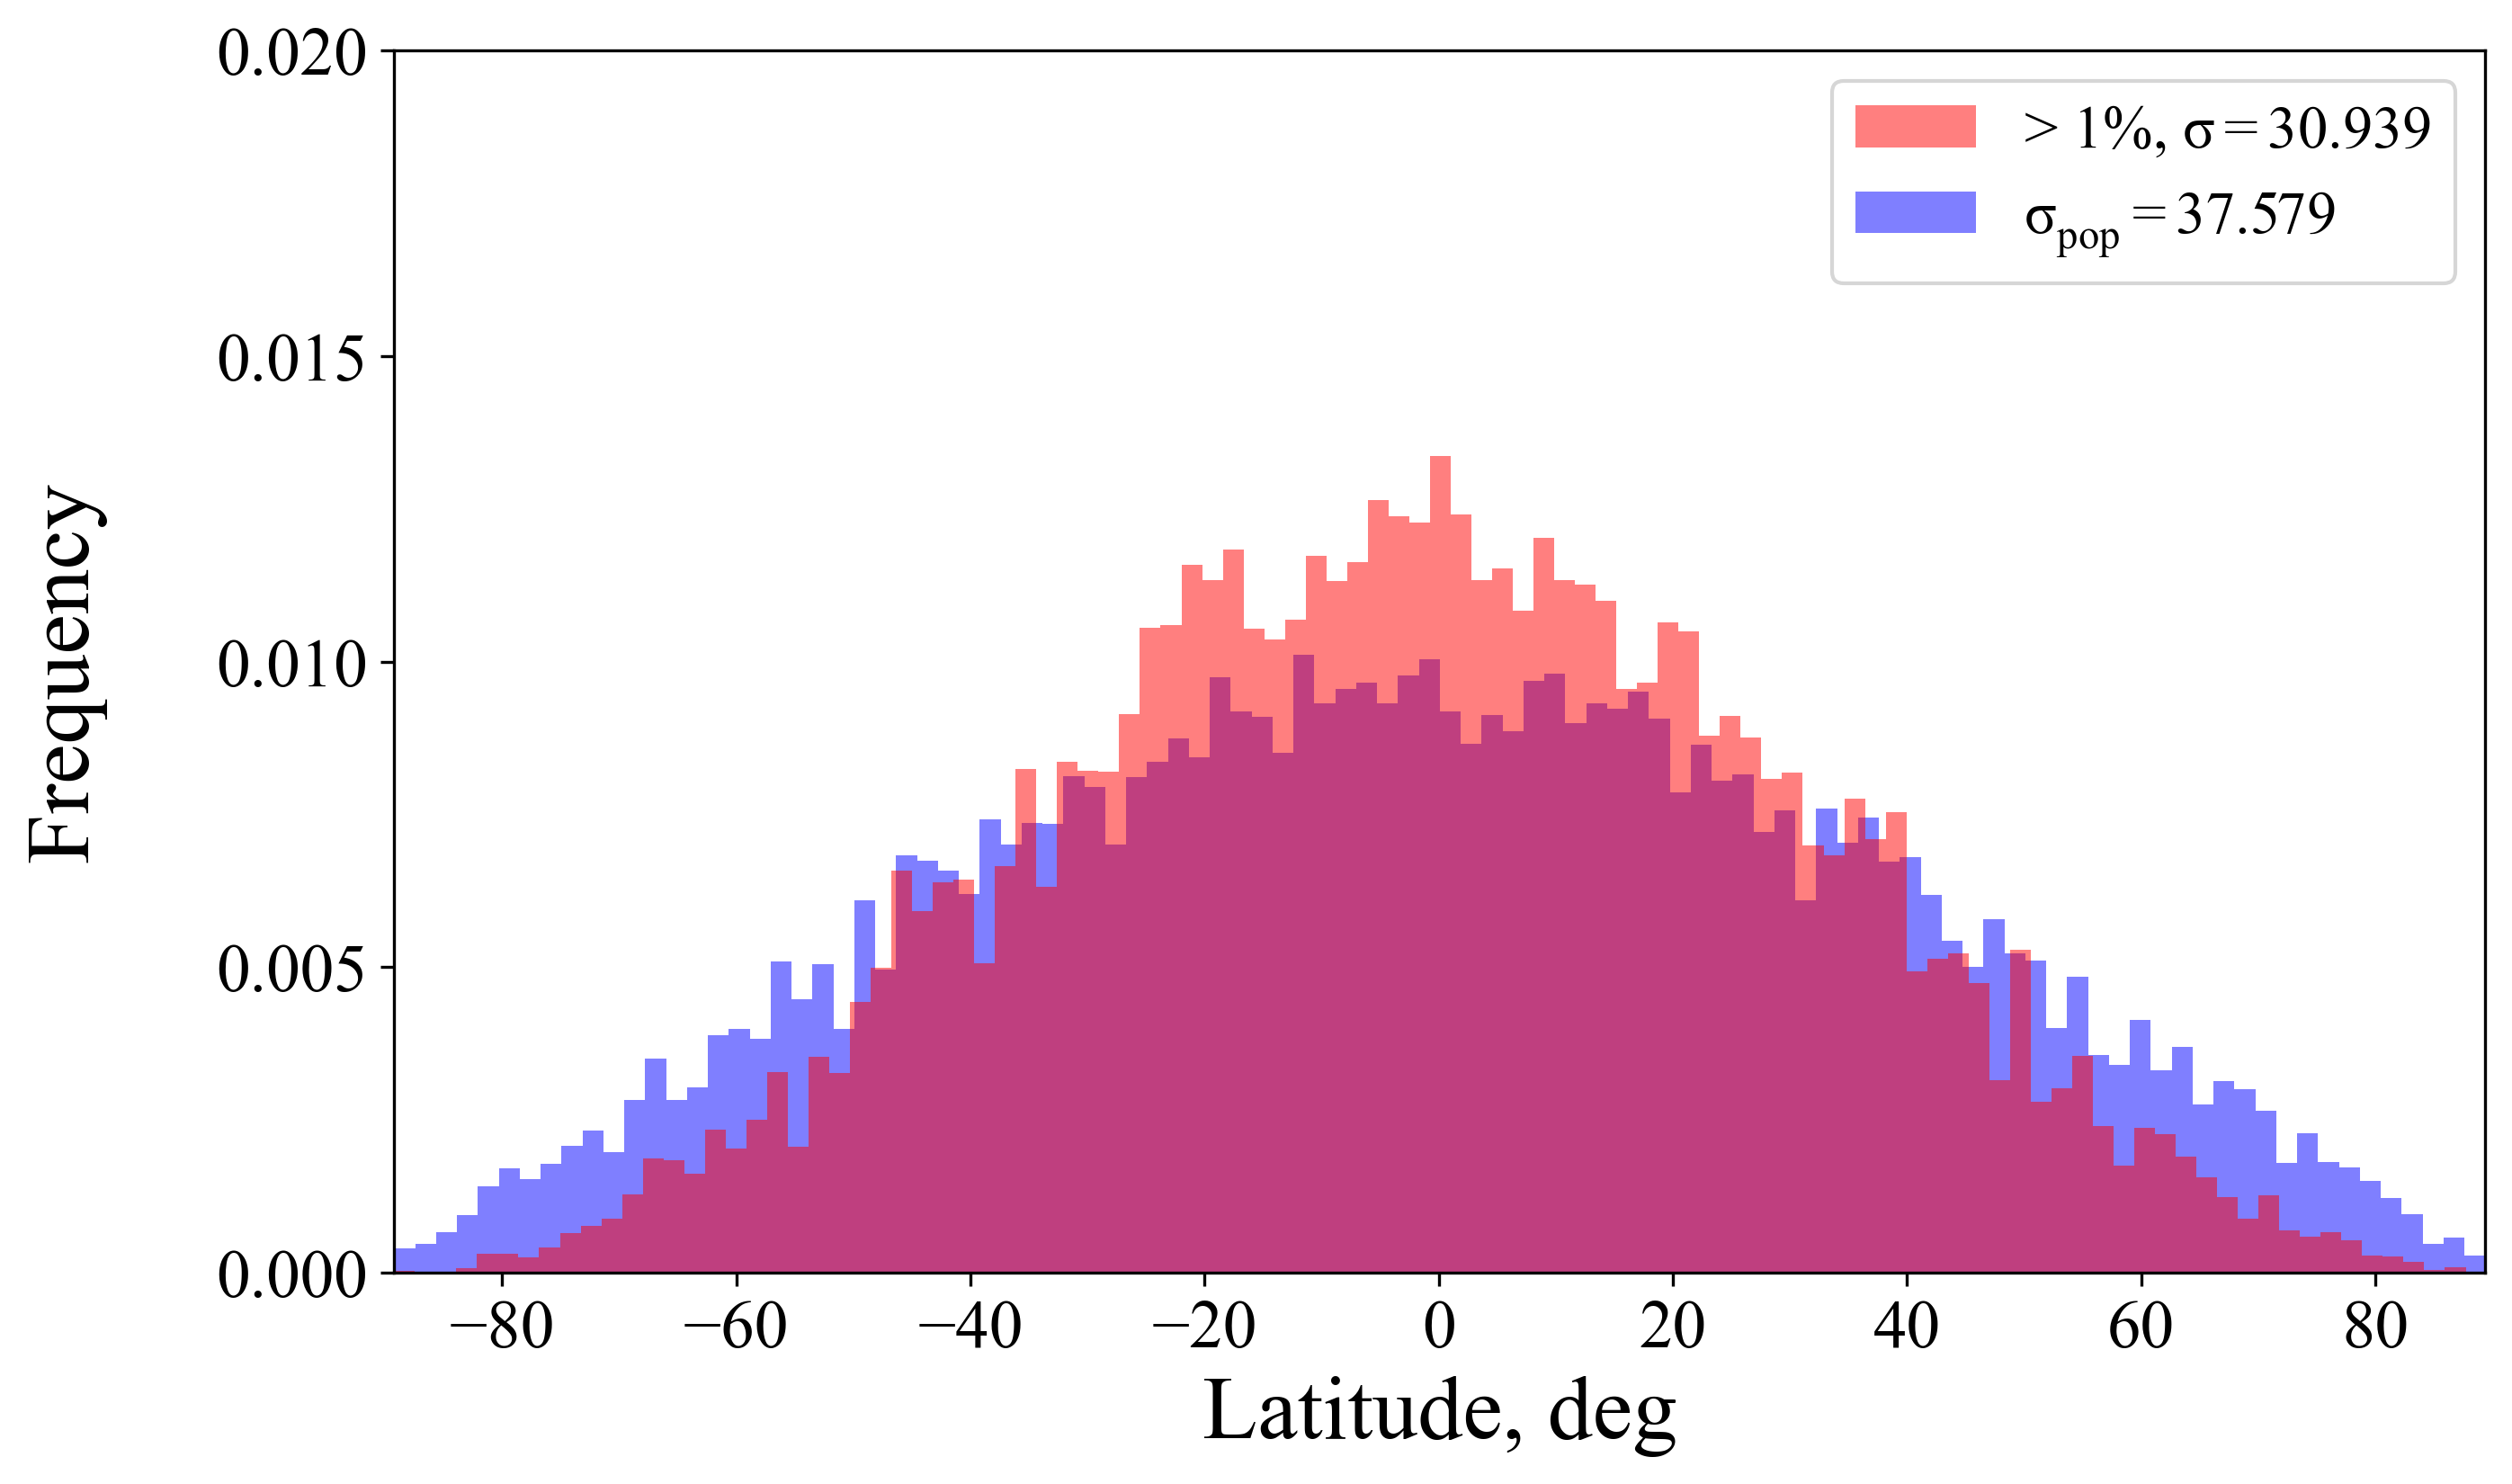
\includegraphics[width=\textwidth]{fig/bennu_impact_location_new.png}
        \caption{Latitude distribution of impactful boulders and the entire population set}
        \label{fig:latitudes}
    \end{subfigure}
    \hfill
    \begin{subfigure}[t]{0.49\textwidth}
        \centering
        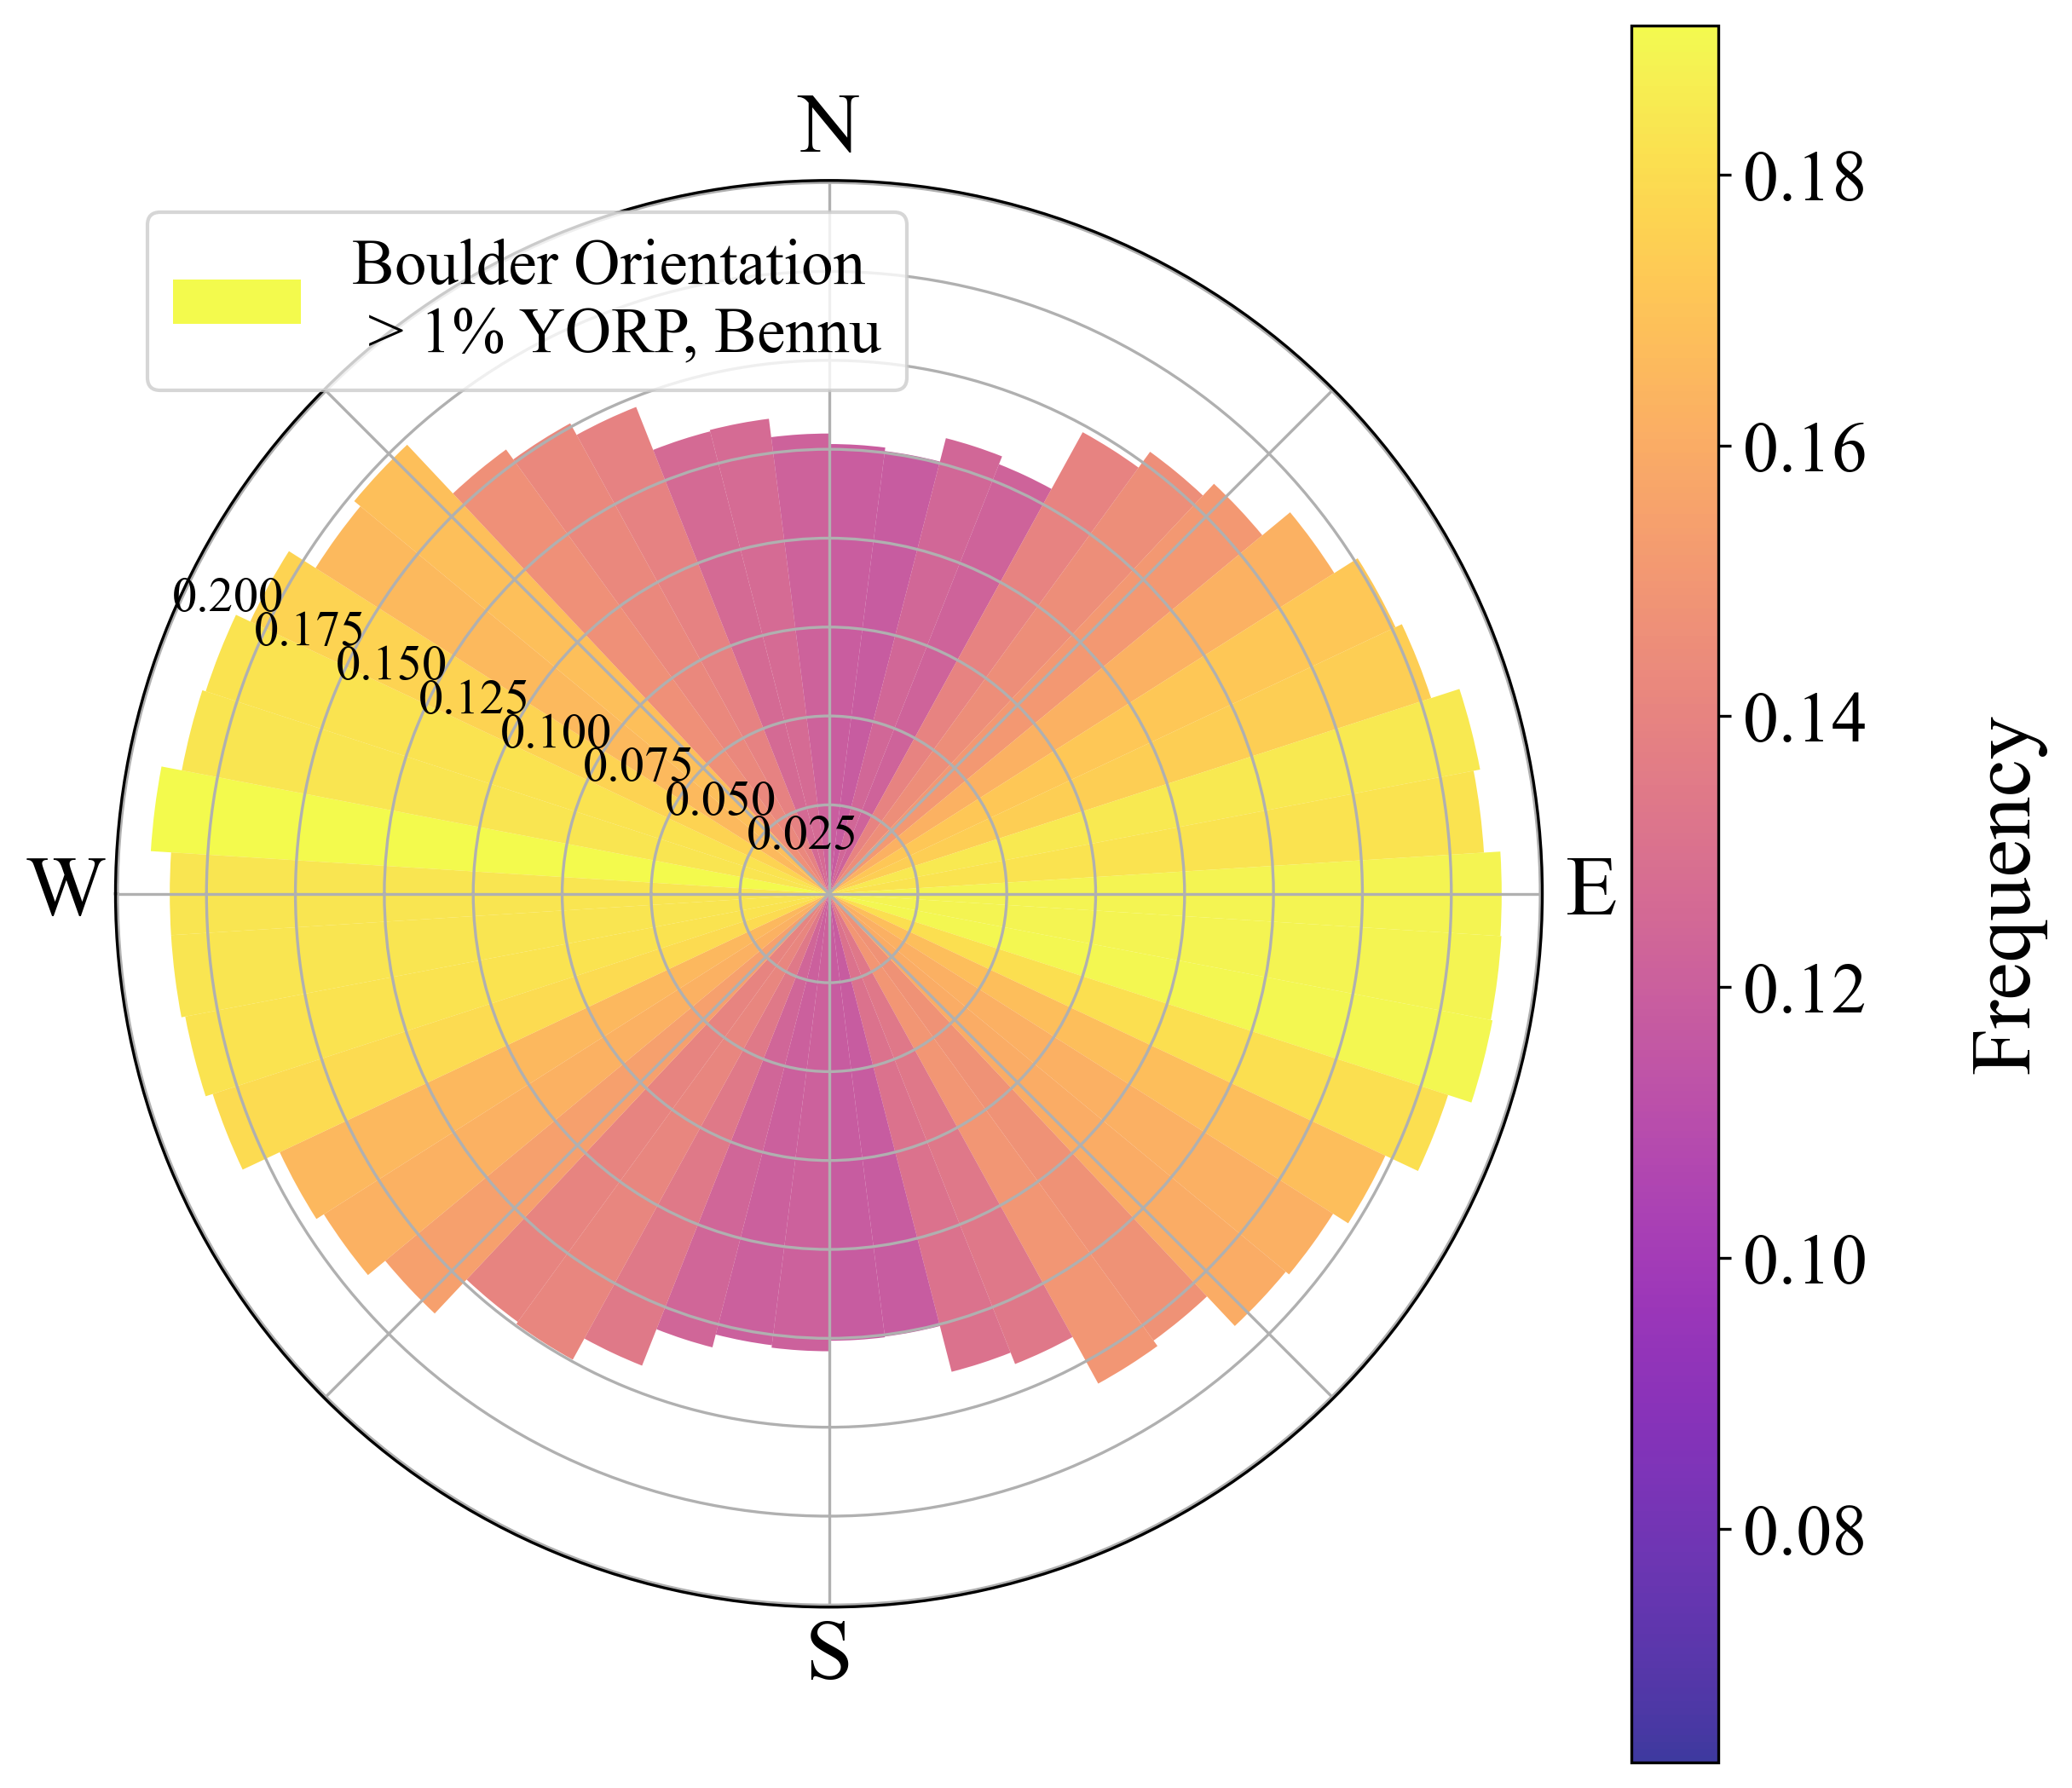
\includegraphics[width=0.75\textwidth]{fig/bennu_impact_orient_new.png}
        \caption{Frequency of boulder orientation for the impactful boulder population on Bennu}
        \label{fig:orientation}
    \end{subfigure}
    \caption{Bennu distribution comparison of normalized frequencies of boulder latitude and orientation in the > 1\% YORP spin coefficient boulder population.}
    \label{fig:bennu_results}
\end{figure*}

\subsubsection{Size Comparison}
When analyzing the population of boulders that contribute to greater than $1\%$ of total torque, there is a clear trend. The mean diameter of an impactful boulder, at this scale, is roughly 5 times larger than the population average, as shown in Fig. \ref{fig:percents}. The minimum and maximum of this subset of boulders considered impactful ranges from the population minimum, 10 cm, to the population maximum, 54 m. This subset contains just 1.2\% of our large population. Note that this encompasses 500 instances of a "Bennu" surface with boulders, consolidated together and individually compared to Bennu's base shape YORP torque plus boulders to find the subset of boulders that provide over 1\% additional torque. With these results, it is expected that each instance of a boulder population could contain 60 individual boulders that change torque for the entire body more than 1\% of the global value. However with further consideration of the uniform distribution of positive and negative torque boulders due to orientation, this effect may be self-dampened as number of boulders increases. 


\subsubsection{Location: Equatorial Trend}
The distribution of impactful boulders has a stronger density about the equator of Bennu, as shown by the standard deviation of the distributions in Fig. \ref{fig:latitudes}. When comparing the full resampled population to the ones filtered for having greater than 1\% global YORP spin influence, the standard deviation is 18\% smaller. This can also be described by comparing the relative frequency at the equator. In the unfiltered population, it is expected to find a boulder at the equator with a normalized frequency of 0.01. This increases to 0.014 when examining only the boulders that contribute over 1\% to YORP spin. This highlights that Bennu is oblate, seeing as the most impactful boulders congregate around the equatorial region. The average boulder distance from the z-axis on Bennu is 127 m, compared to its largest equatorial radius of 282 m, which aligns with expectations for oblate spheroid geometry.


\subsubsection{Orientation Bias: West or East} 


Once more, filtering for large YORP contributors while considering another influential parameter, we clearly see in our oval-shaped direction distribution that there is a higher frequency of boulders pointing more west or more east, in spin-delta maximizing orientations. This is emphasized by our selection of a boulder geometry which can maximize torque in preferential orientations: specifically, the alignment of the largest flat face pointing direction with the spin pole tangent.

The boulders that point north or south, at angles $\pm \pi/2$ away from local west, are depleted in this subset. In the coming sections we show the impact of biasing boulders towards the west at greater than uniformly random proportions. This will show the global impact of orientation dominance that may arise from biasing events such as spin-related weathering or longitudinal ridge formation. 


%%%%%%%%%%%%%%%%%%%%%%%%%%%%%%%%%%%%%%%%%%%%
\section{Itokawa Results}\label{itokawa}

\subsection{Total Boulder Impact}
When examining the variation in Itokawa surface simulations with boulders added, a smaller extent of variability is found versus our previous model. Shown in Fig.\ref{fig:itokawa_all_cases}, the strongest variation from Itokawa's natural calculated YORP value is 12 times larger, where Itokawa's base normalized coefficient is $-0.0036$ and the largest magnitude case of difference is $-0.0423$. The variability in this data set arises from the distributions applied to the predetermined boulder factors of size, orientation, and location. 
\begin{figure}[H]
    \centering
    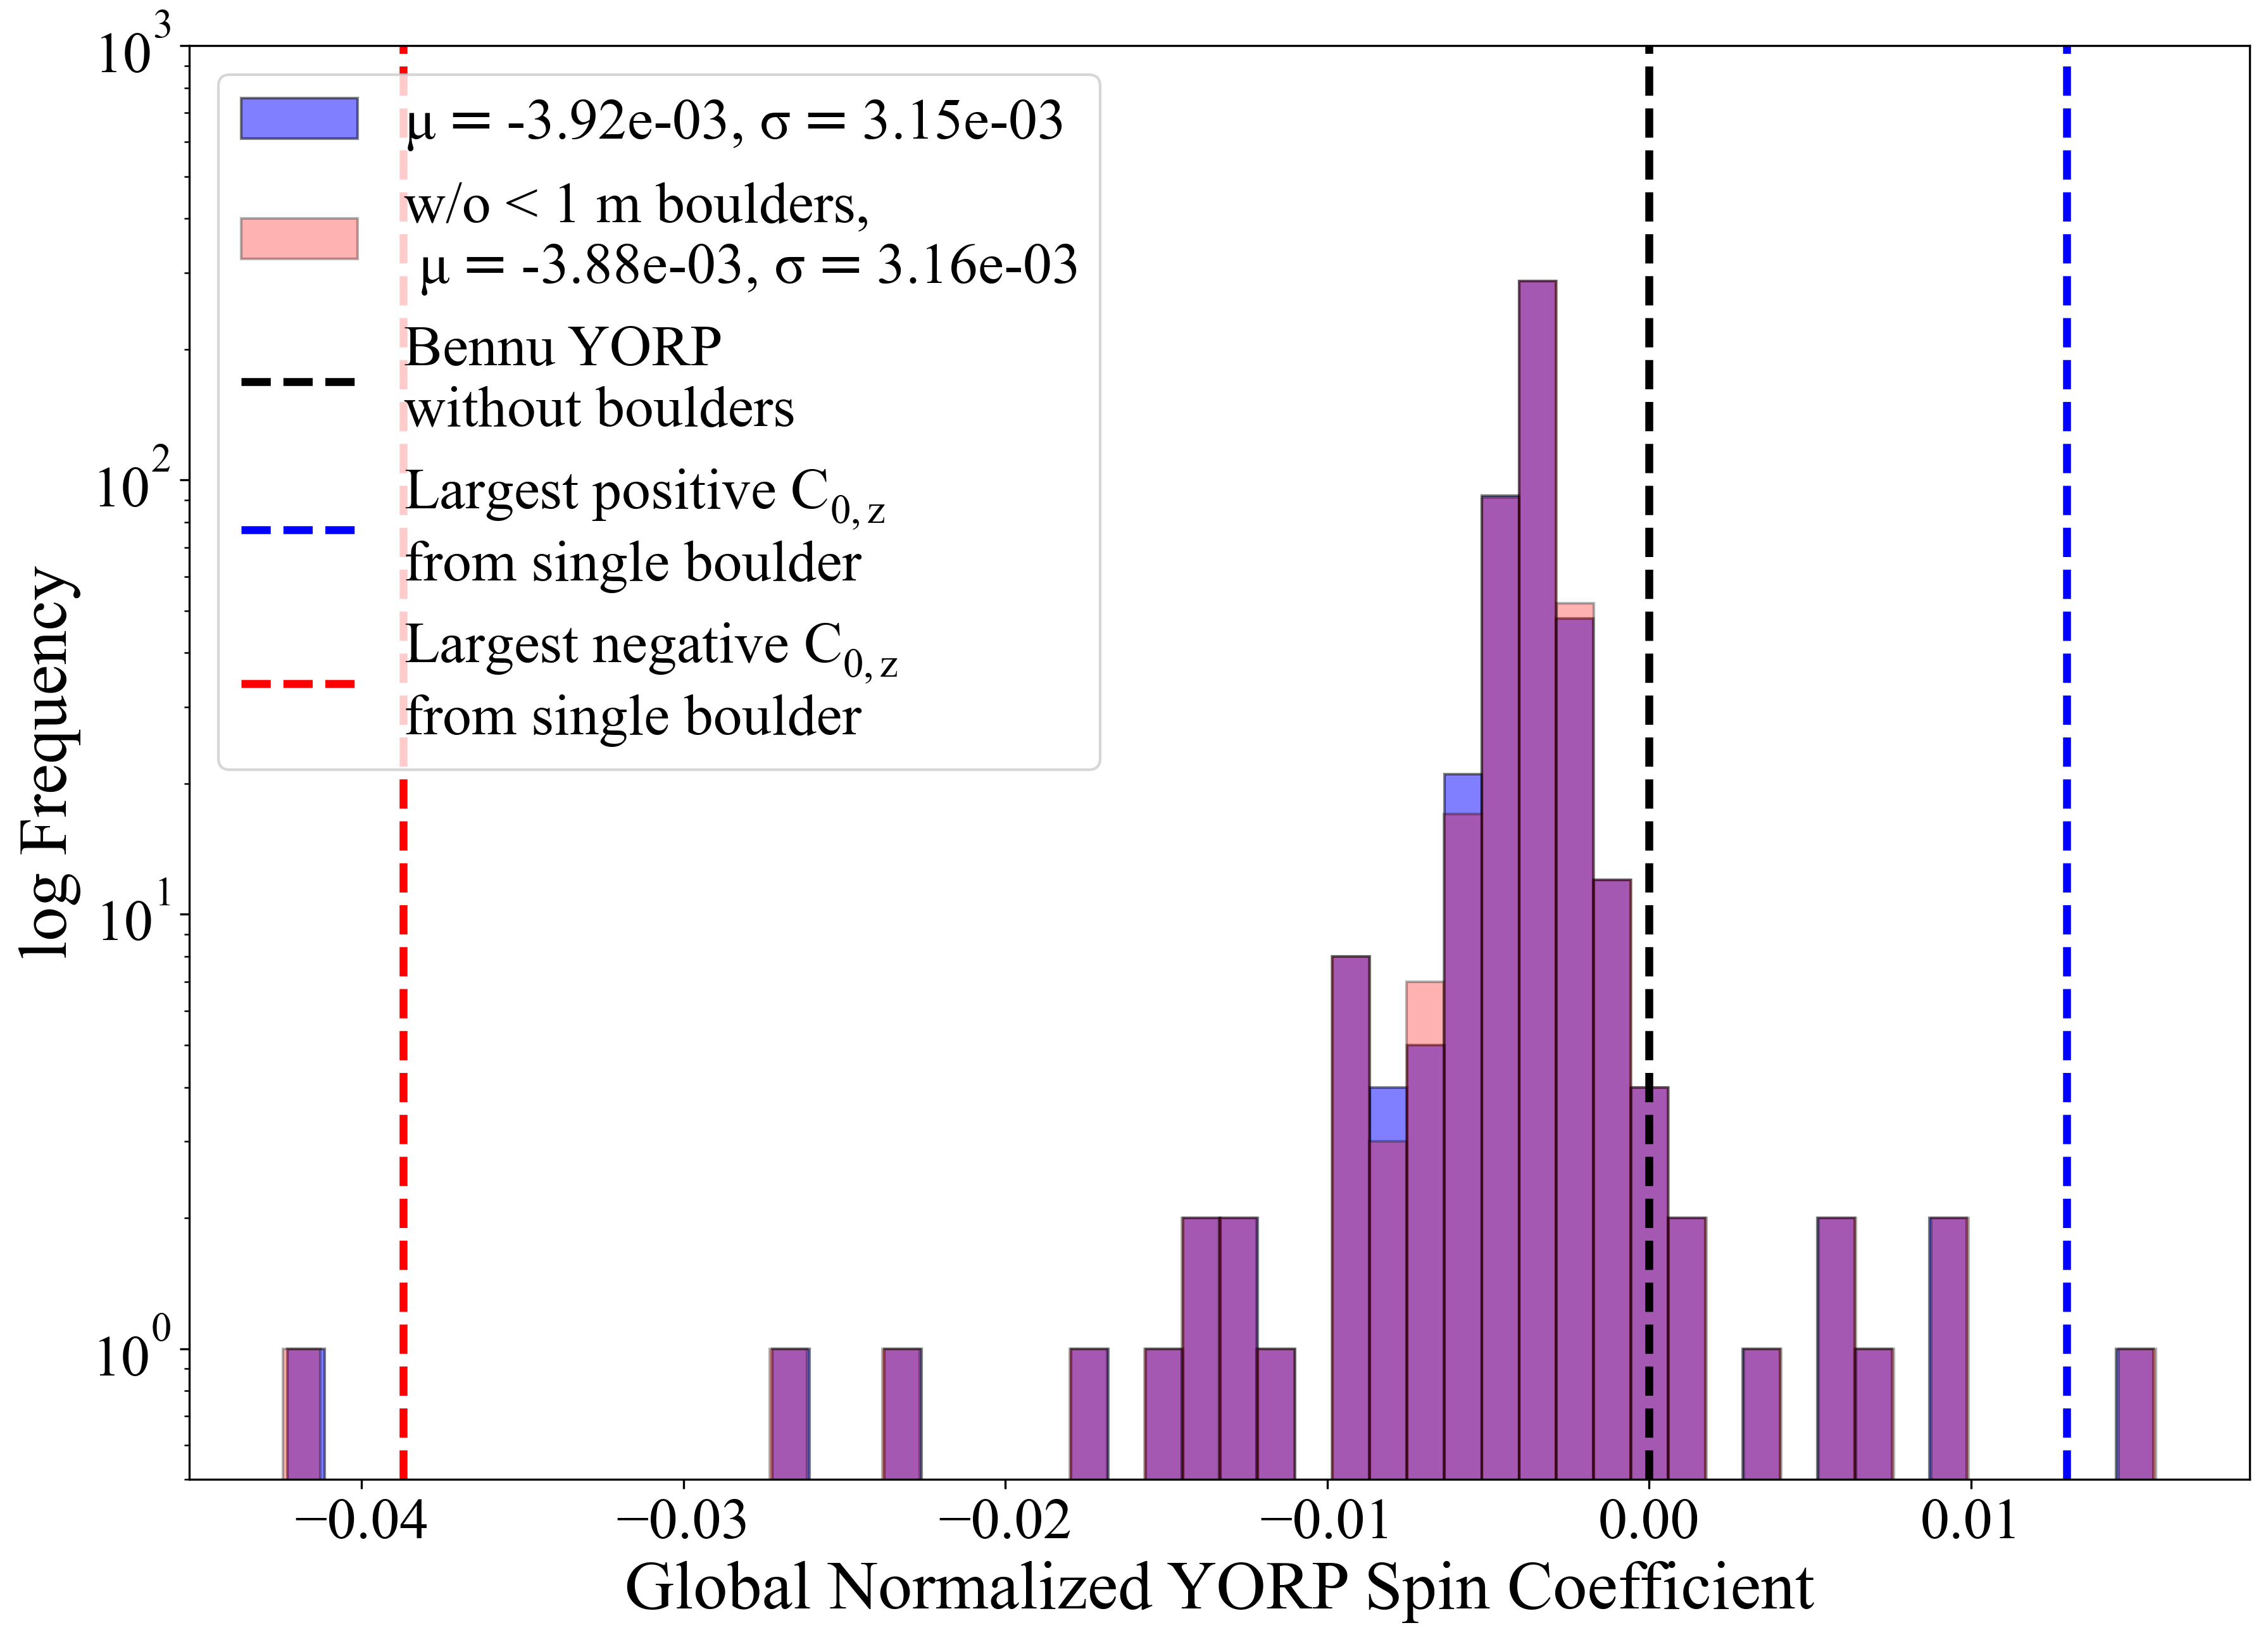
\includegraphics[width=0.45\textwidth]{fig/itokawa_comparison.png}
    \caption{Frequency distribution of total boulder YORP spin coefficients for Itokawa}
    \label{fig:itokawa_all_cases}
\end{figure}

\subsection{Large Influence Boulder Parameters}
\subsubsection{Size Comparison}
Itokawa has a population of boulders similar to Bennu in this simulation, 10 cm to 50 m and a size power law coefficient of 3.05. In Fig.\ref{fig:ito_percents} is the distribution of boulders that impact Itokawa's YORP spin with more than a 1\% contribution, compared by spin coefficient. The difference in mean size between the resampled data and the filtered impactful data is 16 times larger than the population mean, compared to the 500\% seen for Bennu. The number of boulders that provide more than 1\% of magnitude compared to the global YORP is 29.3\% of the 500 possible sets of 5000 boulders simulated. Note again that we are comparing magnitudes and not signs when considering this data, in order to illustrate the strength of YORP imparted by a single feature in the positive or negative direction. As was discussed in Sec. \ref{analysis}, the sign of YORP is evenly distributed as the orientation changes and therefore a dampening of this effect is seen when considering a large number of boulders in a population. 
\begin{figure}[H]
    \centering
    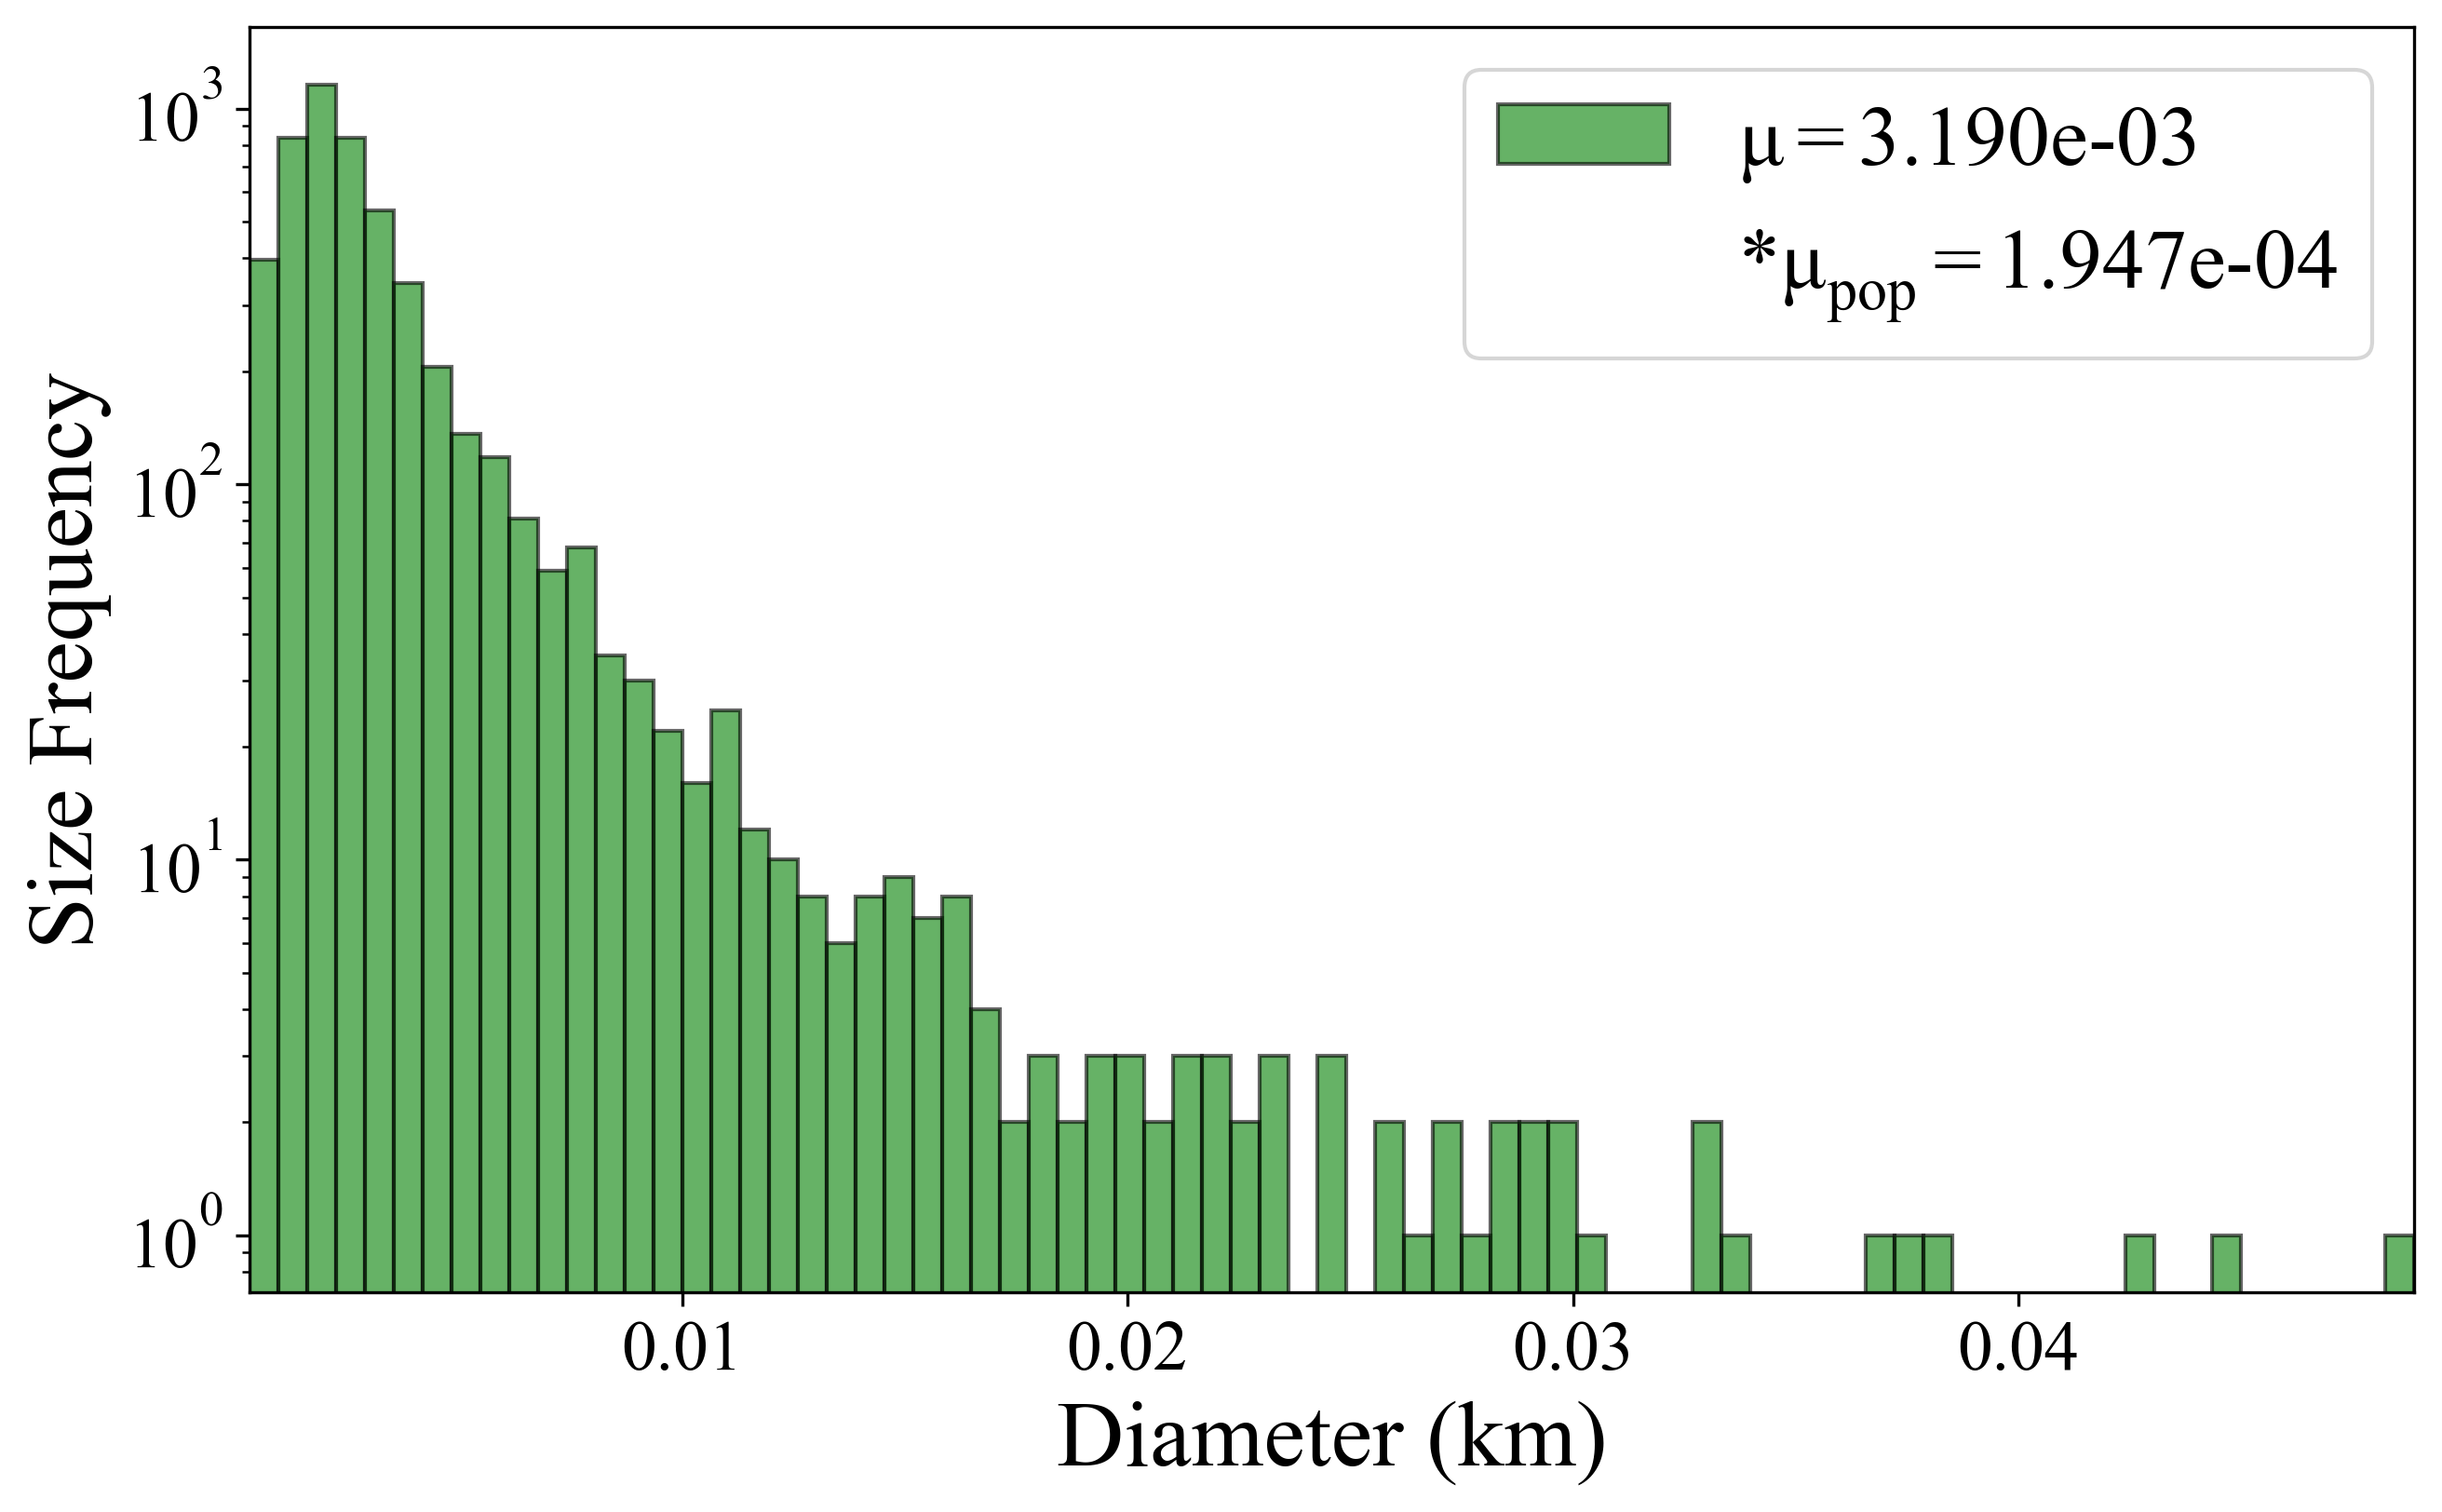
\includegraphics[width=0.42\textwidth]{fig/itokawa_impact_size_new.png}
    \caption{Size distribution and mean diameter of boulders where $C_{0,z,i} > 1\%$ for Itokawa}
    \label{fig:ito_percents}
\end{figure}
\begin{figure*}[t]
    \centering
    \begin{subfigure}[t]{0.48\textwidth}
        \centering
        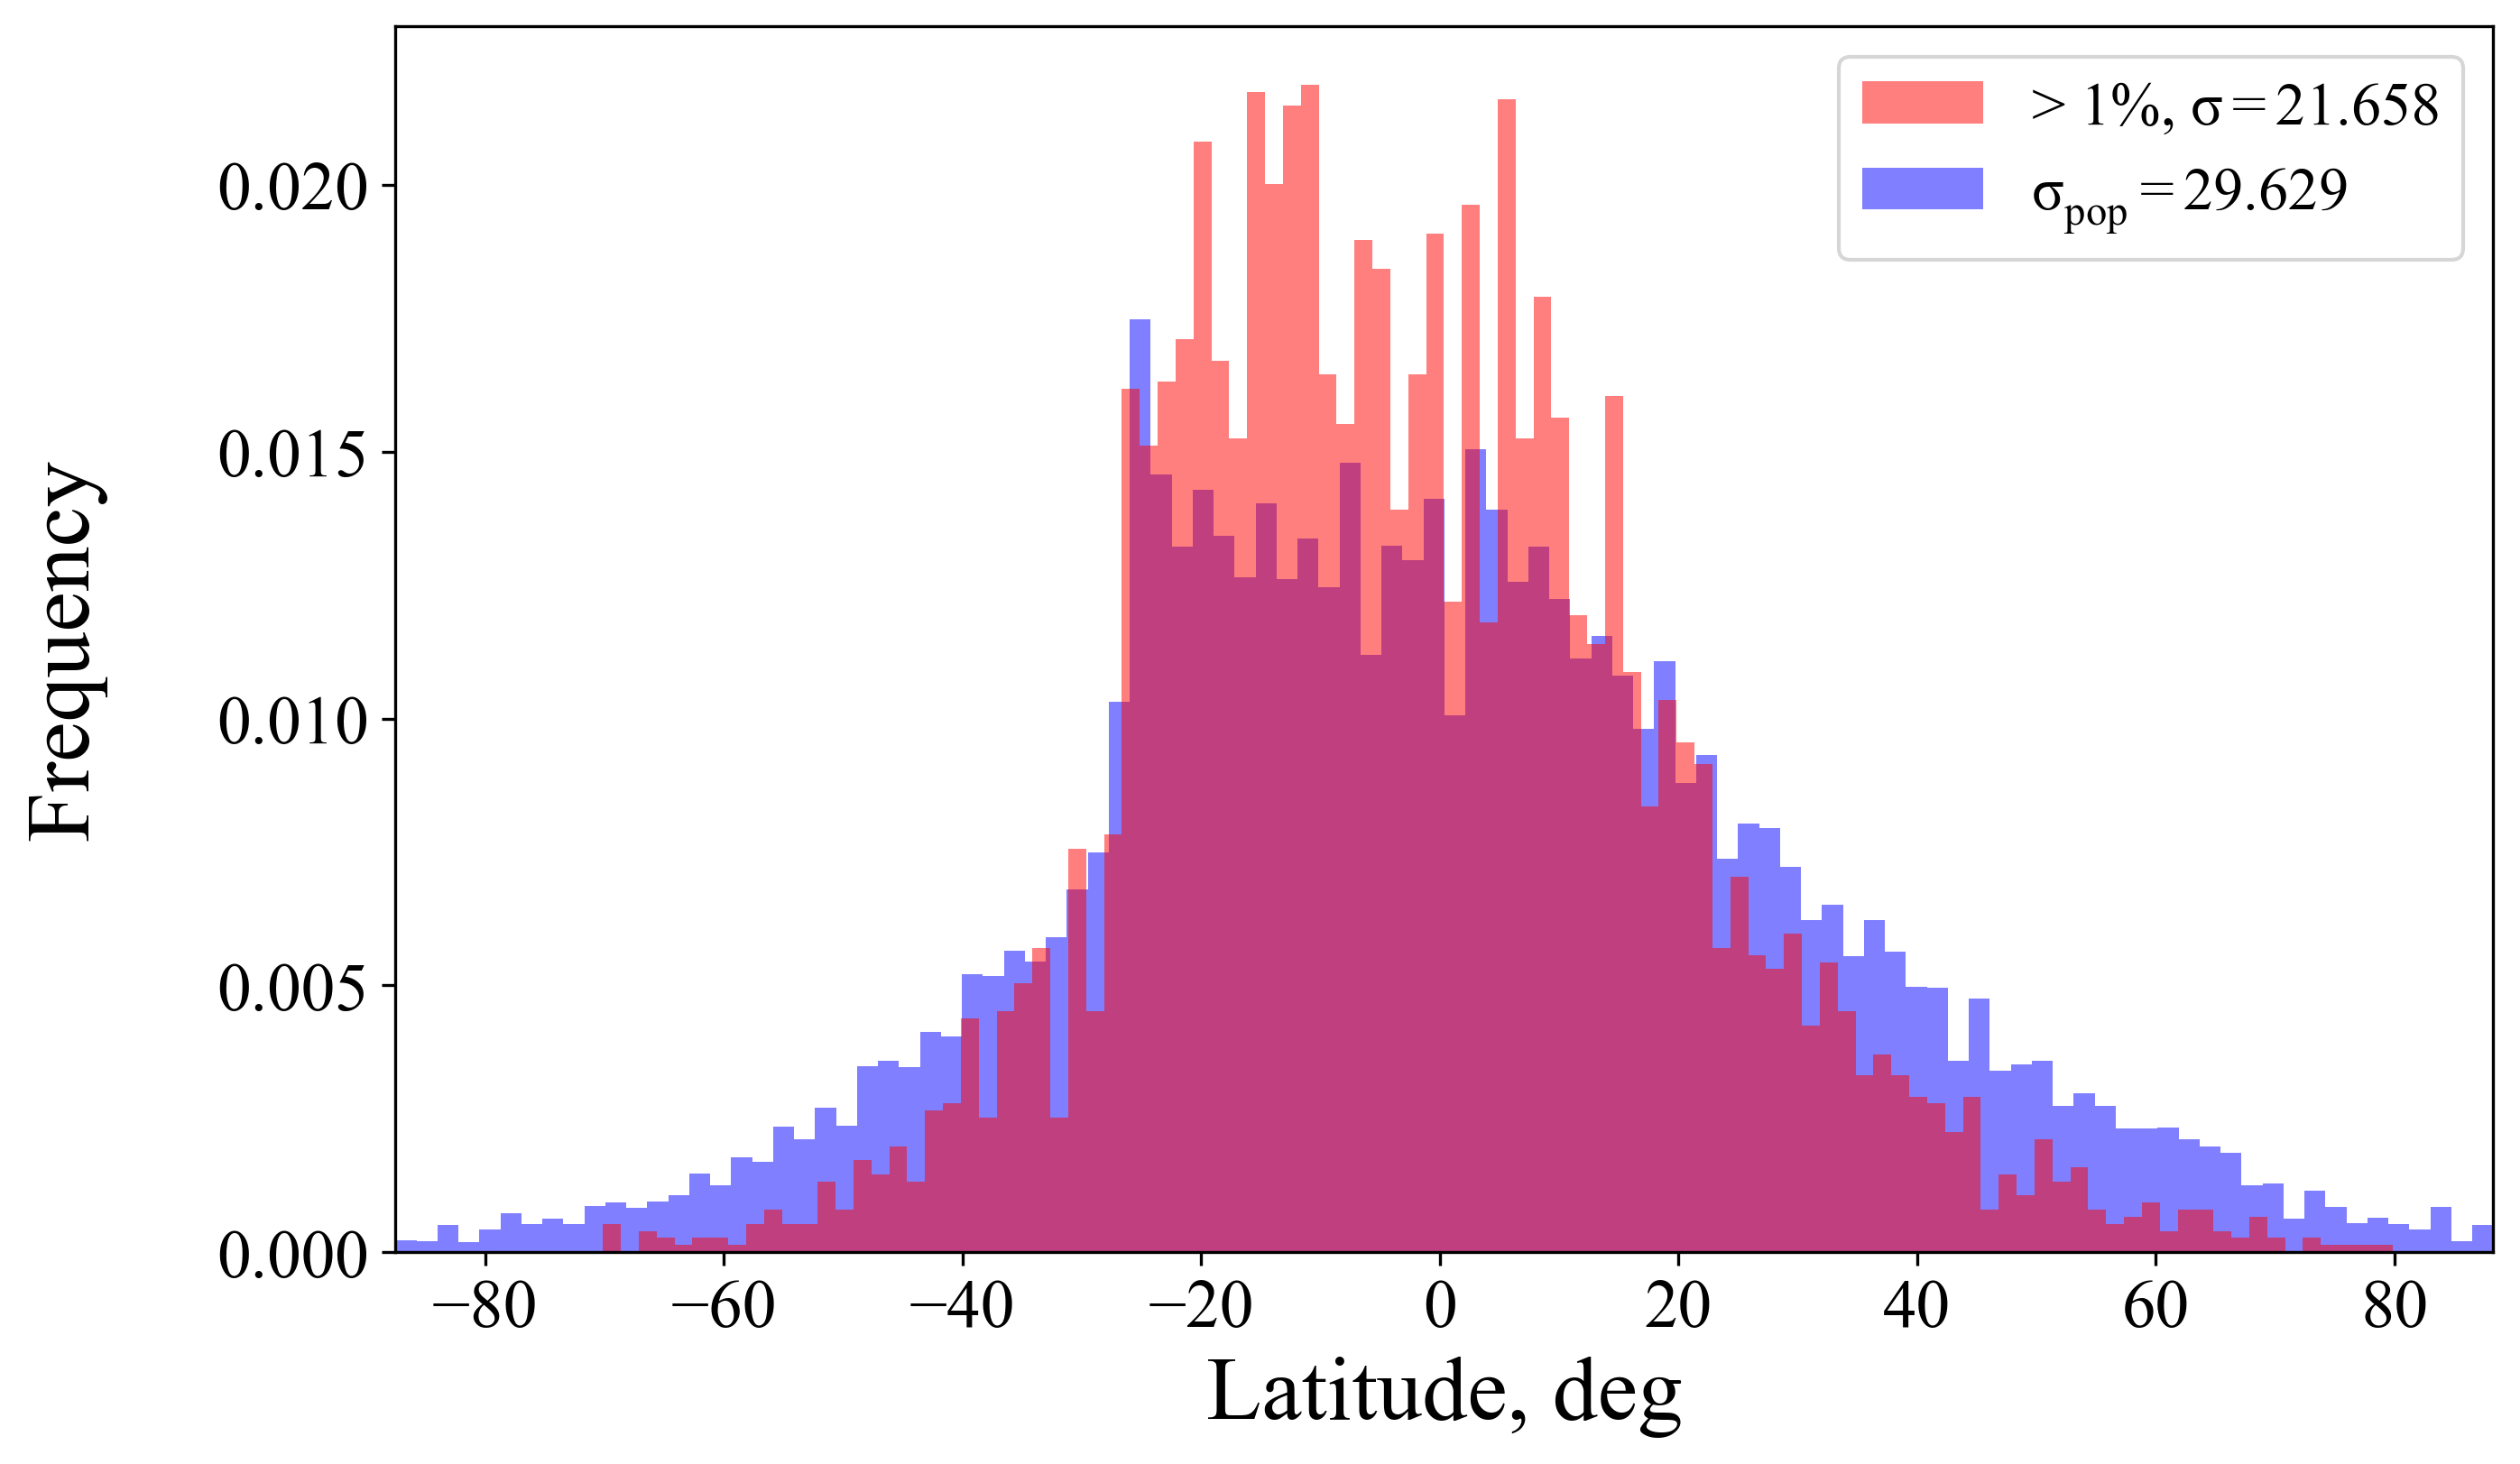
\includegraphics[width=\textwidth]{fig/itokawa_impact_location_new.png}
        \caption{Latitude distribution of impactful boulders and the entire population set on Itokawa}
        \label{fig:ito_latitudes}
    \end{subfigure}
    \hfill
    \begin{subfigure}[t]{0.49\textwidth}
        \centering
        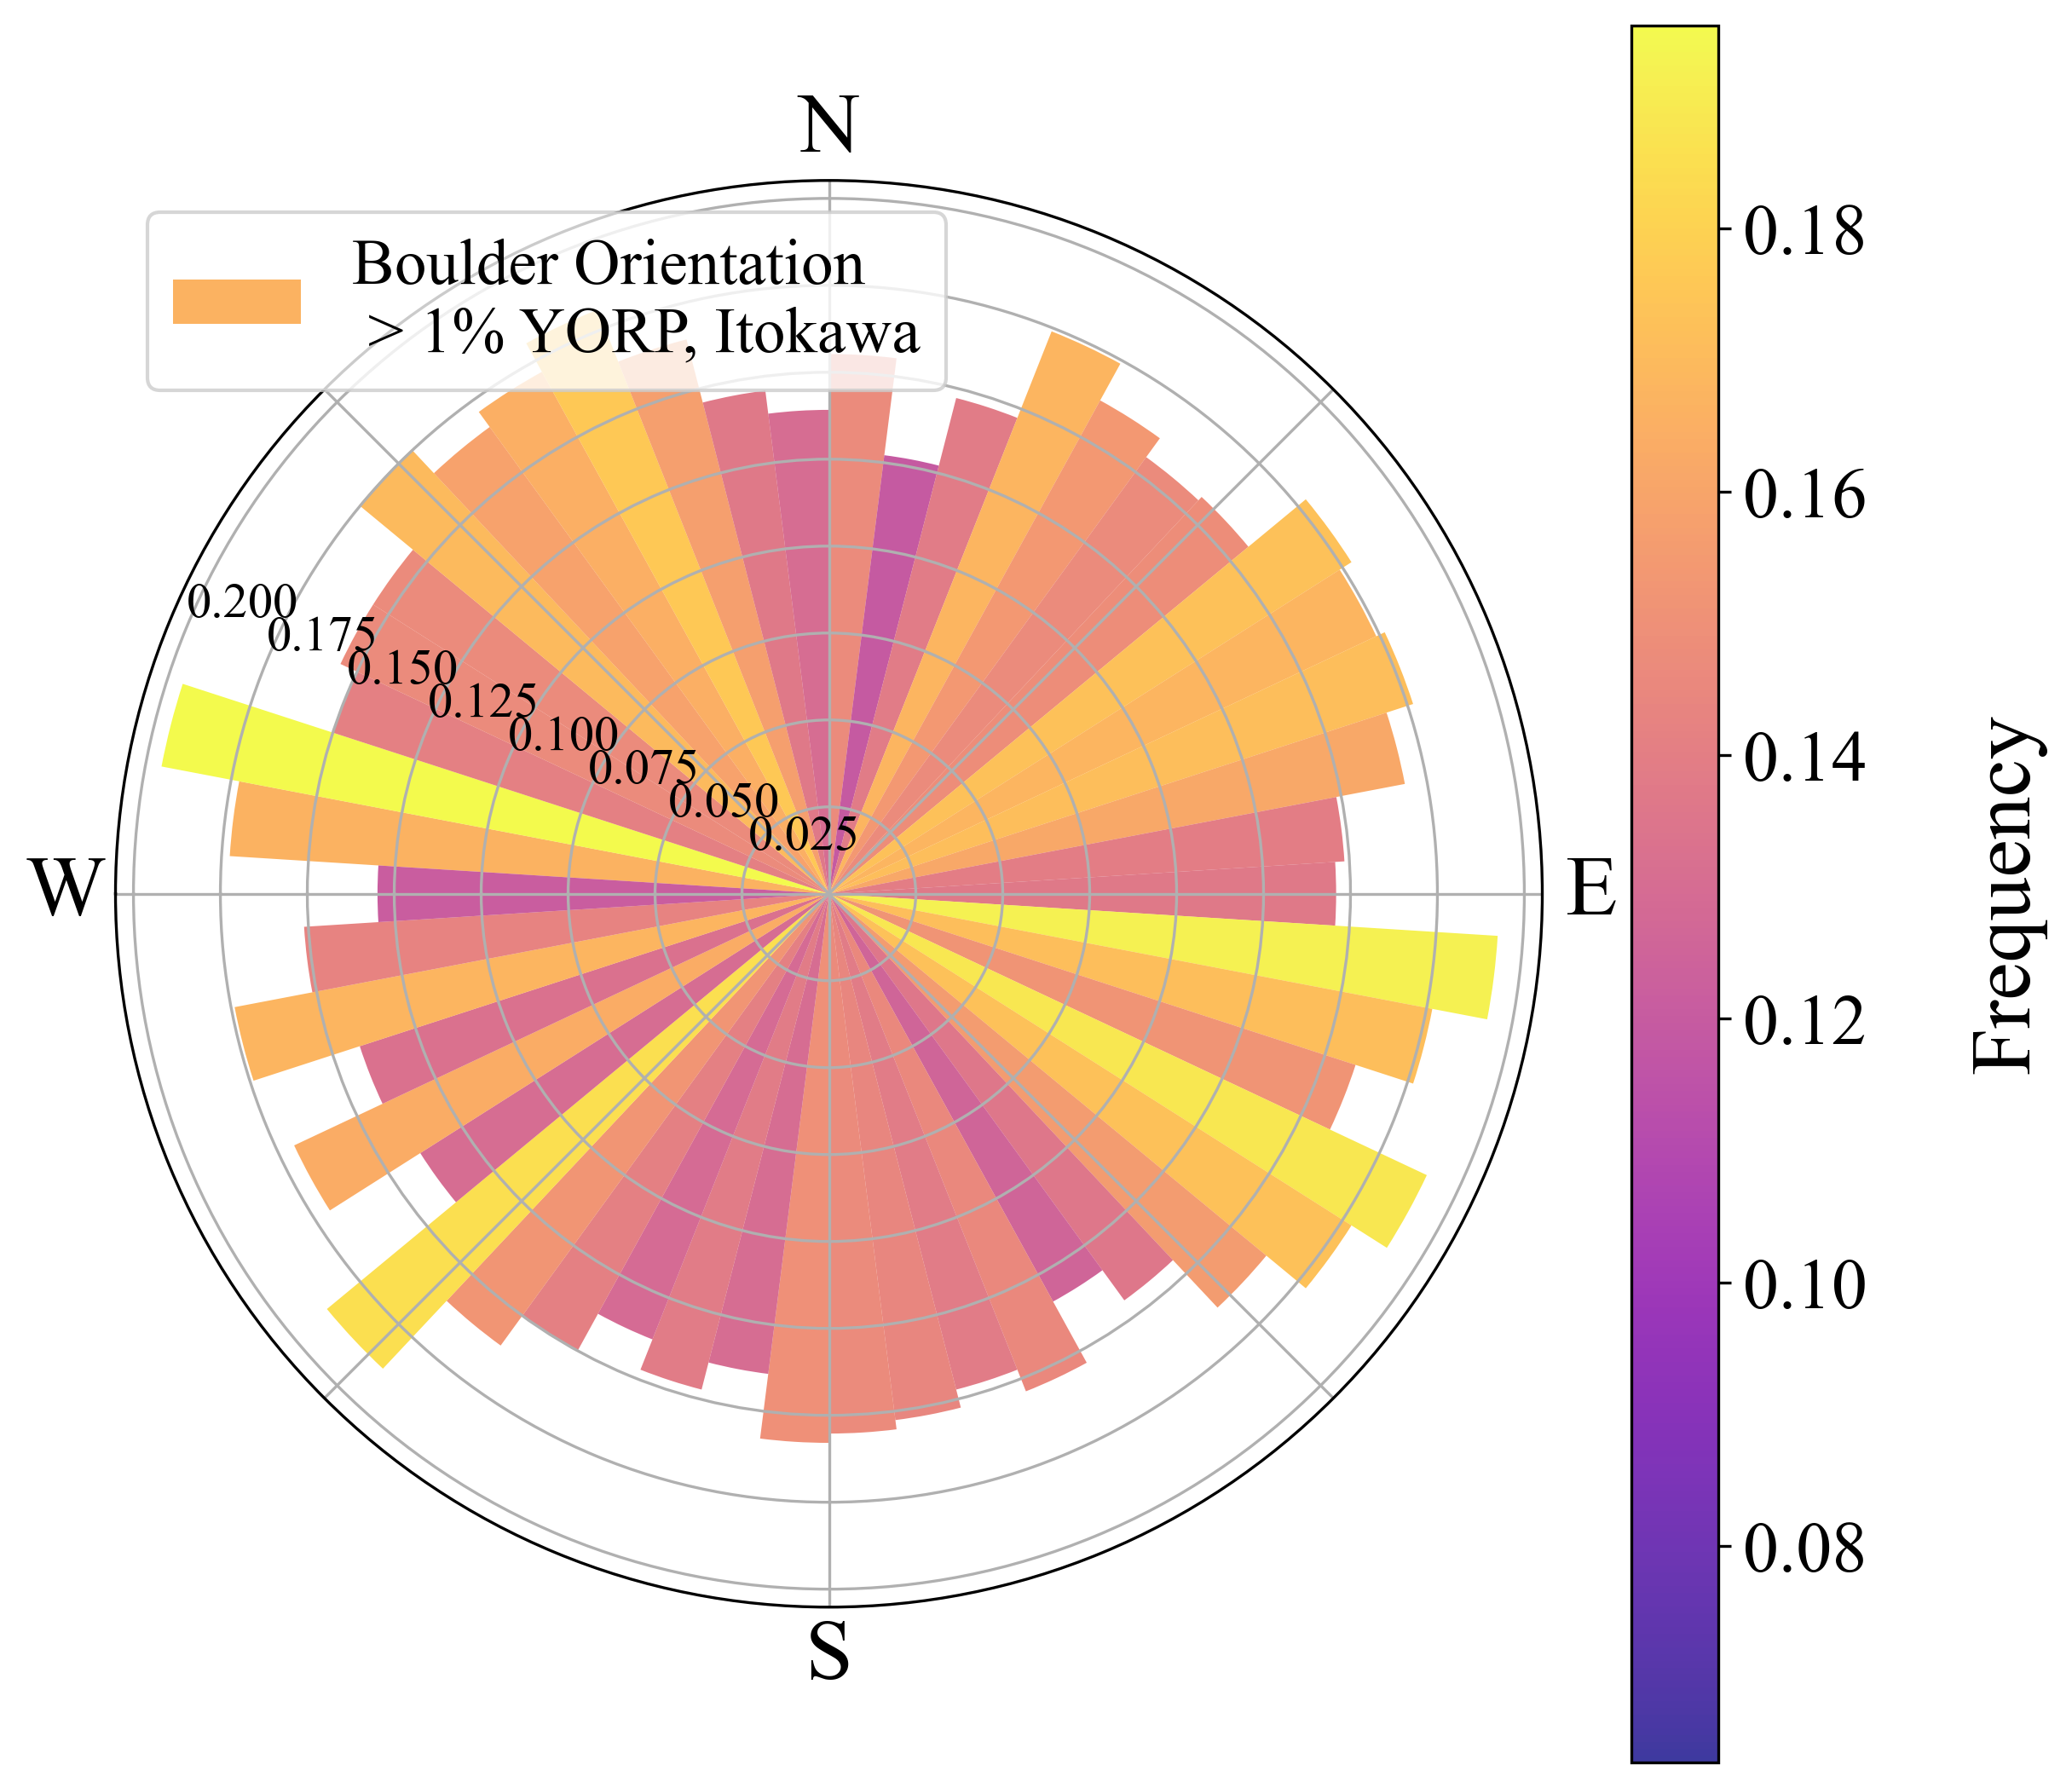
\includegraphics[width=0.75\textwidth]{fig/itokawa_impact_orient_new.png}
        \caption{Frequency of boulder orientation for the impactful boulder population on Itokawa}
        \label{fig:ito_orientation}
    \end{subfigure}
    \caption{Itokawa distribution comparison of normalized frequencies of boulder latitude and orientation in the > 1\% YORP spin coefficient boulder population.}
    \label{fig:itokawa_results}
\end{figure*}
\subsubsection{Location: Sub-30 Degree Latitude Preference}

We see in Fig.\ref{fig:itokawa_results}a, there is a natural tendency for boulders with longer lever arms, such as ones found at the far lengths along the equator, to have a larger YORP spin coefficient. The standard deviation of the latitude distribution of boulders that contribute more than 1\% to global YORP is 27\% smaller than the full population. This is a more dramatic relationship than seen in the Bennu influential latitude distribution. The frequency of boulder latitude between $\pm30^{\circ}$ on Itokawa is at times double the population distribution frequency. Itokawa has longer torque arms at the equator relative to non-equatorial latitudes and this feature is pronounced in the ellipsoid versus a spheroidal shape.


\subsubsection{Orientation Bias: No Pattern}
The impact of orientation changes on Itokawa have a much more dampened effect versus the spheroidal shape of Bennu. There is a larger collection of impactful boulders in the directly east direction, but at a much lower variation of 7\% difference from the full population of uniformly distributed boulders. It is a barely perceptible difference in the full distribution seen in Fig.\ref{fig:itokawa_results}. Boulders pointing east had a stronger bias than any pointing directly west, but overall the variation from a uniform distribution is small.

The largest factor for defining an impactful boulder in Itokawa is the torque arm, which in this shape is related to latitude. As seen in Fig. \ref{fig:heatmaps}, Itokawa has its largest positive and negative torque coefficients on the far regions of the head and posterior lobes. At these locations, a slight tilt in either the westerly or easterly directions can be magnified and therefore smaller boulders here will have a larger contribution to global YORP. There is more investigation to be done on the relationship of YORP torque and surface evolution as we see bodies like Bennu that have reached a relatively axi-symmetric spherical stable shape and attitude, while bodies like the contact binary Itokawa could be evolving away from or towards a more symmetric shape as the lobes contribute to YORP spin-down. 


\section{Sensitivity Analysis}\label{sens_analysis}

We find that for each body, the effective size required to contribute just $1\%$ to the global YORP acceleration can be relatively small and only bounded by the minimum of the possible distribution. The contribution ratio is also altered by properties that can increase the stochasticisty of YORP emission and even alter the sign of torque. By producing many models of boulder populations, we have provided a significant sample size in order to address the variance in the YORP effect due to boulders. Now we will show how sensitive our global YORP torque calculations are to limited size bounds, enforced directionality, and simulated latitude restrictions. This is to find how influential each component can be for our simulation set of boulders. 

\subsection{Size Thresholding}
The natural size distribution of boulders on a surface follows a steep power law. This entails that smaller boulders are much, much more likely to be found on a surface versus larger boulders. This fact was not necessary to prove, as we used observations from several rubble-pile asteroids as a basis for sampling. In this analysis, we focus on Bennu's boulder population as representative for both cases to detail the impact ratio of each boulder size on the global YORP torque. Further analysis is performed to compare boulder sensitivity on both bodies for orientation and location biases. 

\begin{figure}
    \centering
    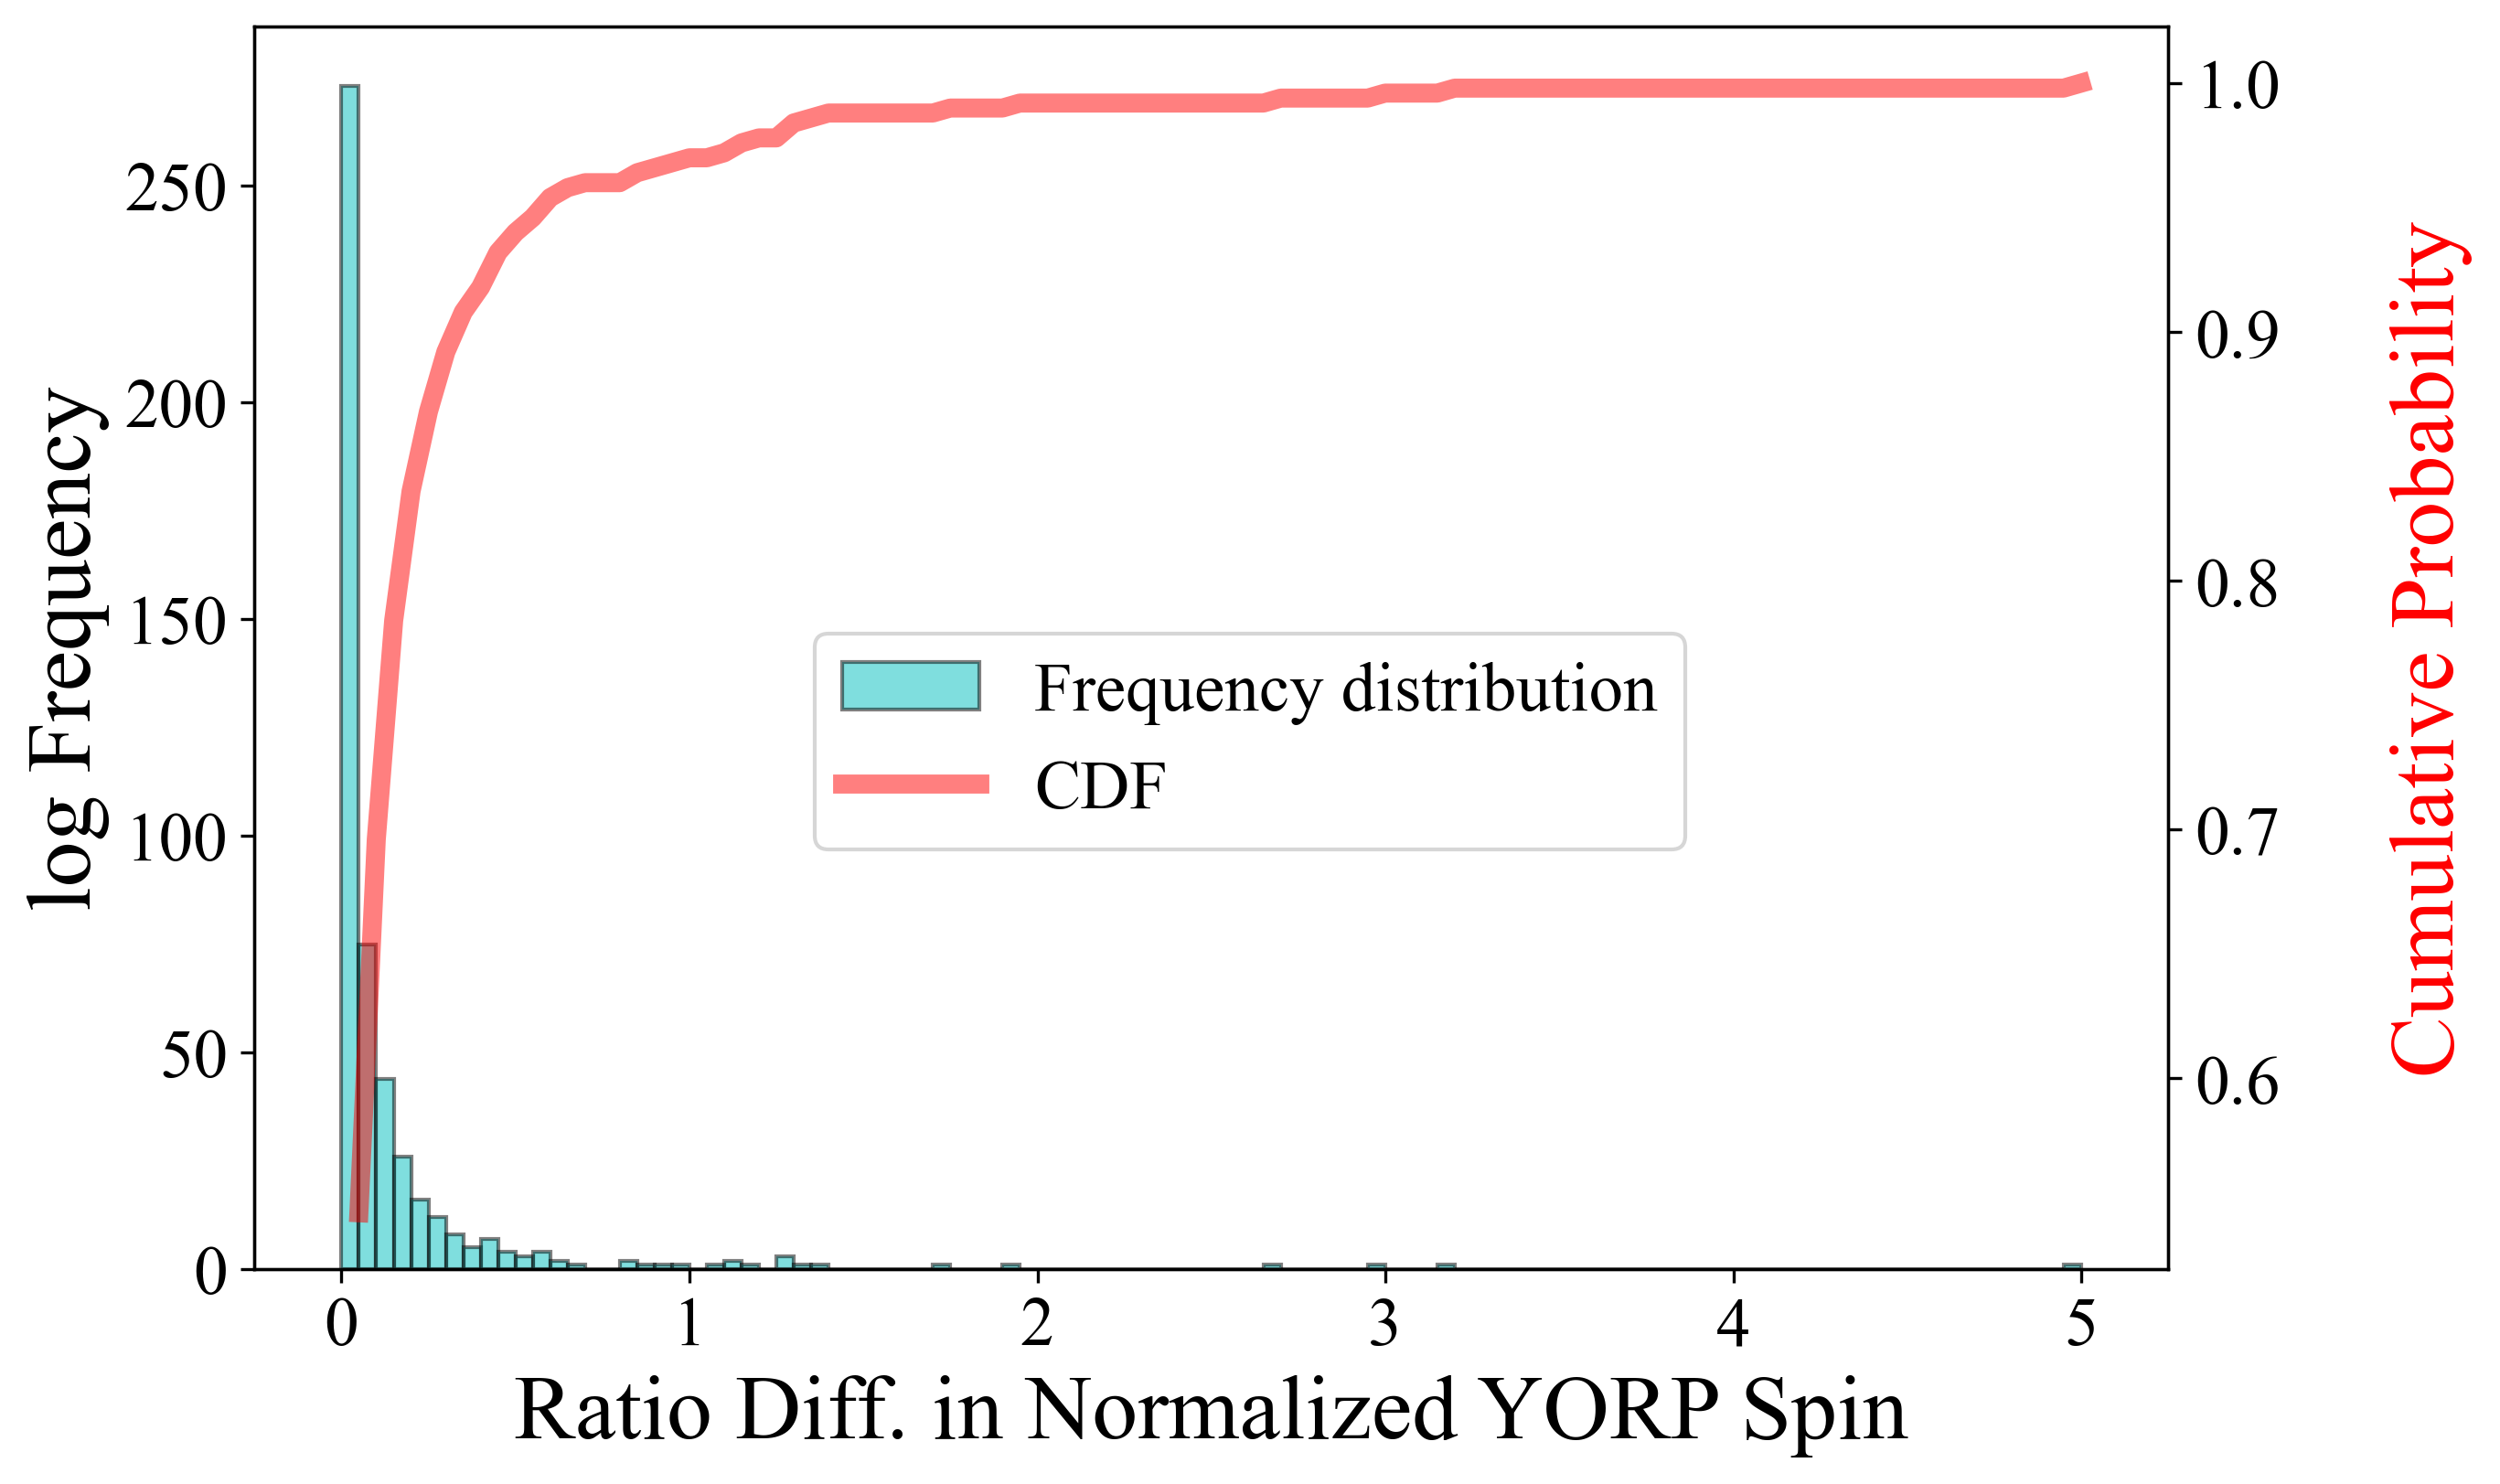
\includegraphics[width=0.45\textwidth]{fig/bennu_difference_yorps.png}
    \caption{Change in Bennu's global YORP spin coefficient with boulders, shown in Fig.\ref{fig:bennu_results}, when removing boulders < 1m, roughly $99\%$ of original population.}
    \label{fig:bennu_diff}
\end{figure}
When estimating YORP based on rough shapes, smaller boulders will not be observed or captured in the resolution of the model. In our simulation, the smallest boulder can be 10 cm in diameter, but in most studies, boulders around several meters are analyzed as they are easily observable and characterized. Here we compare the contribution of boulders by size range, binned in ranges of below 50 cm, between 50 cm and 1 m, between 1 m and 10 m, and above 10 m. This captures the size ranges that are both heavily sampled from our power law as well as the most obvious and impactful boulders on rubble-pile surfaces for bodies less than 1 km in diameter.
\begin{figure}[H]
    \centering
    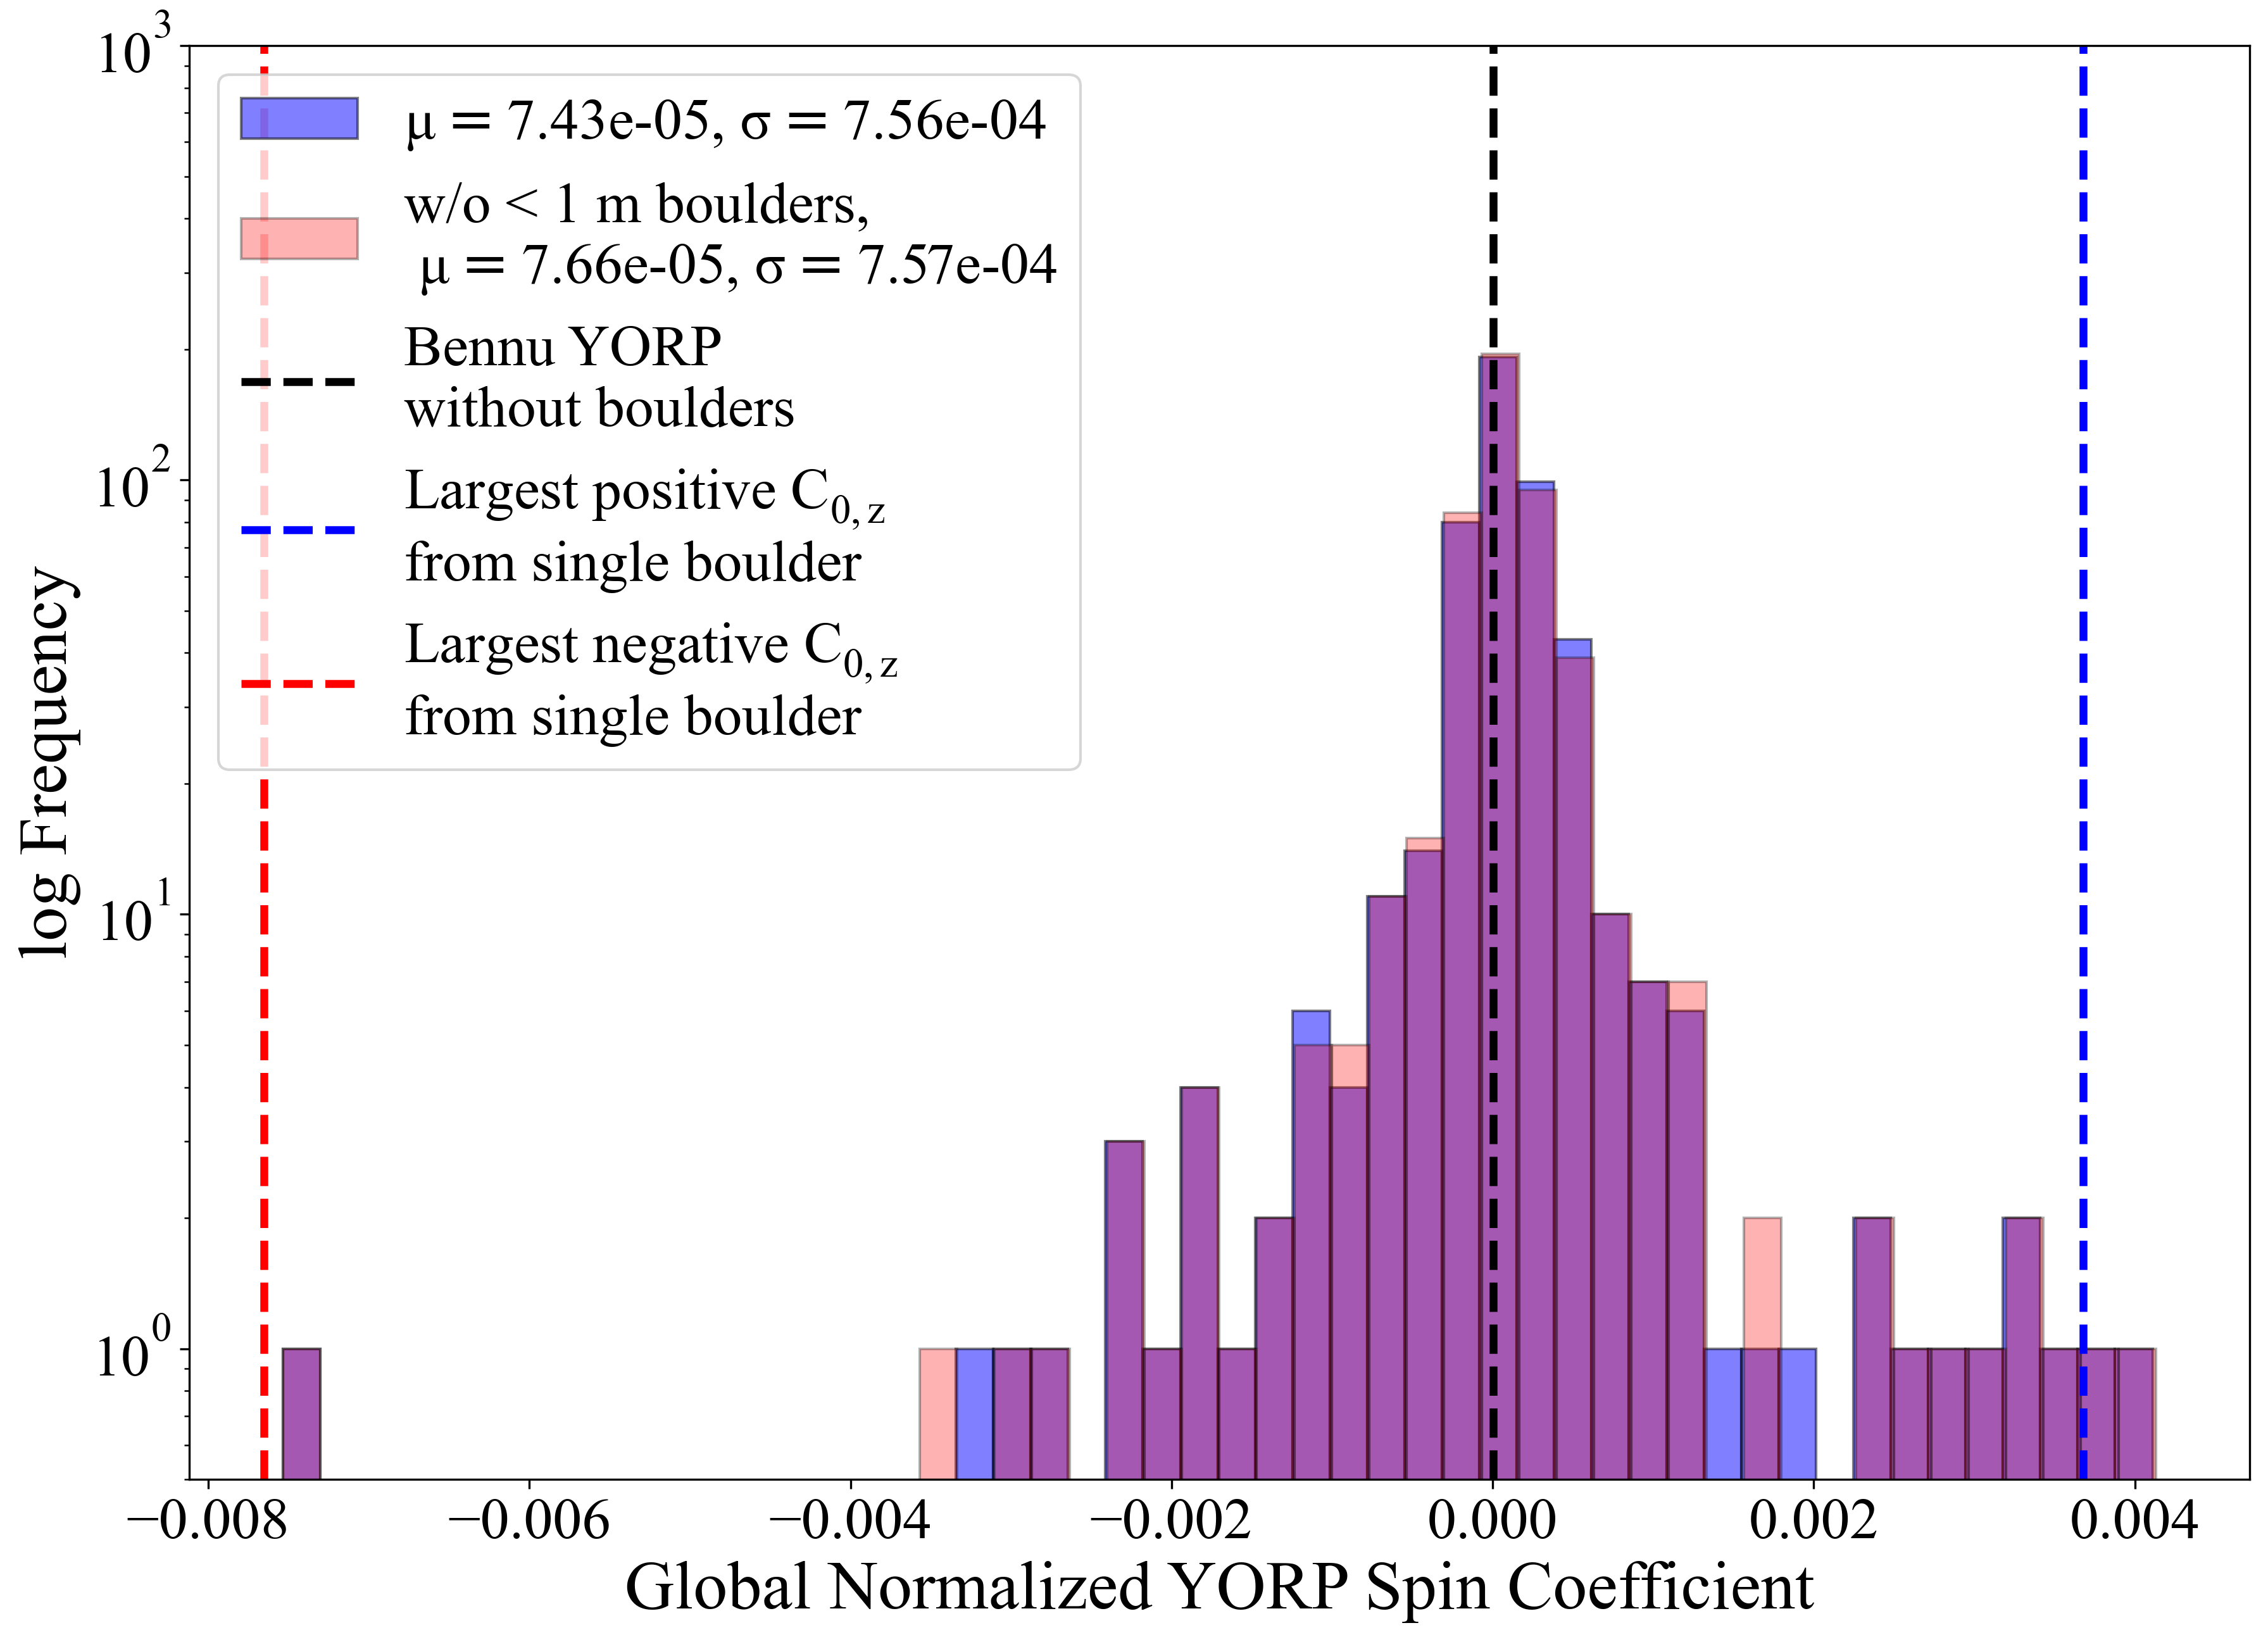
\includegraphics[width=0.42\textwidth]{fig/bennu_comparison_2.png}
    \caption{Overlaid distribution of normalized YORP with and without 1 m boulders}
    \label{fig:comparison}
\end{figure}
When the boulders less than 1 m in diameter are removed from the summation, we do not see a very large shift in the average global YORP. The distribution in Fig.\ref{fig:bennu_diff} shows a much higher frequency of changing YORP spin less than 50\% of the original value. This distribution is skewed by the large contributing boulders discussed in section \ref{bennu}. However, the cumulative distribution function shows an extremely steep increase below 100\% and continues to act asymptotically as we approach the single case where normalized YORP changes by 5 times the original value with the elimination of boulders less than 1m.

We capture the same population statistics when only $1.11\%$ of our original simulated features are considered, with the size bins and their associated YORP distributions given in Fig.\ref{fig:bins}. The result of filtering out boulders less than 1 m in diameter is shown in Fig. \ref{fig:comparison}. The mean of the distribution changes by 3\%. and standard deviation varies by 0.13\%. This is a powerful observation that can limit our further simulations to boulders of significant size and contributions instead of the full realistic size regime. This analysis is focusing on the variation in global YORP spin as it is totaled, versus the previous sections which looked at individual contributors by magnitude. We use a different metric for consideration of impact when considering the global YORP delta versus the individual boulder YORP.
\begin{figure}[H]
    \centering
    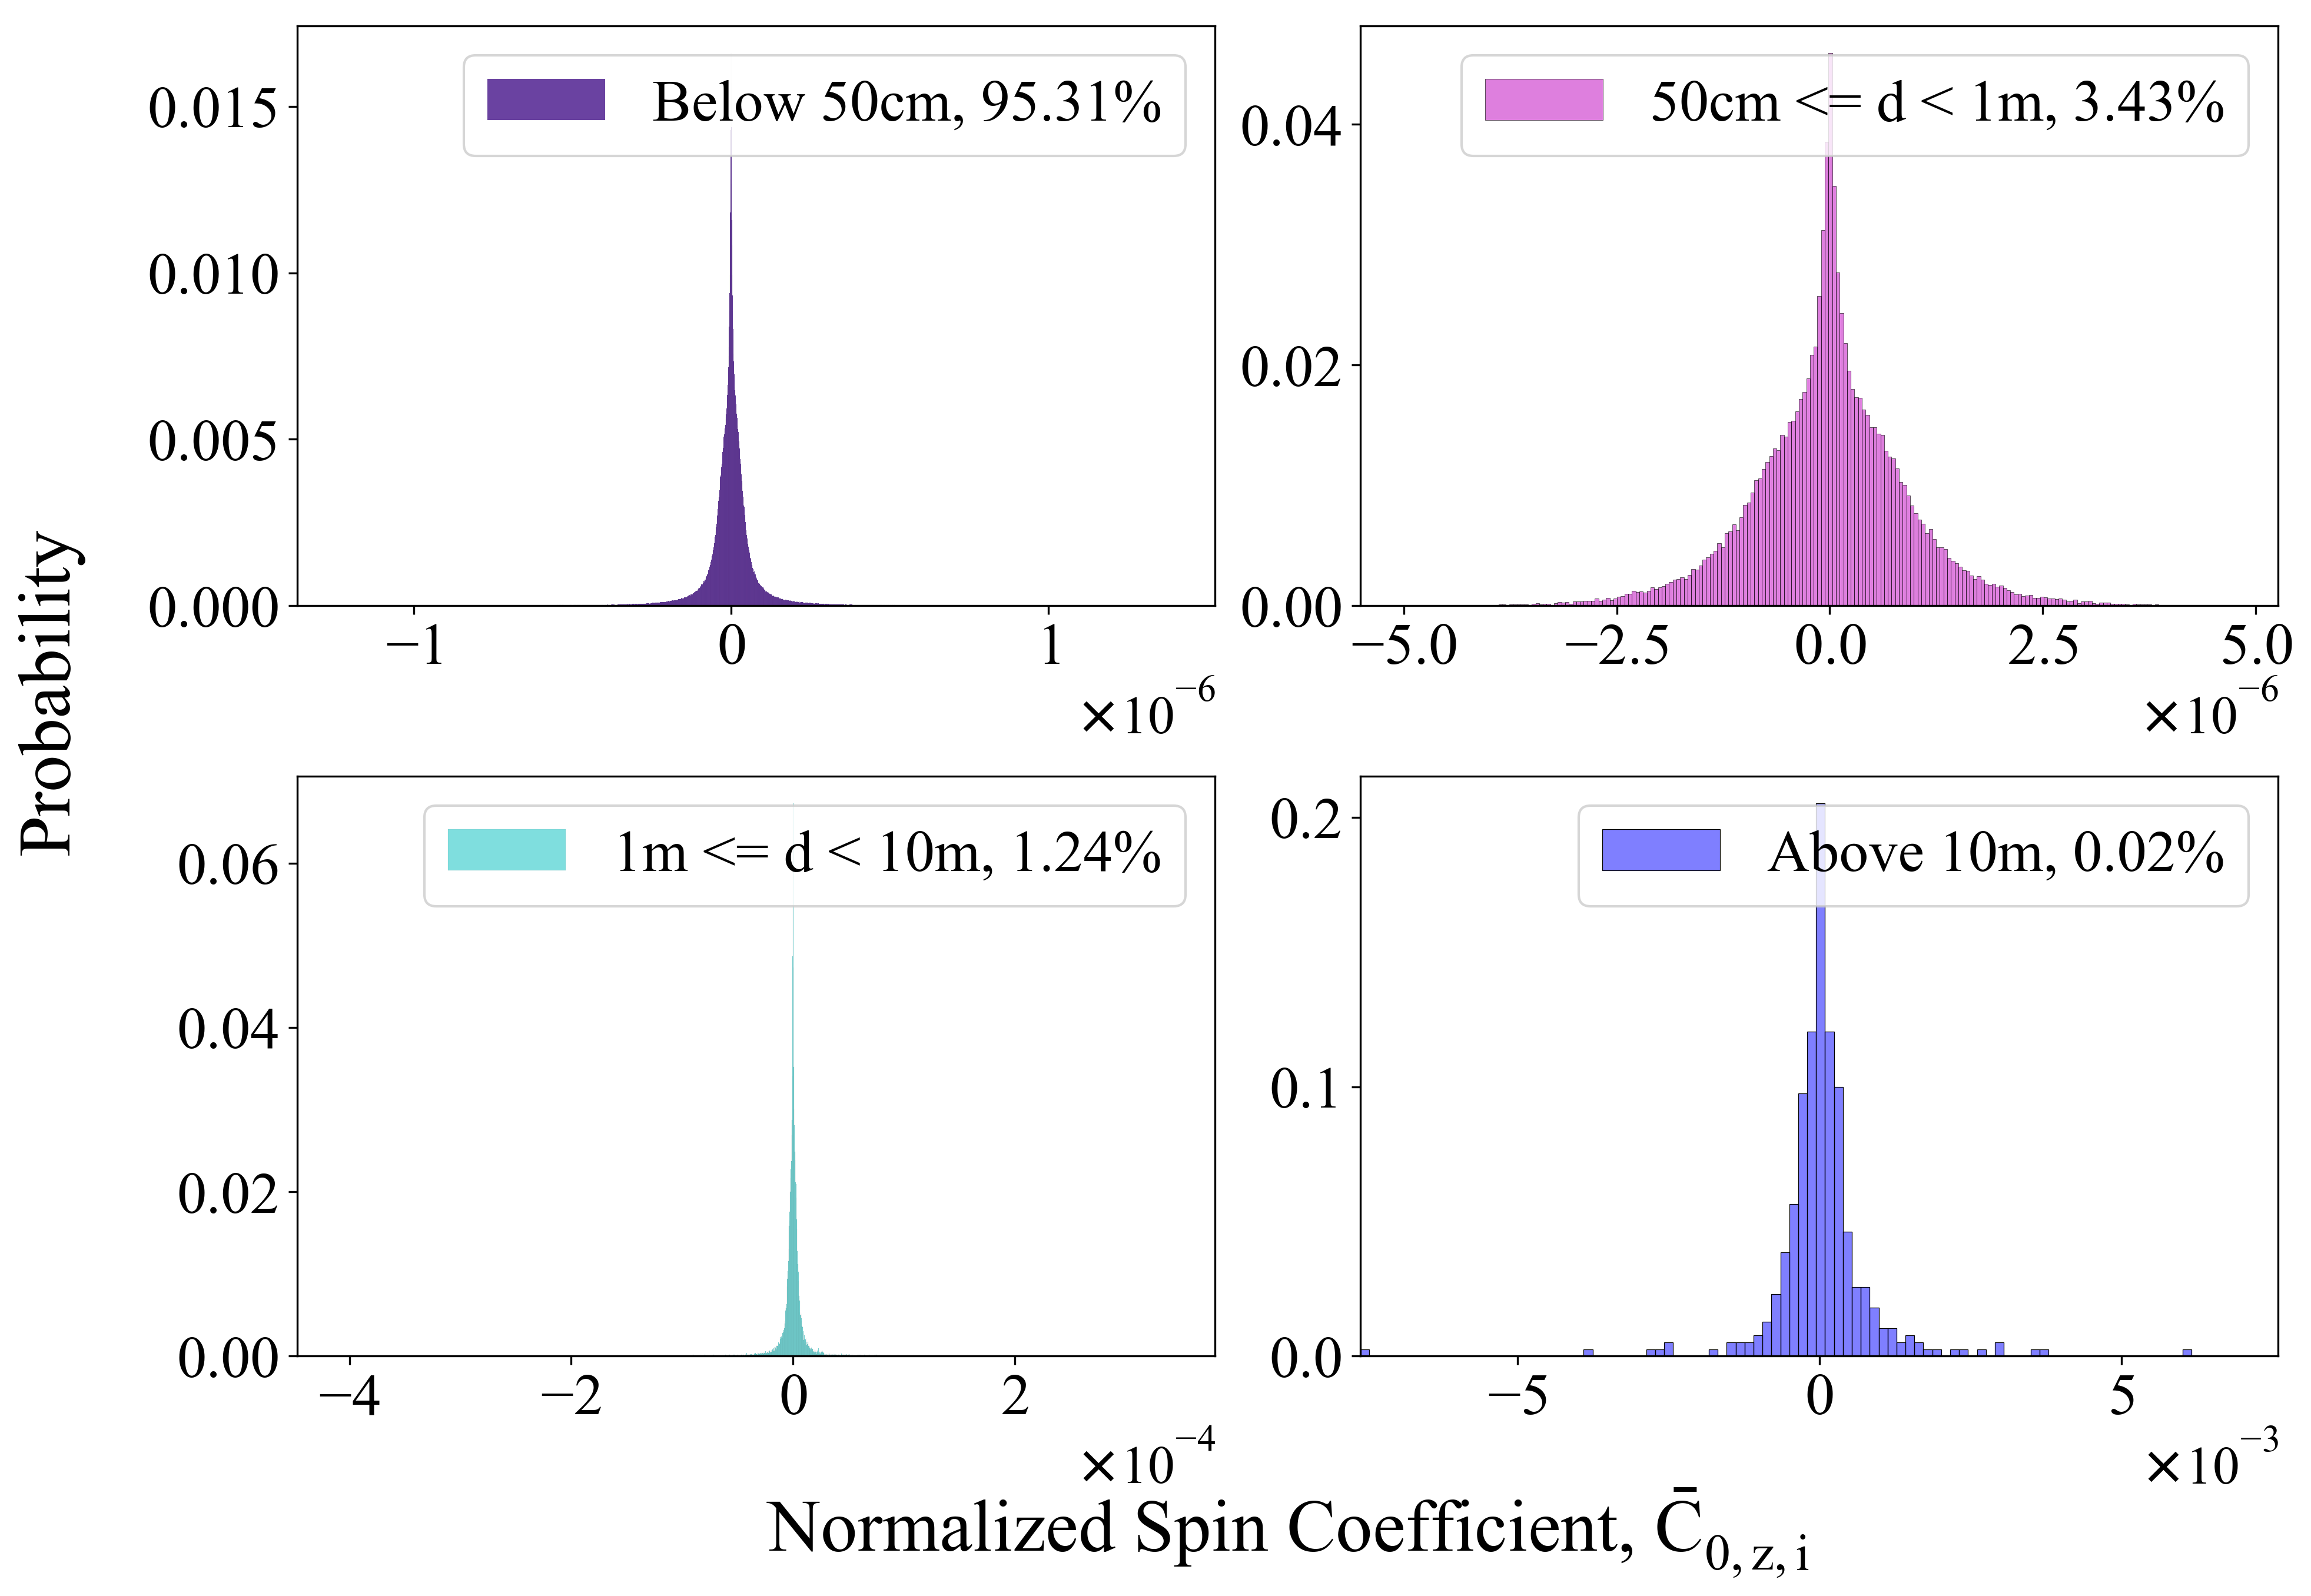
\includegraphics[width=0.49\textwidth]{fig/bennu_size_binned_spreads.png}
    \caption{Boulder spin coefficients for Bennu, separated by size bins. Percentages represent the proportion of boulders in each bin to the size of the sample population.}
    \label{fig:bins}
\end{figure}
There are large boulders seen on other asteroids that are possibly earlier on in their evolution. The boulder Dhol on the limb of the secondary of the Didymos system is estimated to be 16 m in diameter \cite{Daly2024} \cite{Pajola2024}. When compared to the 160 m diameter of the secondary itself, this is the same size fraction as the 54 m boulder seen on Bennu. Due to the deformation observed on Dimorphos, we expect that rubble-pile bodies with these mechanical properties will have young and dynamic surfaces \cite{Raducan2024}. Just one boulder of 10$\%$ of the overall body diameter can change YORP more than 100 times over or reverse its sign; however most of our simulated cases show a change in YORP of 10\% or less with the large population of mid-range boulders above 1 m making the bulk of the difference. As an asteroid evolves, it is less likely that the largest boulders will move and instead they may fragment and change their dominant orientation faces. We can also expect them to be buried if found at low latitudes or slope downhills, and conversely they may be excavated if found at high latitudes where material is flowing away from them. We discuss the implications of these circumstances in the coming sections.

\subsection{Orientation Biases: West Preference}
\begin{figure*}[t!]
    \centering
    \begin{subfigure}{0.49\textwidth}
        \centering
        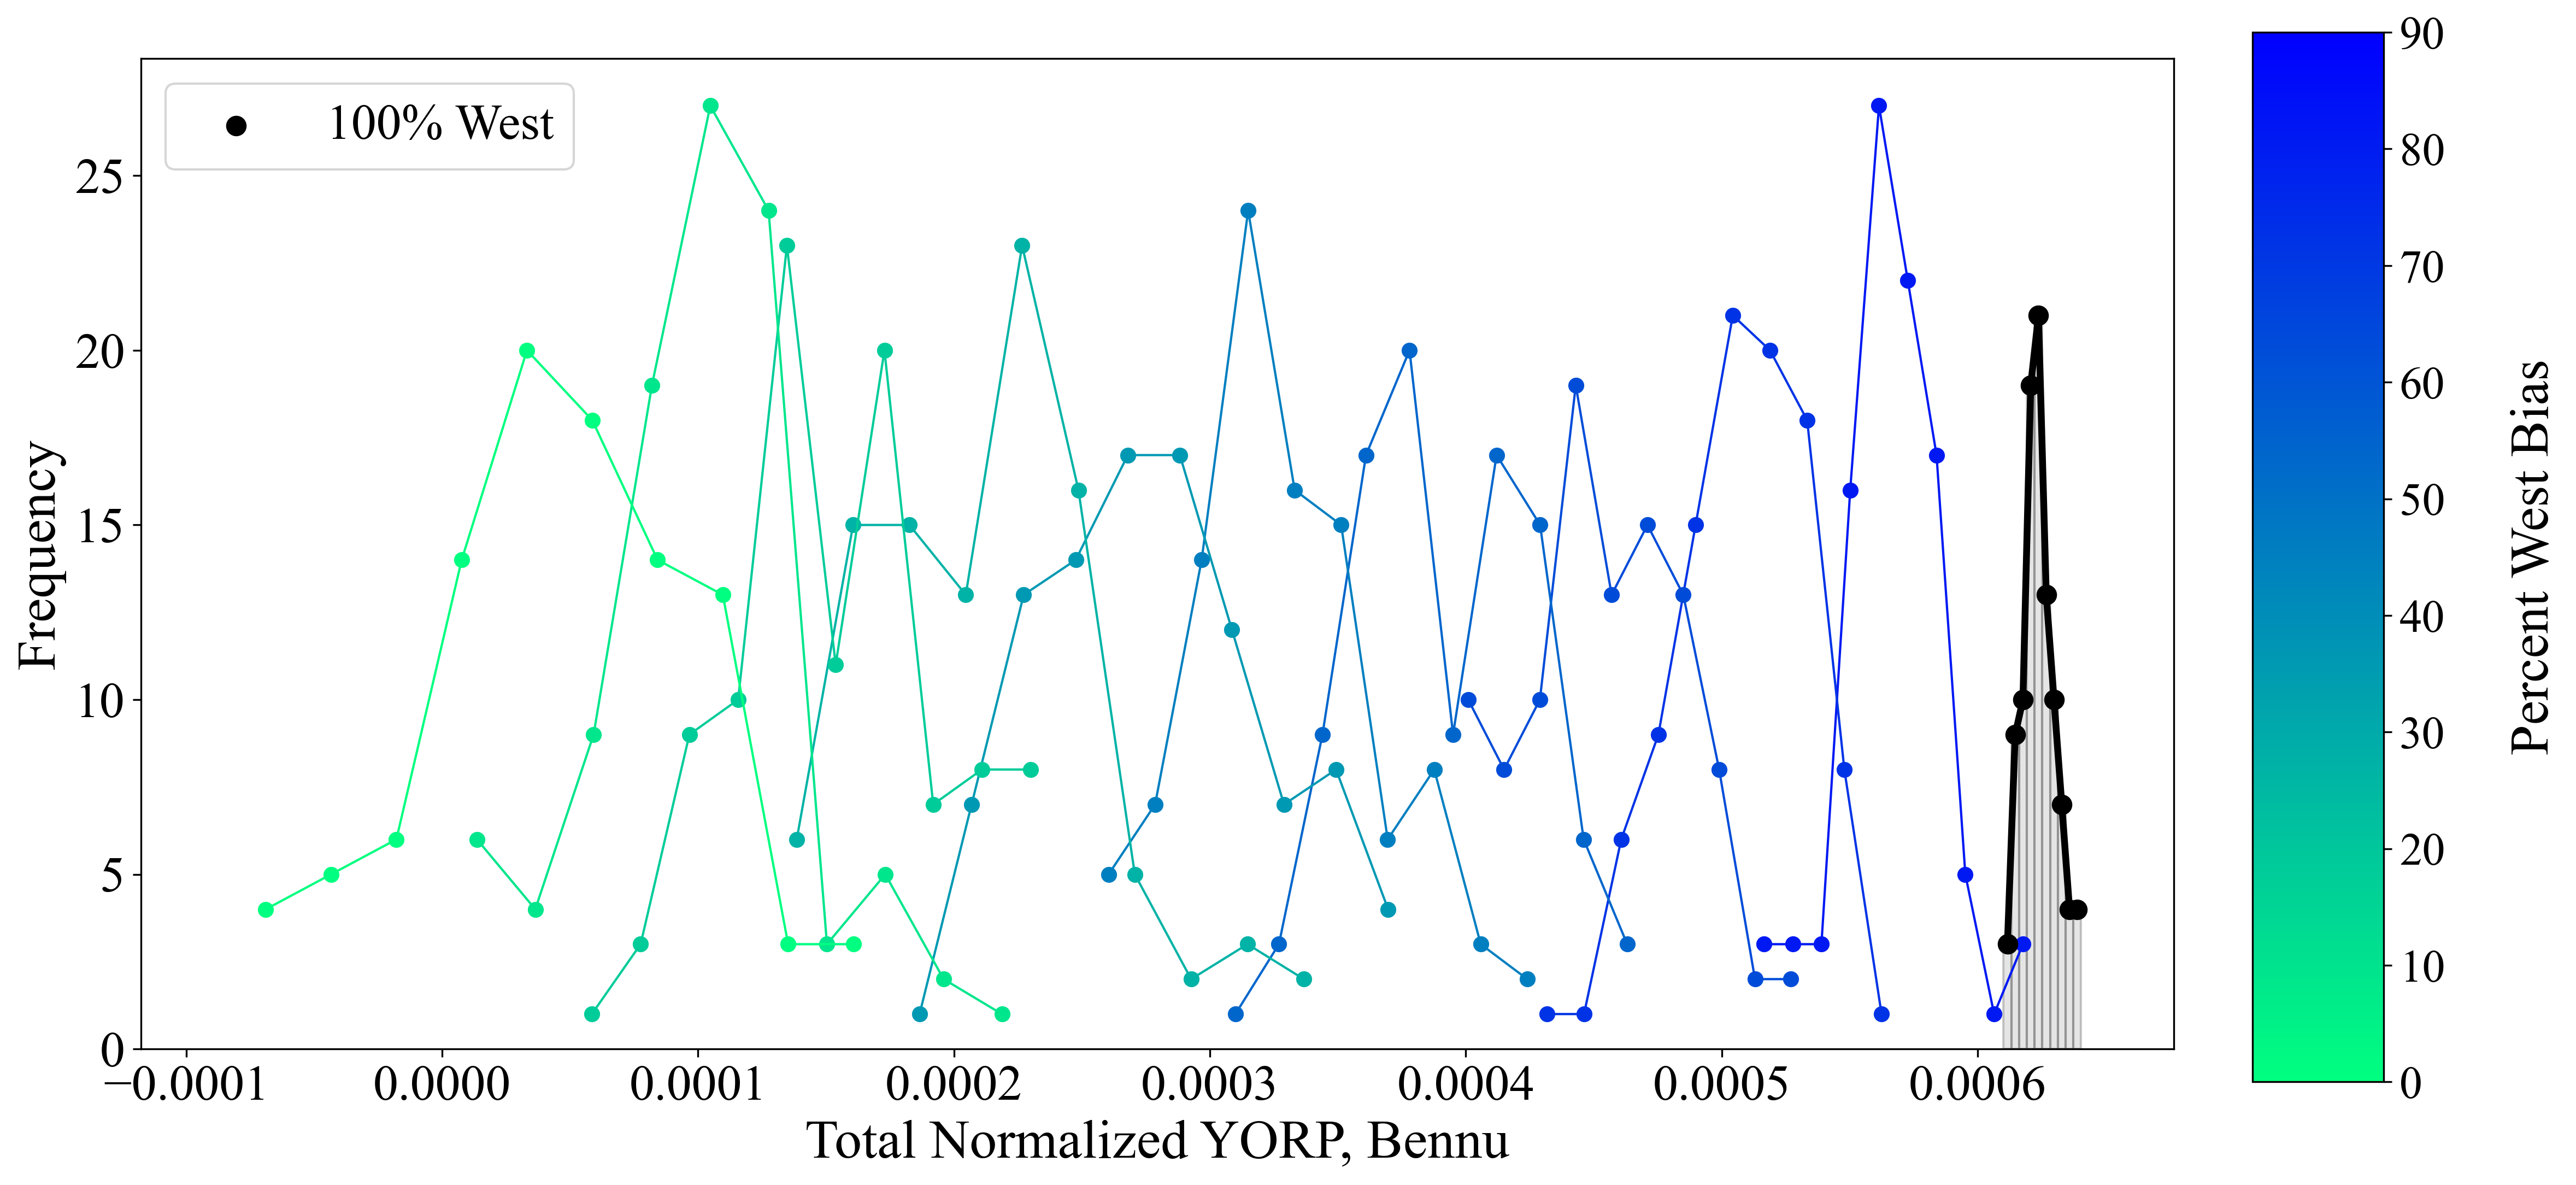
\includegraphics[width=\textwidth]{fig/bennu_orient_samesize_recreate.png}
    \end{subfigure}
    \hfill
    \begin{subfigure}{0.49\textwidth}
        \centering
        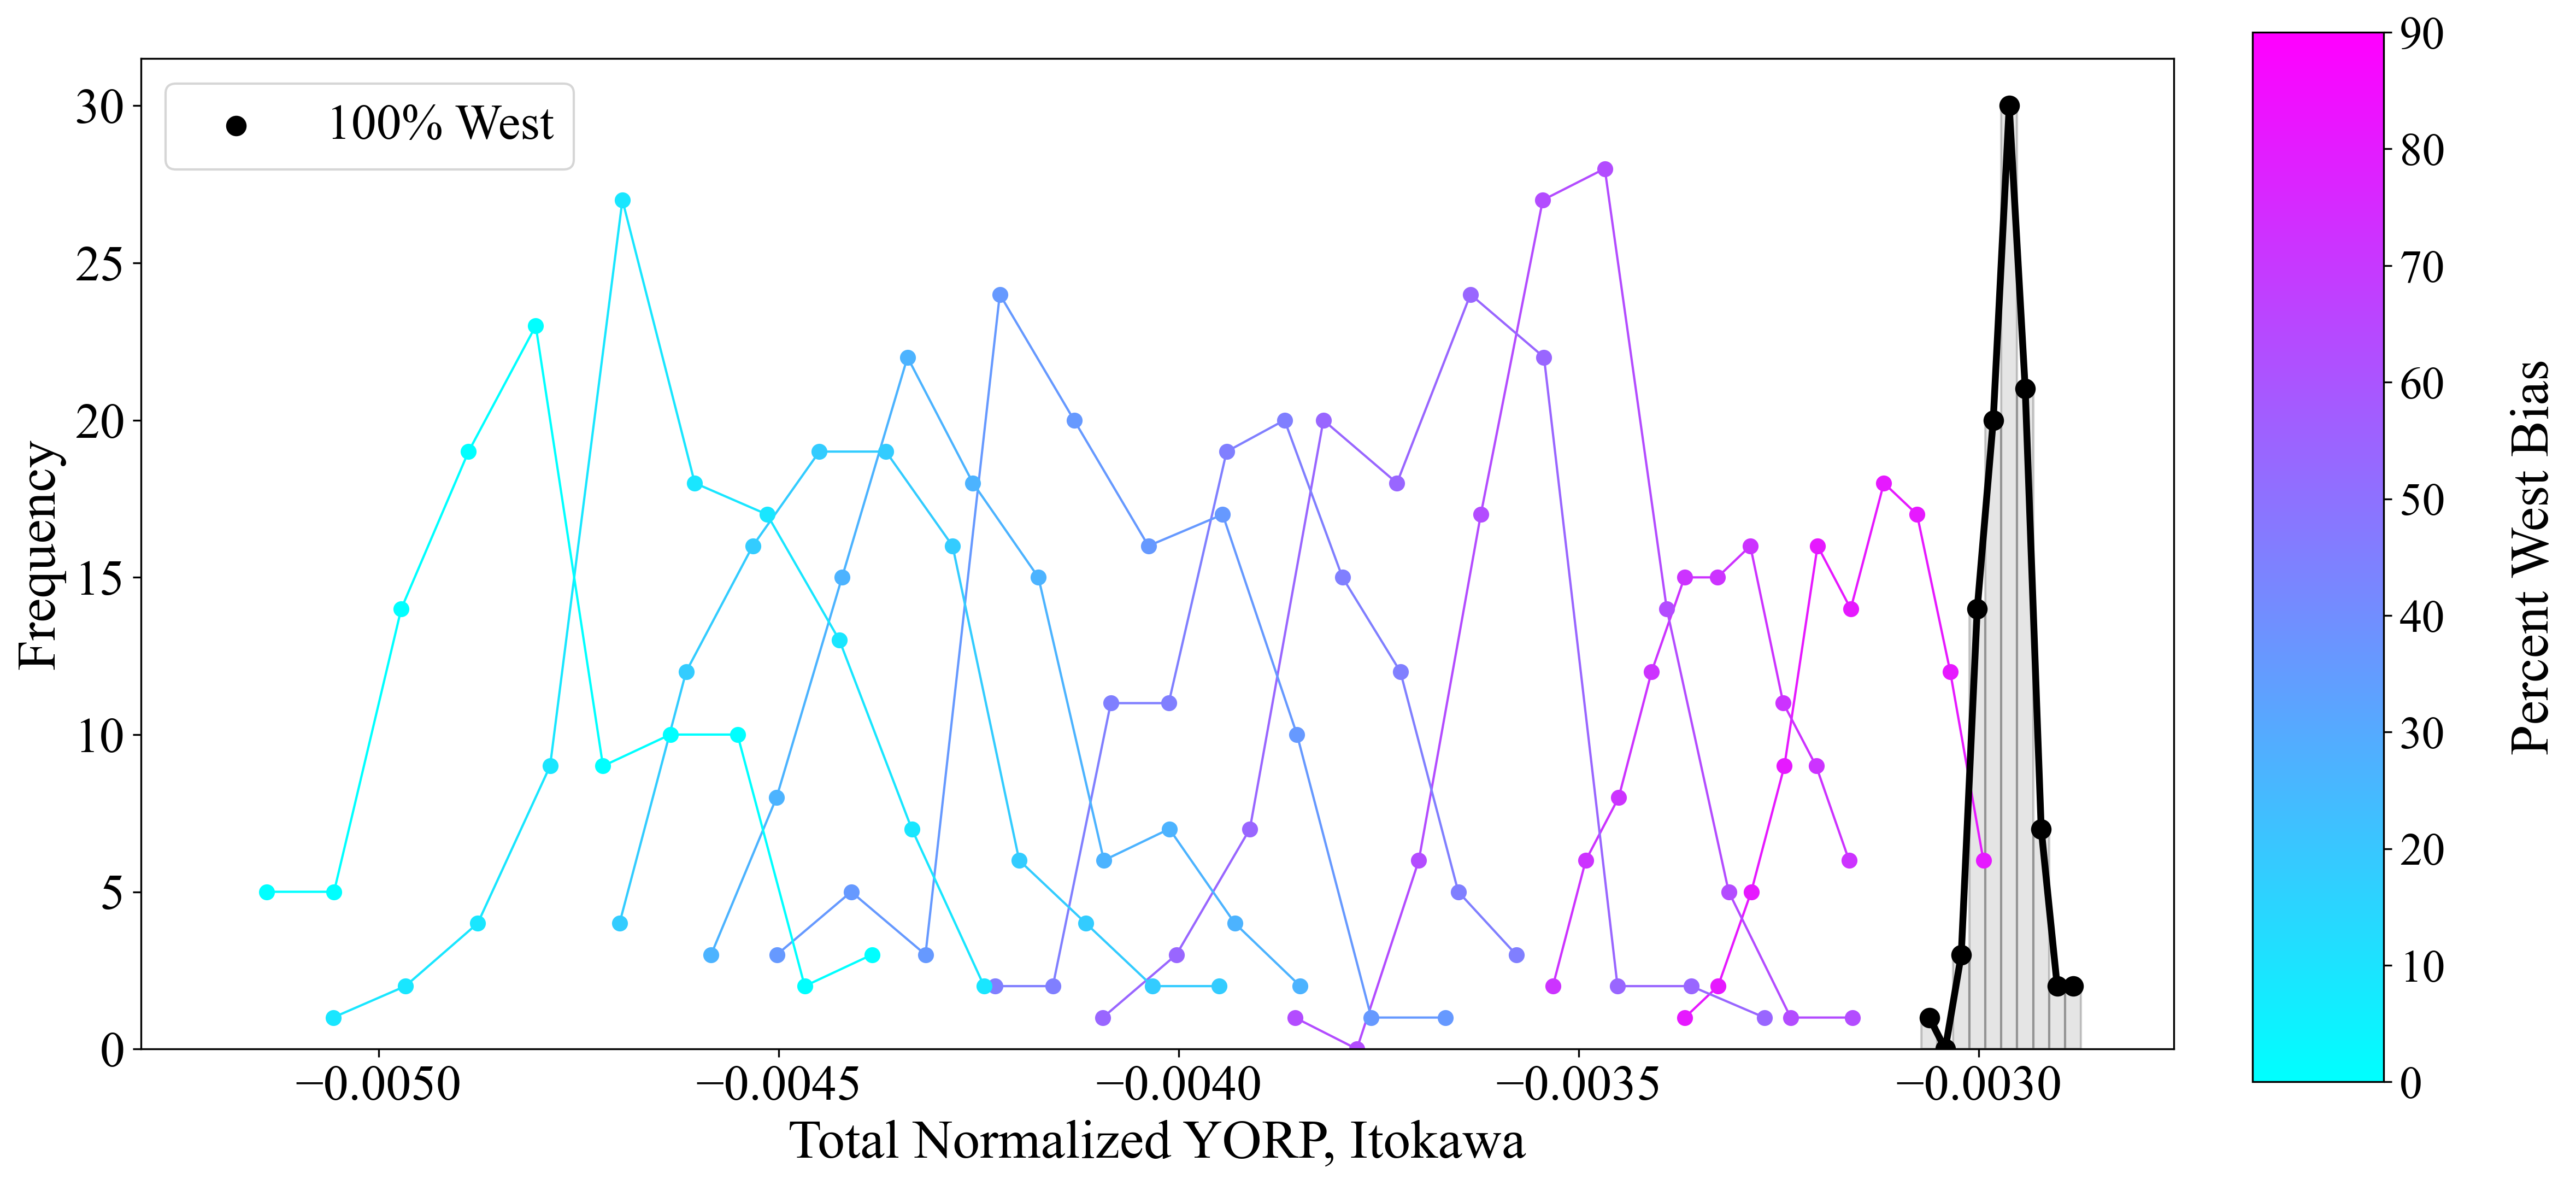
\includegraphics[width=\textwidth]{fig/itokawa_orient_samesize_recreate.png}
    \end{subfigure}
    \caption{Change in global YORP spin coefficient when enforcing a percentage of boulders with a westward orientation bias. Each profile is a histogram of global YORP spin coefficients. The black histogram represents the 100\% west bias for all boulders}
    \label{fig:orient_bias}
\end{figure*}

In surface observations of Bennu, preferential orientation of boulders was observed due to surface slope, where boulders aligned their long axes to the downhill direction of the local mass flow \cite{Tang2023}.Here we simulate varying degrees of orientation bias relative to local cardinal direction, ranging from 10\% to 100\% west-facing preference. This is done by evenly distributing boulders on every facet and enforcing a constant size of 1 m in diameter for each boulder, but choosing random individuals at the predetermined ratio to be pointing within 0.05 radians of directly west. We see that the average global YORP changes when 100 samples of boulder populations are simulated with the orientation bias enforced at each percentage level. The zero bias case is representative of a uniformly distributed random set of orientations for each boulder on the surface,and is therefore considered the control.

In calculating the averages associated with Fig.\ref{fig:polar_bias}, we see that the mean global YORP for both Bennu and Itokawa trends positive as boulders are biased to point westward. Bennu begins with a positive global YORP value and increases shallowly as west bias increases, whereas Itokawa begins much more negative and increases steeper with increasing west-pointing bias. A similar analysis can be done with eastward bias showing an increasingly negative contribution to boulder-induced YORP as more boulders align the dominant radiative face towards the spin direction.  We also see a shallower increase in Itokawa's total boulder-induced YORP, showing a higher inertia to westward orientation preference of boulders. This is due to the lower percentage of equatorial surface area on this body as compared to Bennu, where most facet normals align more strongly with the equatorial plane versus the z-axis.

Another possibility for bias is that of one large boulder shifting in the dominant re-radiation direction on the surface, such as in the case of mass flow alignment or fragmenting due to heat cycling. This will also change the global YORP torque in the direction of bias. As shown in section \ref{bennu}, just 1.6\% (or about 96 out of 6000) of the largest members of our base population are needed to model boulder YORP contributions and a single large boulder can be the driver of the most extreme edge cases. A change in the magnitude or sign of the torque vector of the largest boulders will have a proportionally large effect on the global spin. A large boulder is also unlikely to move, and will act as a static rudder of sorts, continuously changing YORP in a secular direction until it is removed, buried, or permanently shadowed. 


\subsection{Location Bias: Polar Migration}
\begin{figure*}[t!]
    \centering
    \begin{subfigure}{0.49\textwidth}
        \centering
        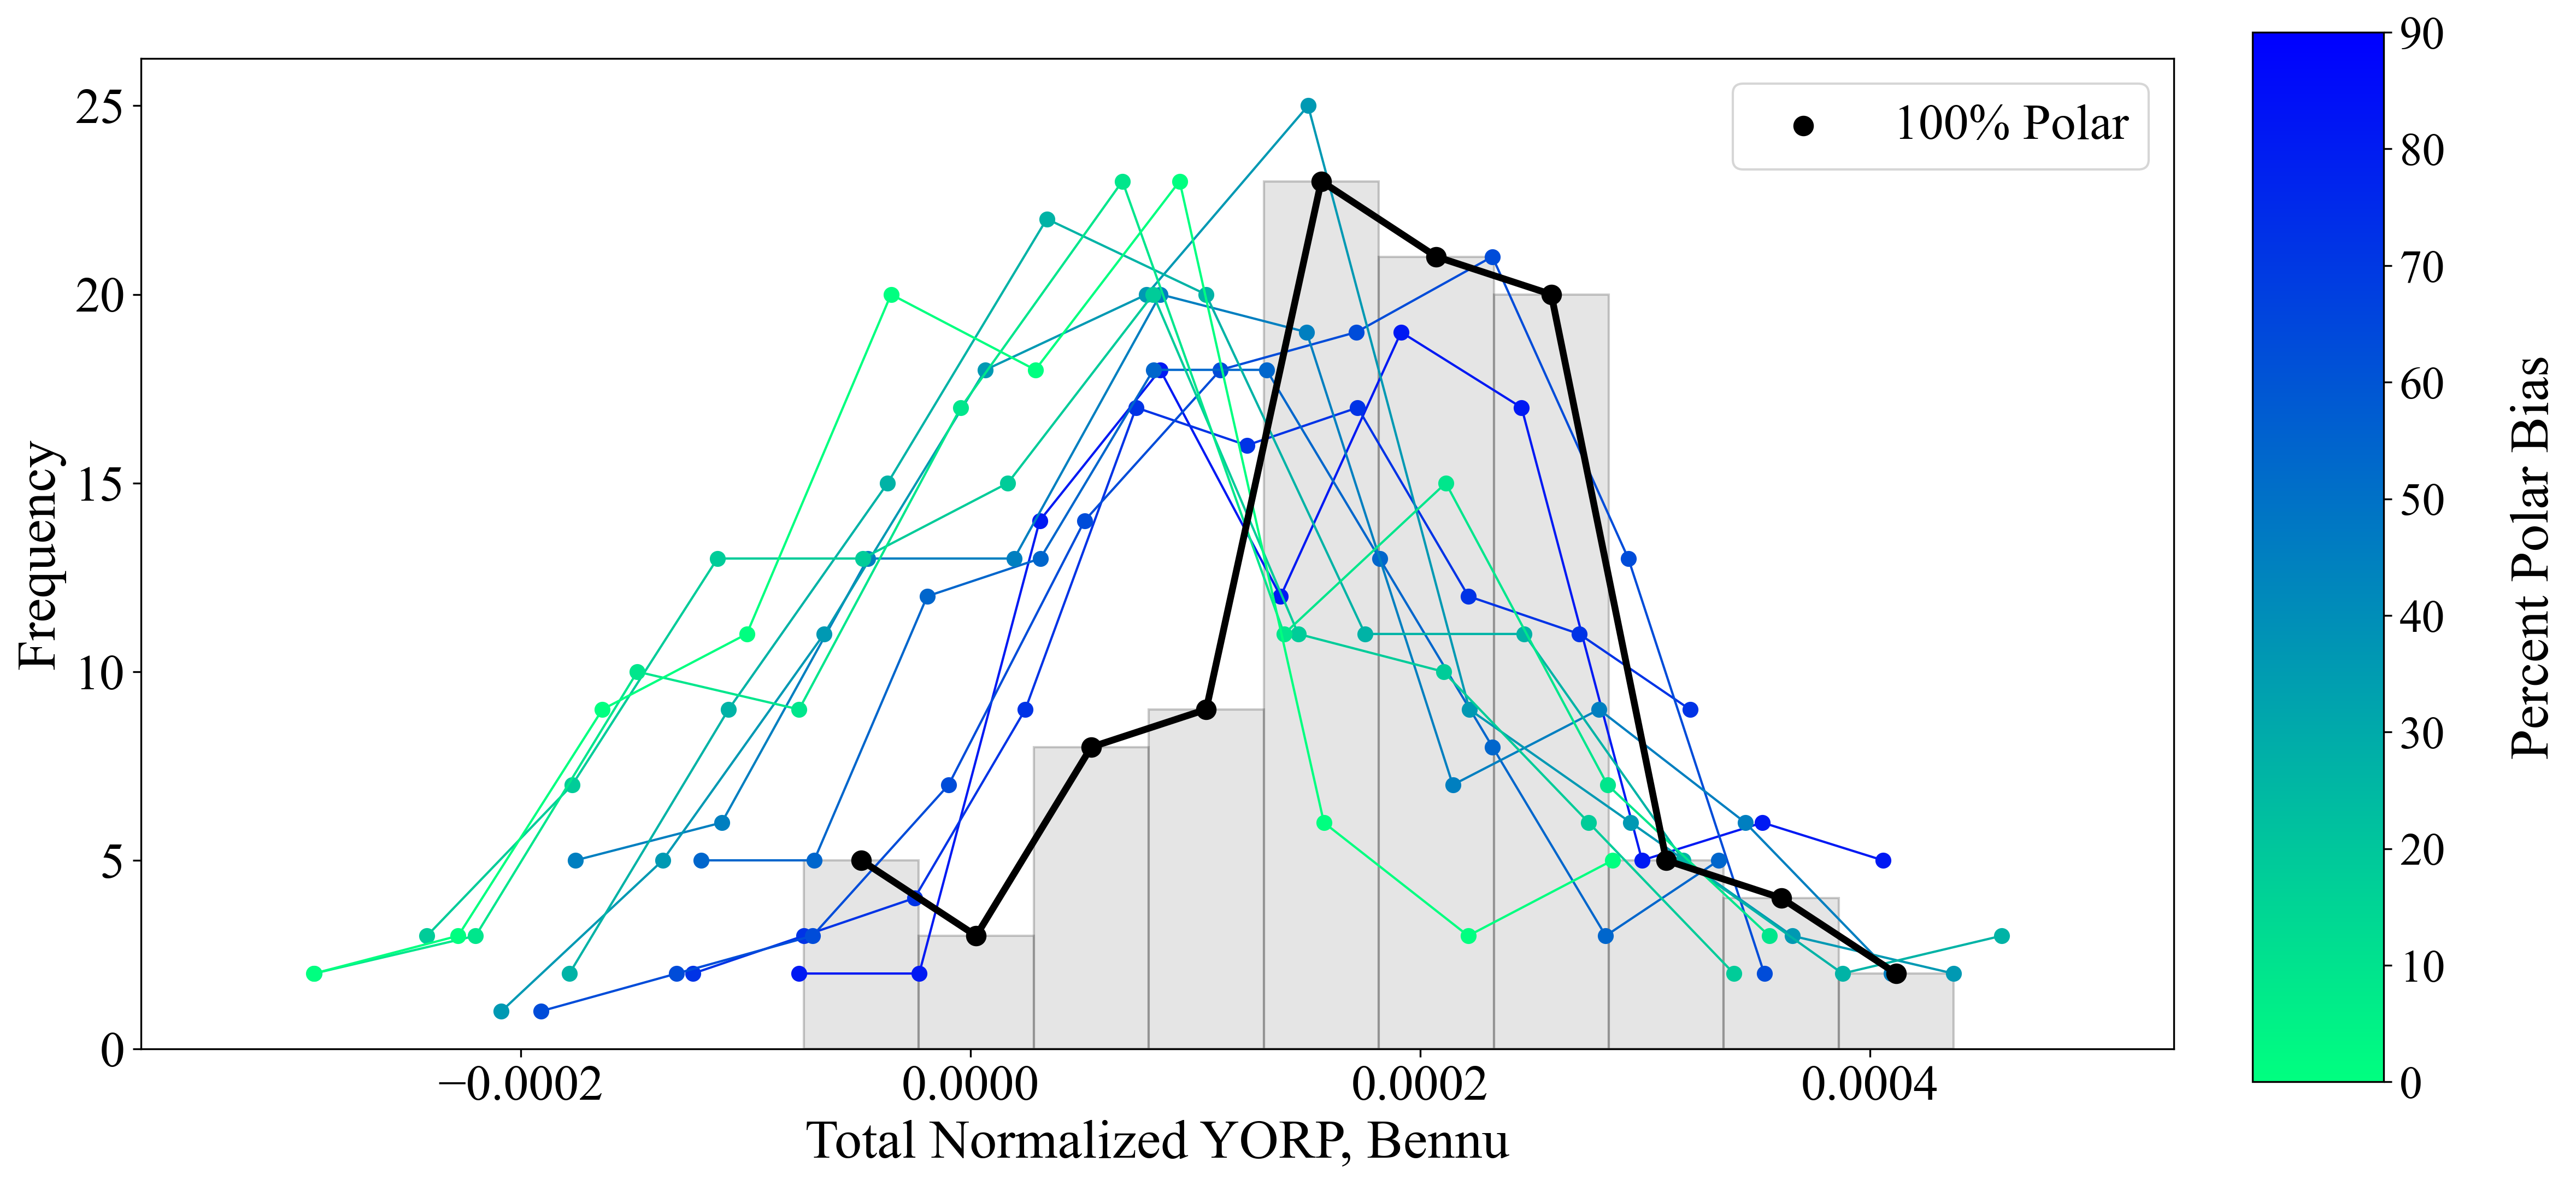
\includegraphics[width=\textwidth]{fig/bennu_polar_samesize.png}
    \end{subfigure}
    \hfill
    \begin{subfigure}{0.49\textwidth}
        \centering
        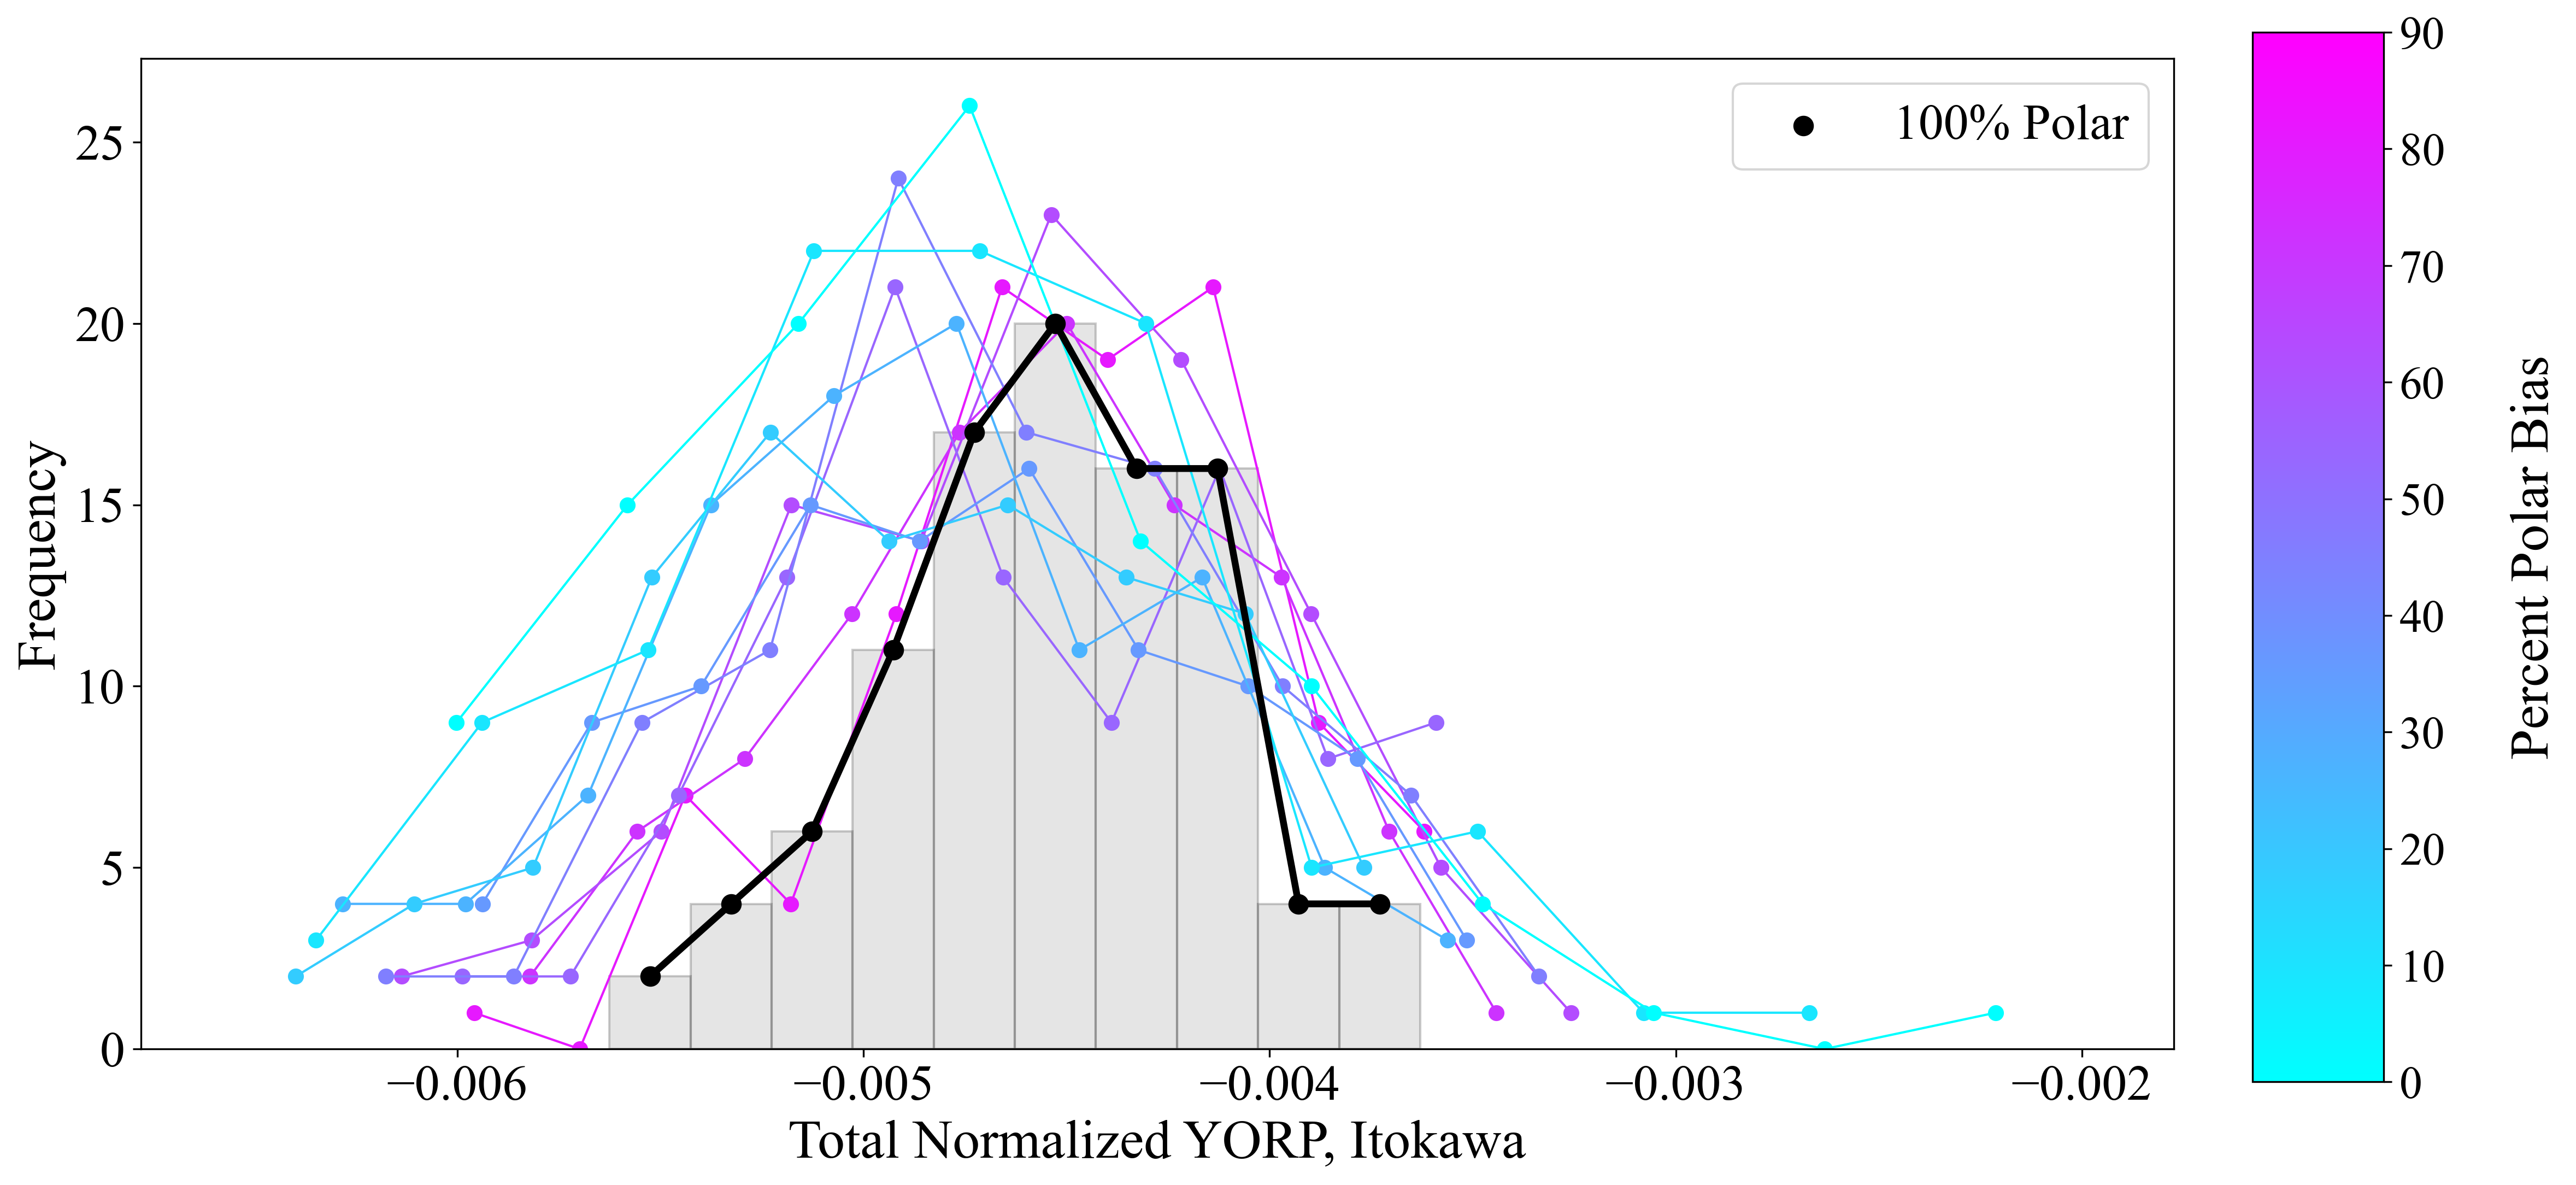
\includegraphics[width=\textwidth]{fig/itokawa_polar_samesize.png}
    \end{subfigure}
    \caption{Change in asteroid global YORP spin coefficients when removing boulders outside of $\pm 30^{\circ}$ latitude, varying the percentage until $100\%$ are outside of the the bounds equivalent to a liberal cushion about Bennu's Roche lobe}
    \label{fig:polar_bias}
\end{figure*}
The very old geological history of Bennu has been referenced to explain the variation in material composition as well as the distribution of boulders we see today. As Bennu migrated to it's current orbit, material migrated towards areas of high gravitational potential. This has caused the Roche lobe feature at the equator \cite{Scheeres2019}. To examine the conditions that caused this conglomeration of material, we bias boulder placement outside of the Roche lobe, or above and below $\pm$ 30 degrees latitude. This could also simulate boulders migrating to this area during an era of YORP spin-down, or the case of leftover boulders after larger ones have left the body through migration to the equator and reached escape velocity. The investigation of this configuration of boulders outside of the equatorial regions provides insight to how boulder-induced YORP changes as the surface redistributes material over time and eventually becomes what we see today. Future work will examine the gathering of boulders in craters or piling against larger gravitationally downhill features.

We simulated 100 cases of boulders on each shape model, with the number equal to facet resolution of the shape, with a varying percentage of bias in the location, similar to the process of inducing orientation bias. The random selection of orientation was kept consistently uniform while the size selection was standardized at 1 m in diameter. The distribution outlines in the top plot of Fig.\ref{fig:polar_bias}, in gradient colors of green to blue up to the 100\% polar bias case in black, have small variations in boulder-induced YORP as the bias increases. We see that the removal of boulders from the polar regions of Bennu moves the average in the positive direction and the lower bound of each distribution increases as the bias gets larger, but not as dramatically or linearly as seen with orientation bias. 

When performing the same analysis on Itokawa, we see a similar shift of the data mean in the positive direction. The lower and upper bounds of the 0\% bias case are the widest of any histogram shown, and the 100\% bias is the most constricted. One interesting feature of these results is that the distribution of 100\% polar bias on Itokawa is entirely negative boulder-induced YORP values. 

If we observed a large boulder closer to the pole of an asteroid, such as Bennu's large southern hemisphere feature, the implications on YORP evolution would be affected by induced prevention of material moving towards the equator by the damming effect this large feature will have on smaller, more dynamic particles on the surface. As material moves in mass flows, more regolith and small boulders will aggregate against the uphill of the large feature, increasing it's size and YORP contribution as well. This can serve to amplify the original YORP contribution of the large boulder until the local potential is overcome or the feature is somehow removed. Our bias analysis examines the case of one feature causing the collection of many, therefore increasing the presence of boulders in polar regions which would increase the YORP torque if the trend seen on Bennu and Itokawa follows for other prograde rotators in this size regime. Similarly, an large equatorial feature would be continuously buried by smaller particles moving downhill, and the YORP torque would be reduced as the feature is covered and smoothed. In these cases, as seen with increasing polar bias, we expect that YORP spin torque evolution will occur incrementally and predictably as the surface evolves unless a catastrophic disruption were to occur. 

\section{Total YORP Discussion}\label{discussion}
\subsection{Crater YORP}
Craters were observed on the asteroid Bennu with detail due to the hovering image survey carried out by the OSIRIS-REx mission \cite{Walsh2019}, the same survey from which our boulder population statistics were derived. Studying the crater population has opened investigations about the surface and its age. Specifically, studying craters informs how a proposed armoring factor has an influence on the presence of specific sizes of craters and allows for better characterization of resurfacing processes on rubble-pile bodies \cite{Bierhaus2022}.  The population was characterized and reported following shape modeling efforts \cite{Daly2020a}. The depth-to-diameter ratios are reported for 108 impact craters larger than 10 m in diameter.  We present here the calculated YORP contribution from the crater population on Bennu, according to Zhou et al.'s formulation. Their findings have shown that craters with depth-to-diameter ratios less than 0.05 can be ignored. For the most realistic case of surface roughness, craters can reduce total YORP torque by tens of percents \cite{Zhou2023}. 

\begin{figure}[H]
    \centering
    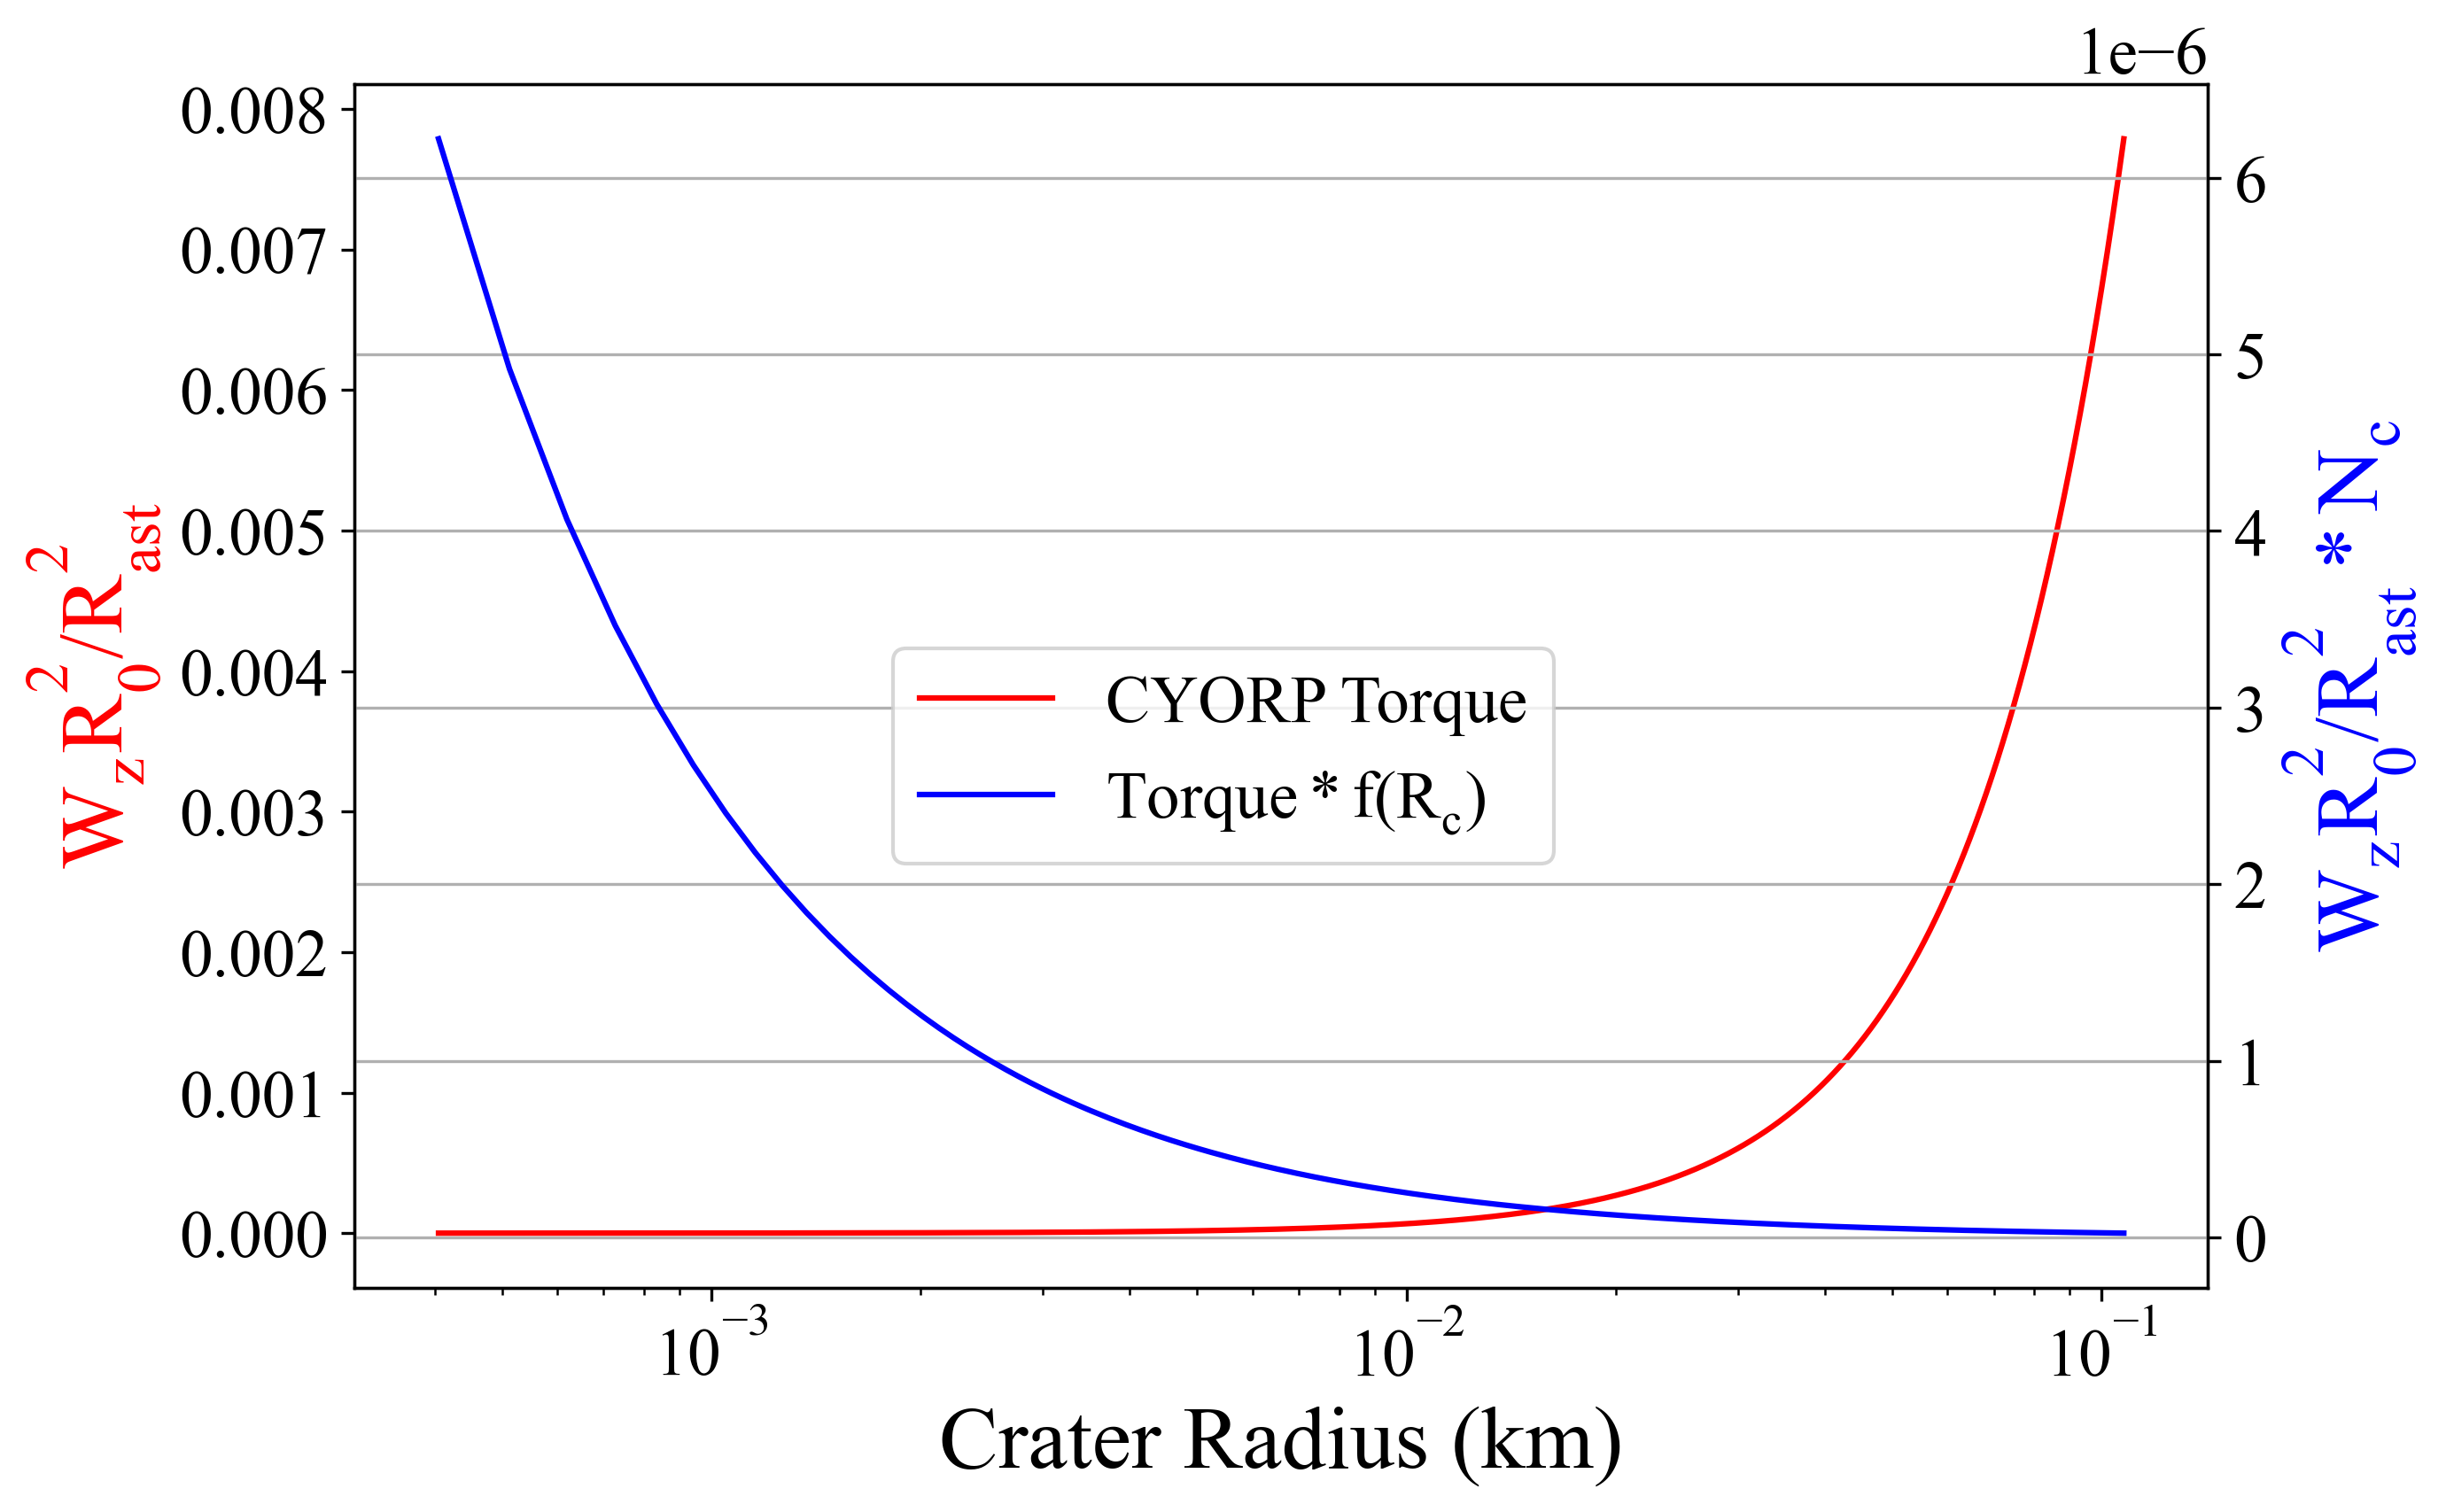
\includegraphics[width = 0.49\textwidth]{fig/cyorp.png}
    \caption{Normalized CYORP Contribution scaled by crater diameter frequency}
    \label{fig:three graphs}
\end{figure}

%now describe the figure you just added
For the size regime of craters on the asteroid Bennu, which stretches from 8 cm to over 200 m in diameter, we see an exponential relationship with how much a crater of a particular radius will contribute to the global CYORP sum. This data is provided by detailed analysis of Bennu surface maps which characterized the craters in order to age the surface material \cite{Bierhaus2022}. For comparison in blue, the torque is scaled by the prevalence of that size crater on the surface for an arbitrary body. We see that contributions of larger craters are tapered due to their lower frequency, while smaller craters could realistically dominate or negate the YORP forces of one large crater. This follows our power law distribution of boulder size and frequency. However, the difference in magnitude between the two y-axes shows that the limitations of the crater diameter power law reduce total CYORP torque by a factor of roughly one thousand. CYORP differs from normal YORP because it considers the thermal reabsorption that is specifically induced by a concave structure inclusive of self-shadowing and self-heating. For the spin-inducing component, we show a plot of magnitude of torque related to crater diameter, though there are other position factors that can make the torque either pro- or anti-spin, which varies the sign of the torque. 

According to semi-analytical models, a crater in this capacity is defined as the difference between flat ground and the depression of a crater. At specific sizes above the shape model resolution, these craters would be captured in the normal YORP calculation when this analysis is done as a sum of polyhedral facets. The same is true for very large boulders, and this will be discussed in the next section. Crater YORP is important to include in full discussions of the YORP effect of highly detailed surfaces and we go on to compare to other sources of YORP that have been shown.

\subsection{Tangential YORP}
Tangential YORP is the by-product of the thermal inertia of protruding asteroid surface material. As heat is absorbed over a day, it is transferred through the volume at a rate determined by it's mineral properties and geometry, summarized as the heat conductivity length, $L_{cond}$. This length is determined from analysis shown by Golubov \cite{Golubov2012}. 
\begin{figure}[H]
    \centering
    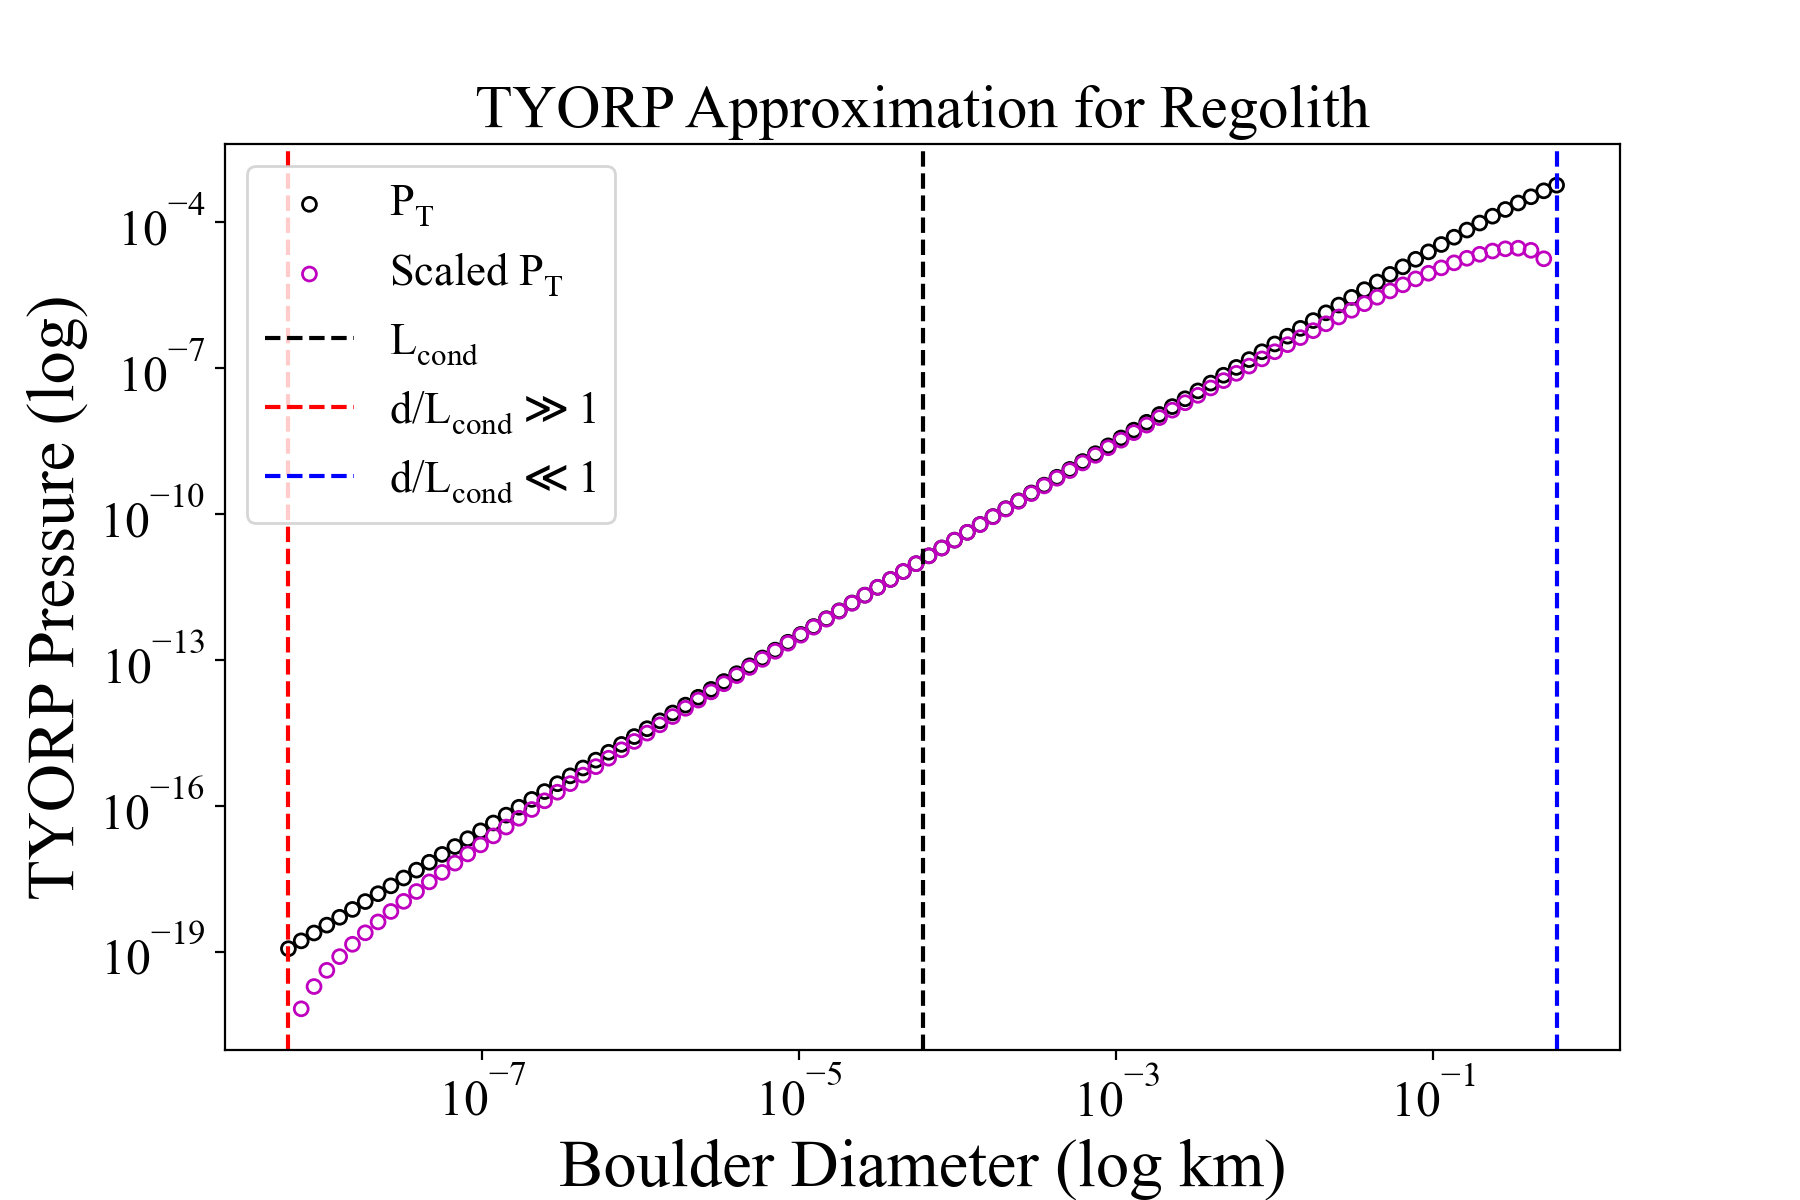
\includegraphics[width=0.48\textwidth]{fig/tyorp_regolith.png}
    \caption{Incorporating the assumption of smooth transitions below and above the ideal thermal inertia length, $L_{cond}$ with a logarithmic scale factor}
    \label{fig:tyorp_regolith}
\end{figure}

Varying types of material have different thermal inertias, and asteroids can have clustered features with similar thermal properties such as Bennu's concentration of high thermal inertia regolith at the Roche lobe \cite{Rozitis2020}. Tangential YORP is negligible or non-existent if the boulder diameter is so thick that energy is not propagated entirely through. Conversely, there is no force if the diameter is small enough to approximate instantaneous heat transfer and equal temperatures on each opposing face. With equal faces opposing, the YORP spin torque is averaged to zero. 

Here in Fig.\ref{fig:tyorp_regolith}, we show the magnitude of dimensionless TYORP pressure as it relates to boulder size when approximated as a flat wall. In this calculation, the wall thickness is equivalent to the boulder diameter. We have also scaled the analytical form of TYORP to consider the declination in strength at the bounds far away from the heat conductivity length. This logarithmic scale factor considers $d/L_{cond} = 100$ as an upper bound, and $1/100$ similarly as the lower bound for effectiveness.
Tangential YORP is known to impart positive rotational acceleration in most cases. What is presented here is a large variability in boulder-induced YORP. If any body has features that cause a preferentially negative normal YORP and boulder-induced torque and that same material falls within the bounds of thermal inertia necessary to induce TYORP, than the resultant spin could be non-accelerating. Golubov notes this may be the reason for a lack of observed YORP deceleration from the asteroid Itokawa, despite normal YORP calculations providing a small negative torque. With the additional consideration of boulders and craters, the sources of uncertainty grow and estimates of YORP must encapsulate this variability \cite{Golubov2012}. 

In comparing all the current models for YORP torque, we apply the obliquity-dependent TYORP equations from Ševeček which is also expanded upon in further works \cite{Sevecek2016} \cite{Golubov2019}. We use the expression in Eq.\ref{eq:tyorp} which considers obliquity ($\epsilon$), number of boulders ($n_0$), the sign of angular velocity ($sgn(\omega)$), and a boulder size power index of 3. 
\begin{equation}\label{eq:tyorp}
    \begin{split}
    {T_{z,}}_{TYORP} & = 4.5 \frac{\Phi R^3}{c}n_0 \mu \exp \Bigg( -\frac{(ln(\theta)-ln(\theta_0))^2}{\nu^2}\Bigg)\\
    & \times (1+cos^2\epsilon)sgn(\omega)
    \end{split}
\end{equation}

\subsection{Overall YORP Comparison}


The aim of this work is to characterize sources of YORP torque from small features that border the size limits of regolith as well as the maximal surface resolution obtainable from ground observations. By expanding the YORP torque model in this way, it could be possible to make better estimates of YORP from rough radar shape models. We have varying levels of shape model resolution for the asteroid Bennu and each one comes with a different YORP torque evaluation based purely on the geometry of the surface and it's orbit. Here with Fig. \ref{fig:all_yorps} we see the the relative strength of different YORP torque sources and their uncertainties when applied to the case of Bennu. The normal YORP in red corresponds to our analysis of the shape without boulders, and the BoYORP mean and upper bound (in yellow) correspond to the results of our statistical study, $\mu+1\sigma$ to show variation in log space. The crater YORP model, shown in blue, is reported from Zhou and shows the variation  of depth to diameter ratios that one would expect to be the upper and lower bounds of the largest crater on Bennu ($h/D_0 = 0.1\pm0.03$) \cite{Zhou2022} \cite{Daly2020a}. We also report the observed YORP values from HST and their error bounds in green \cite{Nolan2019}.

\begin{figure}[H]
    \centering
    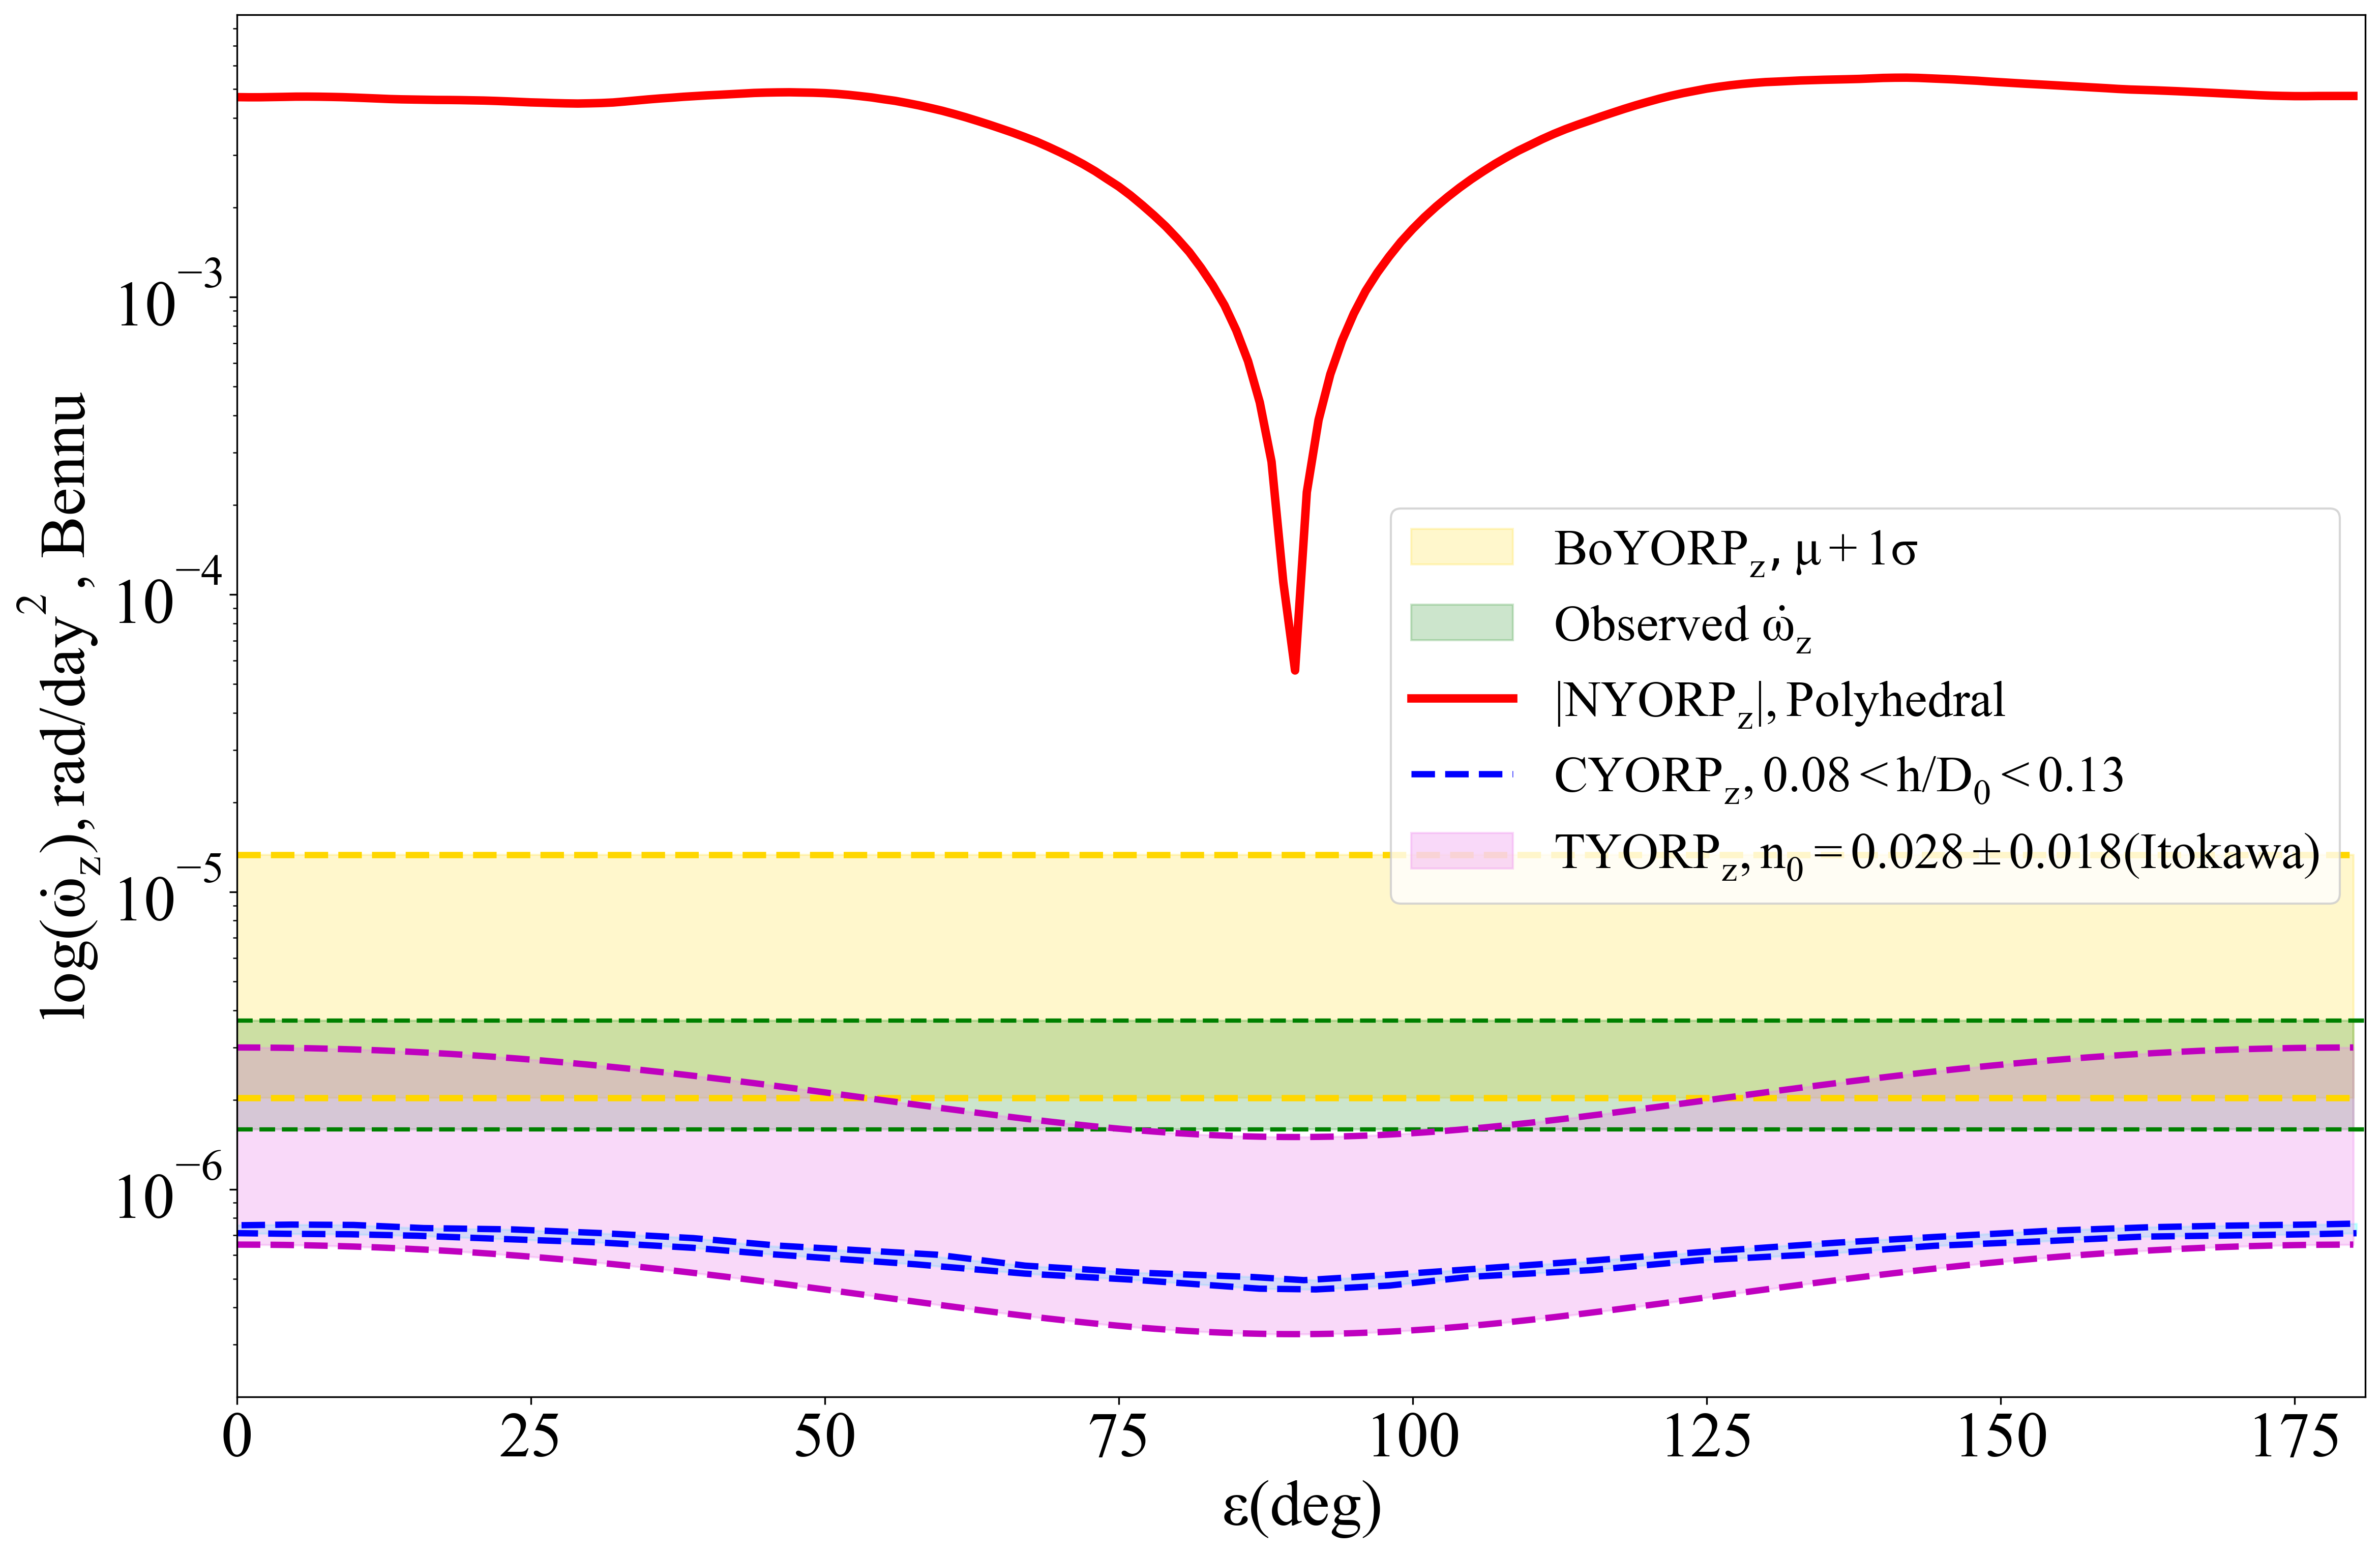
\includegraphics[width=0.49\textwidth]{fig/all_yorps.png}
    \caption{Comparison of analytical YORP spin components for Bennu as a function of obliquity}
    \label{fig:all_yorps}
\end{figure}
Tangential YORP in this formulation comes from Golubov and shows that, even without enforcing the size boundaries of effectiveness, we still see a small relative contribution from this effect \cite{Golubov2017}. The bounds reported here correspond to the error in the variable $n_0$, an approximation for surface area covered by boulders. The values reported for $n_0$ of Itokawa are $0.028\pm0.018$ and contain the variability reported in violet in our figure. Here we make the assumption that Bennu and Itokawa have similar boulder populations and therefore the same error in $n_0$ can be applied to Bennu. We also assume that the mean boulder YORP value reported at zero degree obliquity is applicable at all obliquities if not larger. Boulder-induced YORP is the strongest influence in this comparison and while here we show the mean value of spin acceleration from our simulations, the largest cases are 2 to 3 orders of magnitude larger than the BoYORP mean for Bennu. In the log scale, we only represent the positive contribution of boulder-induced YORP, but we recognize that there is an equal possibility that we contribute a strong negative acceleration to the spin of the asteroid. This is not true for the models of crater and tangential YORP shown, which are analytically positive at all obliquities. 


When considering the sources of uncertainty from each model of YORP spin torque, we can compare them in magnitude and combine them to report a total YORP uncertainty including the variability due to boulders. Included is the uncertainty due to shape model resolution, reported as the difference between the YORP torque calculated from a high-fidelity model and one calculated from the $~$6k facet degraded Bennu shape model. We follow a root-square-sum procedure. 

\begin{equation}
    \sigma_{total} = \sqrt{\sigma_{BoYORP}^2 + \sigma_{TYORP}^2 + \sigma_{CYORP}^2 + \sigma_{NYORP}^2}
\end{equation}

The error reported here is taken from the models shown in Fig.\ref{fig:all_yorps}, and the normal YORP error is extrapolated from the difference in YORP results in high and low resolution shape models of Bennu. This represents the variability due to the base shape. Boulder YORP error is the standard deviation from Fig.\ref{fig:cases_w_boulders}. Tangential YORP and crater YORP have upper and lower limits with an associated standard error within that variability. The total YORP uncertainty is $\num{1.394e-05}$ deg/day$^2$.

\begin{figure}[H]
    \centering
    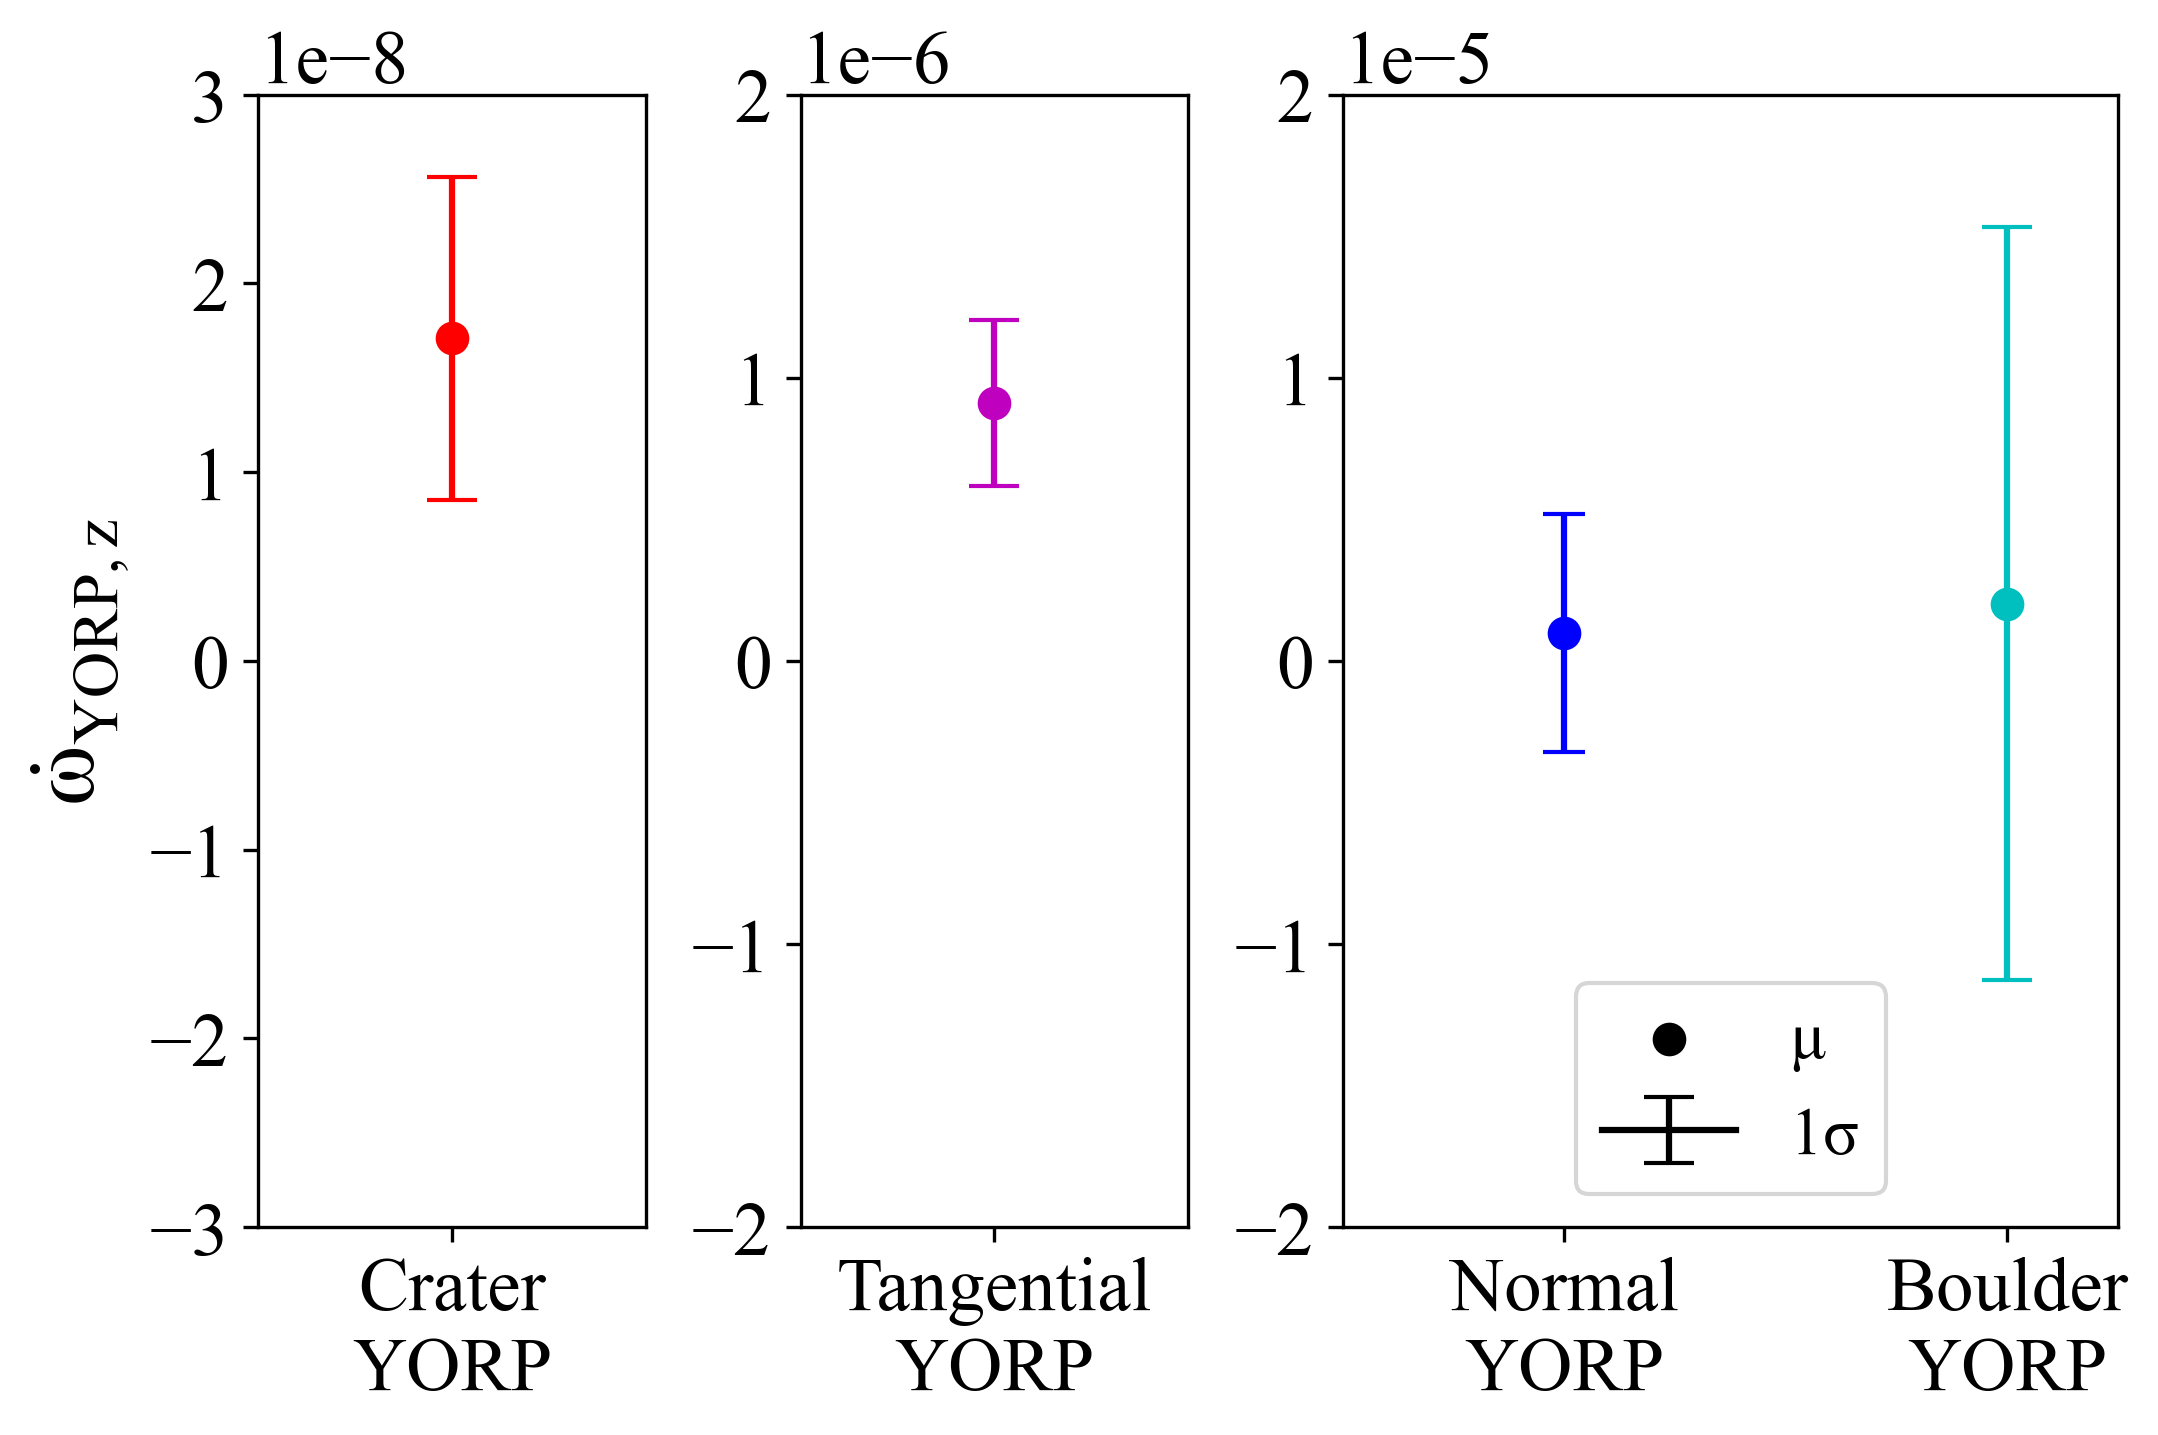
\includegraphics[width=0.49\textwidth]{fig/error_compare.png}
    \caption{Comparison of mean and standard deviation from several YORP models}
    \label{fig:err_comp}
\end{figure}
\section{Application to YORP Estimates}\label{implications}

As we consider tangential and feature YORPs from craters and boulders, this provides additional sources that could match ground estimates to actual in-situ measurements. For example, comparing pre-mission estimates of Bennu's YORP torque to the actual measurements from the OSIRIS-REx mission, we can map discrepancies due to resolution changes and unobserved features \cite{Nolan2019}. Another example is the lack of an observation of YORP from Itokawa. After mapping the surface, evaluation of the detailed model shows an expected YORP of $-2.5$ to $-4.5 \times 10^{-17}$ rad/s$^2$ from the geometry alone \cite{Scheeres2007a}. The YORP acceleration has also been calculated for Ryugu shape models with considerable uncertainty between 20 variations of the Hayabusa2 map results, $(-6.3$ to $-0.42) \times 10^{-6}$ deg/day$^2$ \cite{Kanamaru2021}. Their analysis varied the shape modeling method, stereophotoclinometry (SPC) or Structure-from-Motion (SFM), as well as the set of source images by day. Their requirement for shape model resolution was 49,000 facets. 

The standard error for Ryugu's YORP acceleration would be $1.47 \times 10^{-6}$ deg/day$^2$, which 10 times smaller than the total YORP uncertainty we derived from the combination of models for Bennu. The bodies are not extremely different in size or in the YORP observed or estimated for them. The uncertainty for Ryugu was derived from variation in shape model resolution, however, our uncertainty incorporated the expected contributions from boulders, craters, and tangential YORP. This shows the need for further consideration of the YORP impact from expected features and roughness and more complex thermal radiative patterns. 

\section{Boulder Motion}
%here Jay said to do some boe calcs
When the dynamics change, there can be new forces at the surface that induce boulder motion. This can be sliding, rolling, or escape that are all side effects of spin acceleration. Here we will show the difference in YORP spin torque contribution between a boulder at a single constant longitude, but varying between +45, 0, and -45 degrees in latitude. These are the same size (0.1m diameter) and orientation (directly west). The difference in torque between these boulders is equivalent to the change in dynamics due to a boulder moving from it's original location to a new one. In Fig. \ref{fig:motion_nodelta}, we show the YORP spin acceleration values for boulders at varying latitudes between -90 and 90 degrees, or south to north pole, that are all constrained within -173 and -178 degrees in longitude. Note that the distribution shows that boulders, all facing 100\% west with their dominant face, can vary between negative and positive YORP spin acceleration even on the same hemisphere. The boulders closer to the equator contribute the most spin torque due to the longer lever arm length from the central spin pole. However, slight variations in the tilt of the base facet can cause these swaps from positive to negative on boulders close to each other. 

\begin{figure}[H]
    \centering
    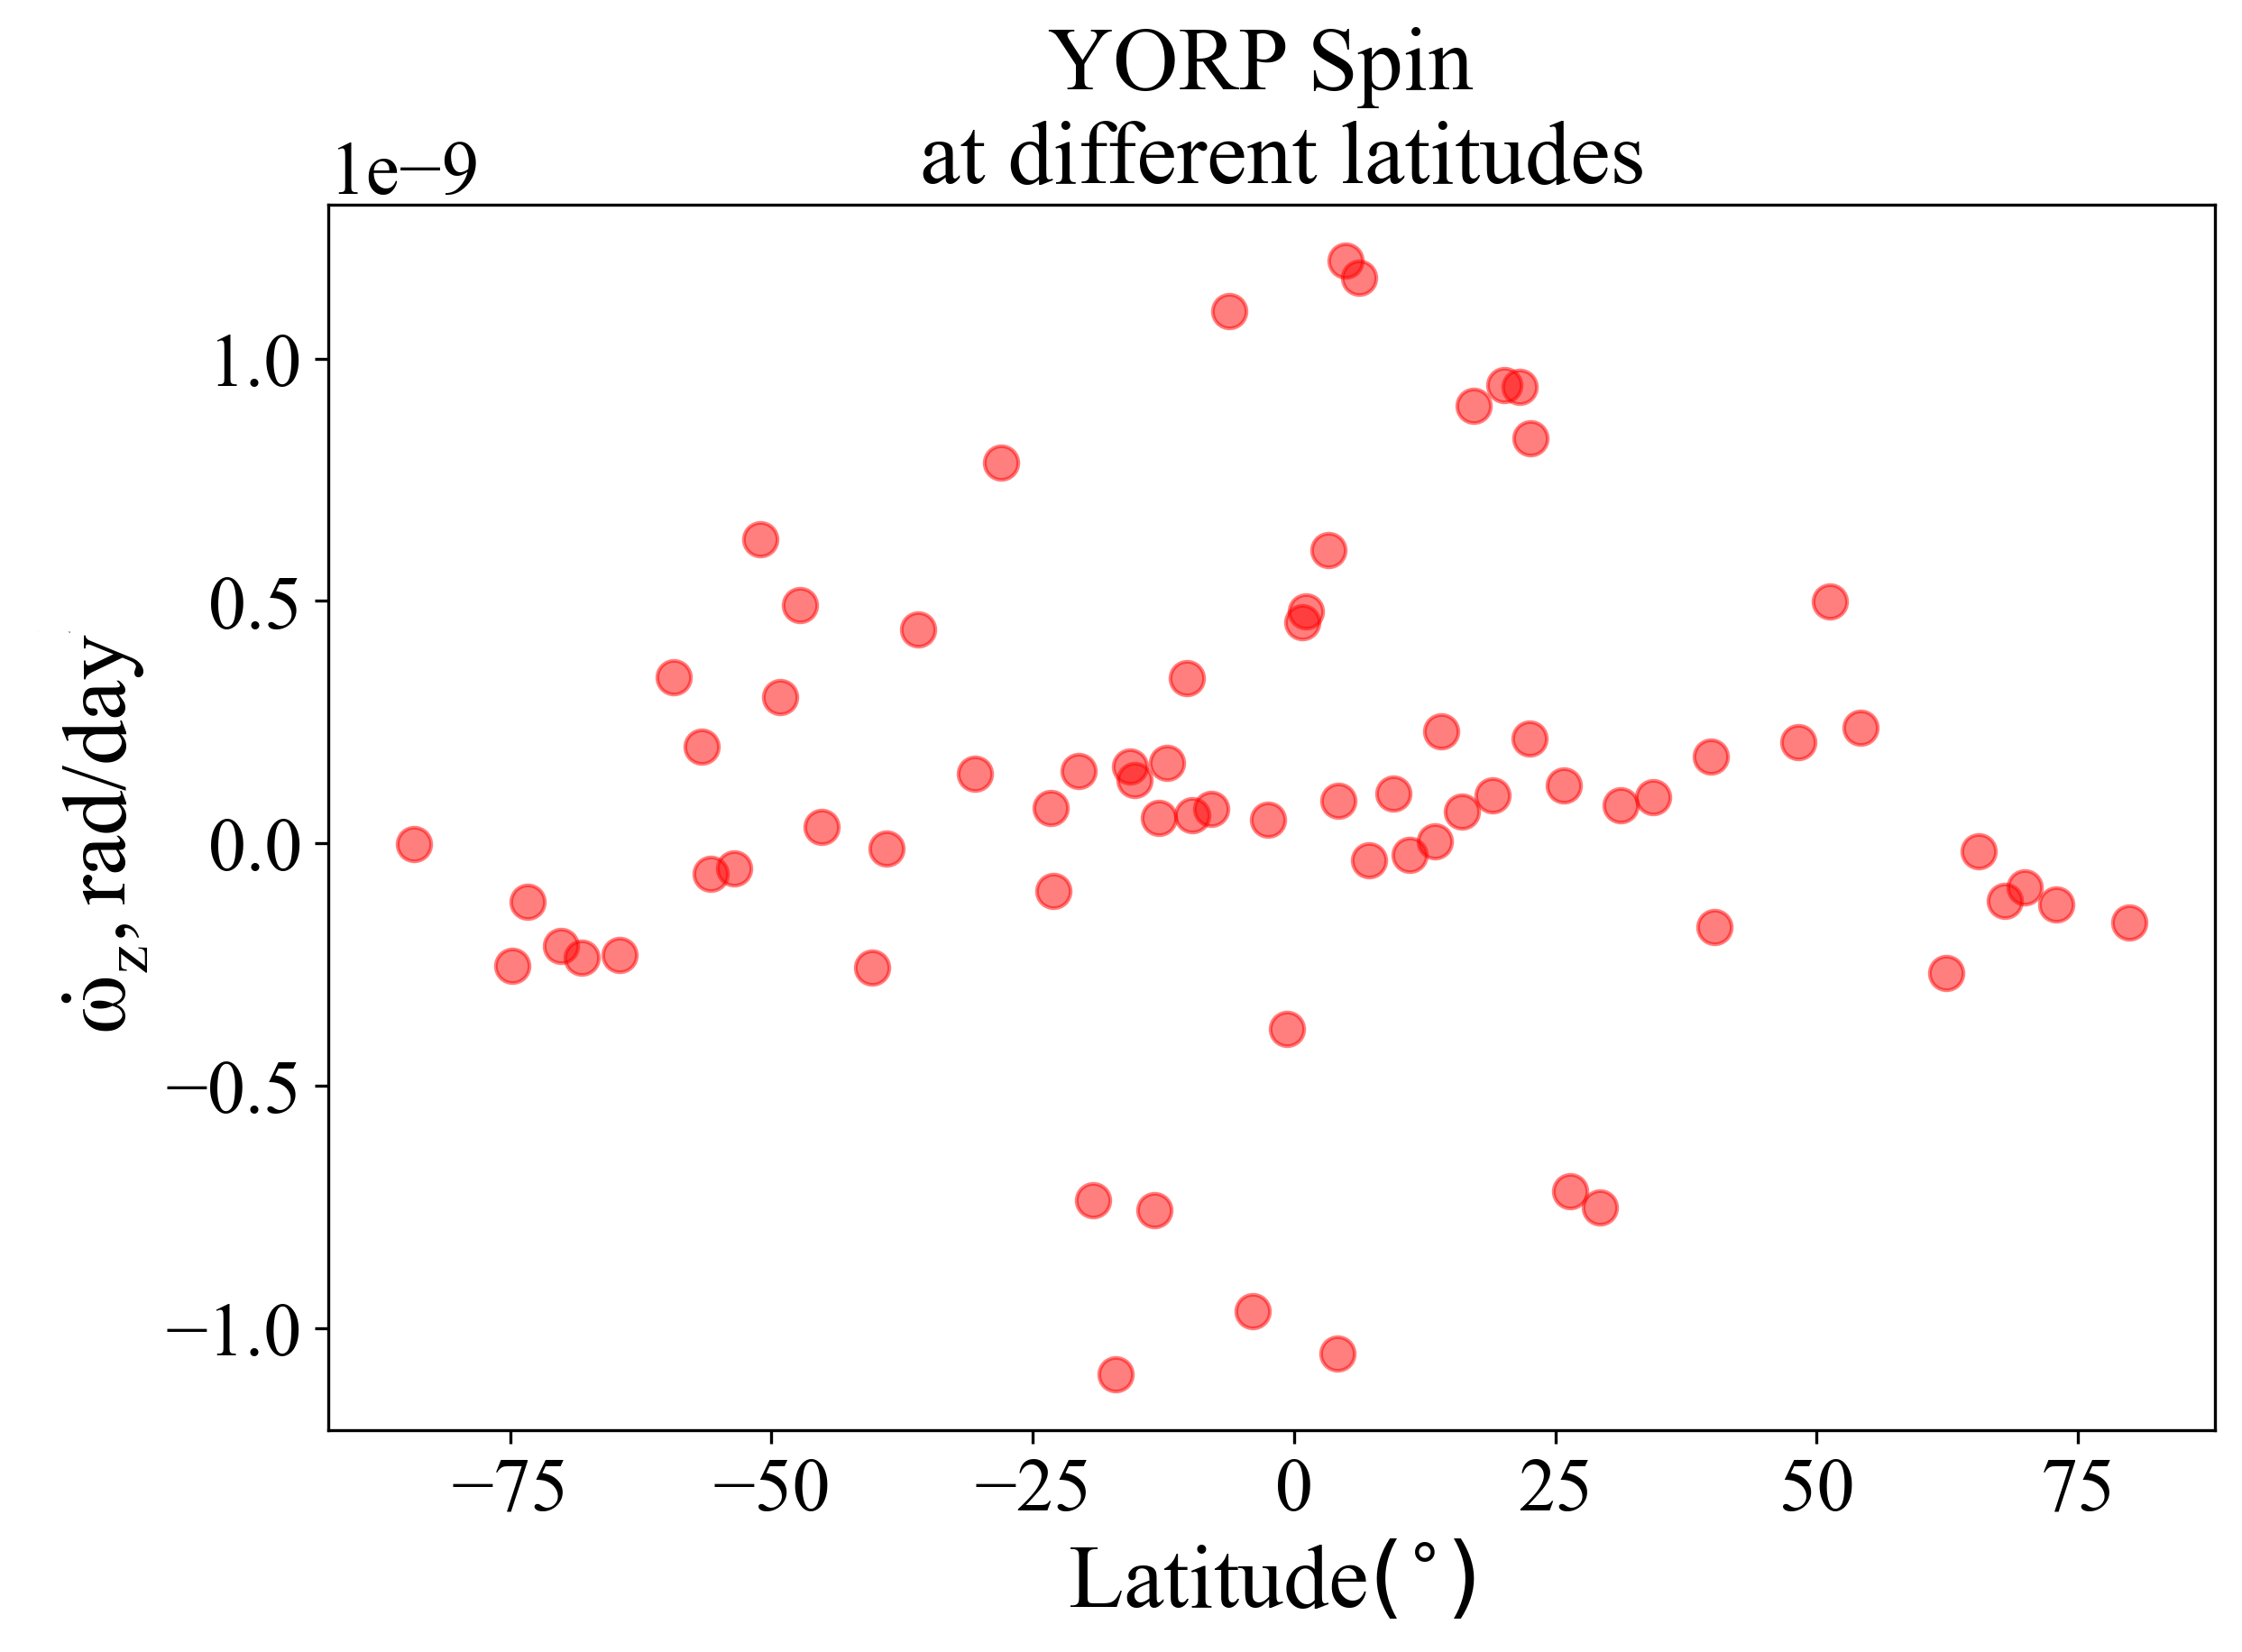
\includegraphics[width=0.5\textwidth]{fig/yorp_amt_boulder_motion_bennu.png}
    \caption{Differing amounts of YORP spin acceleration for boulders within 5 degrees in longitude but varying latitudes}
    \label{fig:motion_nodelta}
\end{figure}


We show the delta distribution of these boulders, in Fig.\ref{fig:motion_delta}, by taking the difference of YORP spin from each boulder compared to it's closest north neighbor. The change in latitude varies by boulder comparison, and we show the resultant change in YORP acceleration contributions based on this latitude change. Note that the maximum delta in longitude is just 5 degrees. There is no relationship between larger latitude change and YORP acceleration change. The motion represented by $0-2^{\circ}$ of latitude change is the most common and shows the largest distribution, positive and negative, of YORP acceleration change. 

\begin{figure}[H]
    \centering
    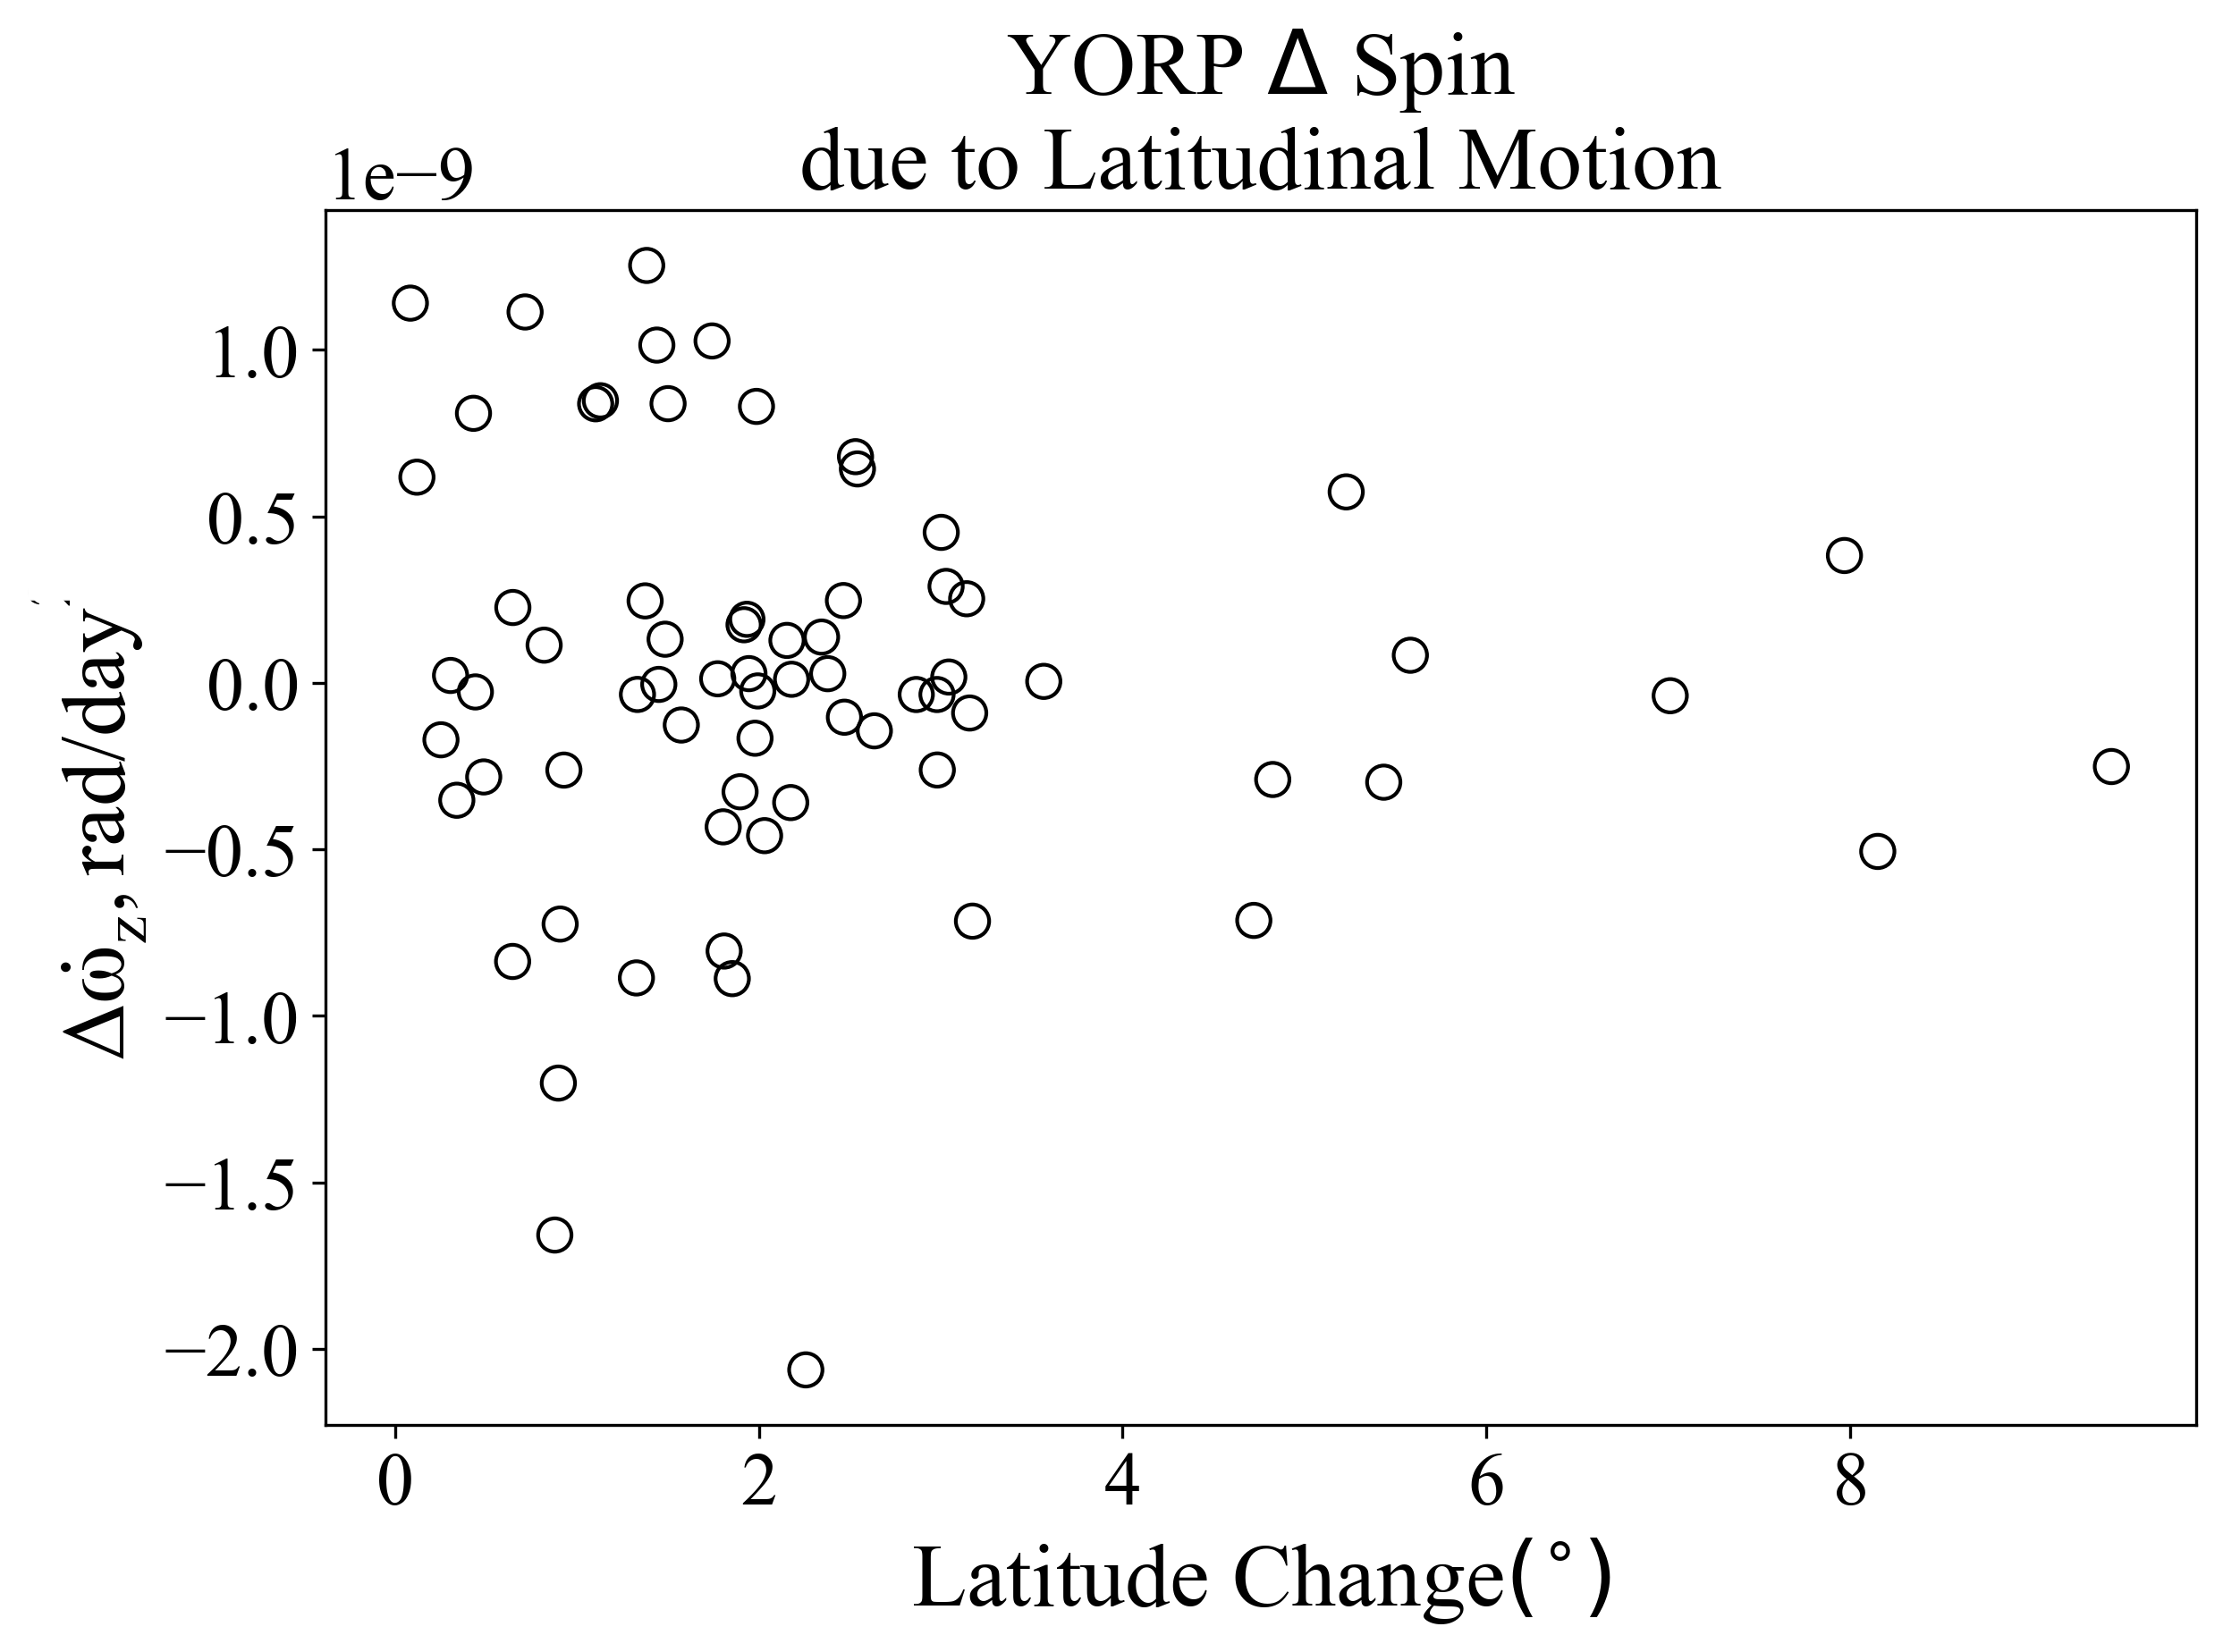
\includegraphics[width=0.5\textwidth]{fig/yorp_delta_boulder_motion_bennu.png}
    \caption{The change in YORP spin acceleration from boulder motion with the latitude degree change shown on the x-axis}
    \label{fig:motion_delta}
\end{figure}

This data shows how much YORP can change from the same size, same orientation, and same shape of boulder being assessed at different locations, mainly varying in latitude which is the larger driver of YORP spin acceleration change due to the lever arm length variation. The largest YORP spin acceleration delta is $1.6828\times 10^-9$, which is equivalent to a doubling rate for Bennu of 76 million years from a single boulder delta. If extrapolated to the case where 1\% of the boulders on the surface, now sized at 1m, were all to increase in YORP acceleration at this rate, then the doubling time due to just these boulders is now ~153,000 years. In the Bennu lifetime, this is a short period for accelerating from a 4.3 hour period to 2.15 hour period. In the next chapter, we will show the rotational deformation speeds for these asteroids and compare these values to what we have found here.





\section{Summary of Spin Evolution Findings} \label{conclusion}
Boulder-induced YORP is the consideration of larger-scale surface roughness which can still be modeled through facet geometry therefore is not captured in regolith roughness approximations. We have shown that compared to the magnitude of other analytical models of YORP, it is a significant contributor to final magnitude and uncertainty. We can use this characterization of YORP from boulders to inform future estimates of measured YORP versus actual shape, which aims to clarify the sources of uncertainty or bias in our current YORP estimates. Simulating realistic populations of boulders provides an applicable way to tie together observation and modeling of YORP in a way that purely analytical models have not.

\begin{itemize}
    \item The mean boulder addition to YORP-induced spin acceleration on Bennu was $.1039 \pm \num{1.329e-5}$ deg/day$^2$, and $\num{-2.129} \pm \num{1.717e-5}$ deg/day$^2$ for Itokawa.
    \item Boulders contributing more than 1\% to global YORP on Bennu were 18\% more likely to be found within 30 deg. of the equator and 29\% more likely to point west or east. Those values for Itokawa were found to be 9\% and 3\%, respectively. 
    \item The average size of boulders that contribute more than 1\% to Bennu's global YORP spin acceleration was 4x the full population mean, and 15x larger for Itokawa.
    \item The mean of total global YORP spin increased an average of $7.913 \pm \num{0.574e-7}$ deg/day$^2$ with each 10\% increase in westward orientation bias for Bennu, and $1.029 \pm \num{0.110e-6}$ deg/day$^2$ for Itokawa.
    \item In the case of biasing boulders location towards the polar regions (outside of $\pm 30^{\circ}$ latitude), the global YORP spin increased an average of $2.262 \pm \num{3.052e-7}$ deg/day$^2$ with each 10\% increase in polar bias on Bennu, and $1.471 \pm \num{3.973e-7}$ deg/day$^2$ for Itokawa.
    \item The change in average of the global YORP spin acceleration when boulders $< 1$ m were removed was 1.11\% and 1.36\% for Bennu and Itokawa, respectively.
\end{itemize}

The TYORP effect is considered for it's part in the larger YORP model, but acknowledged for it's bounded contributions. We have analyzed the relationship between meaningful and observable aspects of boulders, such as dominant orientation, placement, and size, and the amount of re-radiative thermal torquing which will provide possible avenues for explaining specific routes in YORP evolution over time. In discovering the statistical contributions of varying sizes of boulders on two asteroid models, we have shown that boulders less than 1m make up 90\% of the YORP estimate despite being 1\% of the total population of boulders. Capturing this level of detail in such a small portion of the population allows for further work to continue analyzing the dynamical impact of the presence and motion of larger, more observable boulder candidates. 

We have compared the relative strength between the CYORP model and the contribution due to additional boulders. Craters experience self-shadowing and bouncing radiation and absorption and this behavior requires it's own specific semi-analytical model. To extend the complete analytical YORP model, we present here an extension of normal YORP applied to new small-scale geometries in the form of boulders. When analyzing asteroids visited in the future, we can use these results to make reasonable estimates on YORP from possibly incomplete or low-resolution shape models, such as ones obtained from flybys or impacts.

We have also analyzed the conditions under which consistent orientations or limitations of boulders in specific latitudes can influence the YORP torque experienced by a small body. Size variation notwithstanding, these enforced biases showed the sensitivity of initial YORP estimates. Incorporating a bias in orientation that preferentially points all shapes west greatly increased the original YORP torque bias whereas biasing the location of boulders towards the poles had a less direct effect.  

The analysis here was concentrated to two bodies which exhibit different traits in symmetry and dynamics. There is much more analysis to be done on other asteroid shapes and data sets which vary in resolution and surface features. This begins to outline what features to emphasize in hypothetical YORP models that consider the full range of surface roughness which includes cratering, thermal inertia, and boulder populations. 

